\documentclass[table,french,english]{rapportCS}
\usepackage{lipsum}
\usepackage{titlesec}
\usepackage[english]{babel}
\usepackage{graphicx}
\usepackage{subcaption}
\usepackage{glossaries}
\usepackage{pdfpages}
\usepackage[table]{xcolor}
\usepackage{multirow}
\usepackage{geometry}
% \usepackage{booktabs}
% \usepackage[utf8]{inputenc}
\usepackage{enumitem}
\usepackage[export]{adjustbox}
\usepackage{glossaries}
\usepackage[T1]{fontenc}
\usepackage{imakeidx}
\usepackage{fancyhdr}
\usepackage{algorithmic}
\pagestyle{fancy}
\usepackage{hyperref}
\graphicspath{ {figures/} }
\usepackage[hypertexnames=false]{hyperref}
\makeindex
\indexsetup{othercode=\footnotesize}
\usepackage{listings}
\lstset{
  basicstyle=\small\ttfamily,
  language=C++,
  numbers=left,
  numberstyle=\tiny,
  numbersep=5pt,
  tabsize=2,
  extendedchars=true,
  breaklines=true,
  keywordstyle=\color{blue}\ttfamily,
  stringstyle=\color{red}\ttfamily,
  showspaces=false,
  showtabs=false,
  showstringspaces=false,
  backgroundcolor=\color{white},
  captionpos=b,
  frame=single,
  framexleftmargin=5mm,
  framexrightmargin=5mm,
  framextopmargin=2mm,
  framexbottommargin=2mm,
  xleftmargin=5mm,
  xrightmargin=5mm,
}

\usepackage{fancyhdr}
\pagestyle{fancy}
\fancyhf{} % Clear header and footer
\fancyhead[C]{}
\makeglossaries
\newglossaryentry{ABS}{
  name={ABS (Acrylonitrile Butadiene Styrene)},
  description={A strong and durable thermoplastic polymer used in manufacturing.}
}

\newglossaryentry{Acrylonitrile butadiene styrene}{
  name={Acrylonitrile butadiene styrene (ABS)},
  description={A common thermoplastic used to make light, rigid, molded products such as pipe, automotive body parts, wheel covers, enclosures, and protective headgear.}
}

\newglossaryentry{Adapter Voltage Rating}{
  name={Adapter Voltage Rating},
  description={This specifies the voltage range for the adapter that provides power to the soap water sprinkler.
}
}

\newglossaryentry{affix}{
  name={Affix},
  description={Securely attach or fasten.}
}

\newglossaryentry{air blower}{
  name={Air Blower},
  description={A device that produces a stream of air under pressure.}
}

\newglossaryentry{Assembly Line}{
  name={Assembly Line},
  description={A series of workers and equipment in a factory, assembling a product.}
}

\newglossaryentry{Arduino}{
  name={Arduino},
  description={Arduino is an open-source electronics platform used for creating interactive electronic projects.
}
}

\newglossaryentry{Areal density}{
  name={Areal density},
  description={mass per unit area}
}

\newglossaryentry{Automated Readability Index}{
  name={Automated Readability Index},
  description={A readability formula that calculates the understandability of a text based on the number of characters, words, and sentences.}
}

\newglossaryentry{Baking soda}{
  name={Baking soda},
  description={Alkaline powder for odor absorption and mild stain removal.}
}

\newglossaryentry{Bleaching Powder}{
  name={Bleaching Powder},
  description={A chemical compound used for bleaching and disinfection, often containing calcium hypochlorite.}
}

\newglossaryentry{bone-dry}{
  name={Bone-Dry},
  description={Completely dry, with no moisture remaining.}
}

\newglossaryentry{CPCB}{
  name={CPCB (Central Pollution Control Board)},
  description={A regulatory body in India that sets standards for environmental pollution control.}
}

\newglossaryentry{CaCO3}{
  name={CaCO3},
  description={Calcium carbonate, a common substance that can contribute to water hardness.}
}

\newglossaryentry{carcinogen}{
  name={carcinogen},
  description={potential to cause cancer.}
}

\newglossaryentry{Circular Scrubber}{
  name={Circular Scrubber},
  description={A device with a circular motion for scrubbing or cleaning.}
}

\newglossaryentry{chlorinated}{
  name={chlorinated},
  description={state of having chlorine}
}

\newglossaryentry{Coleman Liau Readability Index}{
  name={Coleman Liau Readability Index},
  description={A readability test designed to gauge the understandability of English texts by the average reader.}
}

\newglossaryentry{Compatibility}{
  name={Compatibility},
  description={The ability of the system to work with other components.}
}

\newglossaryentry{Compliance}{
  name={Compliance},
  description={Adherence to rules, regulations, or standards.}
}

\newglossaryentry{Conventional Norms}{
  name={Conventional Norms},
  description={Established standards or practices in the industry.}
}

\newglossaryentry{Contaminants}{
  name={Contaminants},
  description={Unwanted impurities or substances.}
}

\newglossaryentry{Controller}{
  name={Controller},
  description={ In this context, a controller is a device that regulates or manages the operation of the dryer. It could involve setting and maintaining specific conditions such as temperature and drying time.}
}

\newglossaryentry{Control Mechanism}{
  name={Control Mechanism},
  description={ The method used to regulate or manipulate the operation of the system.}
}

\newglossaryentry{Denier}{
  name={Denier},
  description={A unit of measurement for the linear mass density of fibers. It is the mass in grams per 9000 meters of the fiber.}
}

\newglossaryentry{Desizing}{
  name={Desizing},
  description={The removal of sizing agents, such as starch or other chemicals, from fabrics to prepare them for further processing.}
}

\newglossaryentry{Detergent Pretreatment}{
  name={Detergent Pretreatment},
  description={Applying detergent before the main cleaning process.}
}

\newglossaryentry{Detergents}{
  name={Detergents},
  description={Surfactants that remove dirt and stains.}
}

\newglossaryentry{Dye stains}{
  name={Dye stains},
  description={Pigments used in coloring fabrics.}
}

\newglossaryentry{Efficiency}{
  name={Efficiency},
  description={The effectiveness of the system in converting input power to useful output power.}
}

\newglossaryentry{Fabric Stains}{
  name={Fabric Stains},
  description={Unwanted discolorations or marks on textiles.}
}

\newglossaryentry{filleted}{
  name={Filleted},
  description={Somewhat stuck to the side or attached to side walls.}
}

\newglossaryentry{fixtures}{
  name={Fixtures},
  description={a fixed frame.}
}

\newglossaryentry{Flesch Kincaid Grade Level}{
  name={Flesch Kincaid Grade Level},
  description={A readability test that indicates the reading grade level required to understand a particular text.}
}

\newglossaryentry{Flesch Reading Ease}{
  name={Flesch Reading Ease},
  description={A measure of how easy a text is to read; higher scores indicate easier readability.}
}

\newglossaryentry{Gantt Chart}{
  name={Gantt Chart},
  description={A visual representation of a project schedule that shows the start and finish dates of various elements of the project.}
}

\newglossaryentry{Graywater}{
  name={graywater},
  description={Domestic wastewater that does not contain fecal matter, often reused for irrigation or other non-potable purposes.}
}

\newglossaryentry{Grease}{
  name={Grease},
  description={A semiliquid substance used as a lubricant.}
}

\newglossaryentry{Gunning Fog Readability}{
  name={Gunning Fog Readability},
  description={A readability index that estimates the years of formal education a person needs to understand the text on the first reading.}
}

\newglossaryentry{High-pressure jet machine}{
  name={High-pressure jet machine},
  description={A high-pressure reciprocating plunger pump that uses high-pressure water jet cleaning machine to remove mold, grime, dust, mud, and dirt from surfaces and objects such as buildings, vehicles, and concrete road surfaces.}
}

\newglossaryentry{High-speed fan}{
  name={High-speed fan},
  description={A fan capable of generating a fast stream of air used in conjunction with a pipe to create a similar effect as the air blower.}
}

\newglossaryentry{hot air-drying}{
  name={Hot Air-Drying Method},
  description={A drying technique that involves the use of warm or hot air to accelerate the evaporation of moisture.}
}

\newglossaryentry{Hot water washing}{
  name={Hot water washing},
  description={Effective for certain stains (check fabric care label).}
}

\newglossaryentry{Isometric View}{
  name={Isometric View},
  description={A three-dimensional representation of an object, showing all three spatial dimensions in one view.}
}

\newglossaryentry{Lifespan}{
  name={Lifespan},
  description={The expected duration of the washing machine's functional existence.}
}

\newglossaryentry{Logistical Requirements}{
  name={Logistical Requirements},
  description={Specific needs related to the organization and coordination of resources for the washing machine.}
}

\newglossaryentry{Mercerizing}{
  name={Mercerizing},
  description={A textile finishing process that increases the luster and strength of fabric, typically cotton, by treating it with a caustic soda solution.}
}

\newglossaryentry{Meticulous}{
  name={Meticulous},
  description={Very careful and precise.}
}

\newglossaryentry{Network Chart}{
  name={Network Chart},
  description={A visual representation of project tasks and their dependencies in a network or flowchart format.}
}

\newglossaryentry{Nozzle}{
  name={Nozzle},
  description={A device for controlling the direction or flow of a fluid.}
}

\newglossaryentry{nozzle mechanism}{
  name={Nozzle mechanism},
  description={The nozzle and flapper mechanism are a displacement type detector which converts mechanical movement into a pressure signal by covering the opening of a nozzle with a flat plate called the flapper. This restricts fluid flow through the nozzle and generates a pressure signal.}
}

\newglossaryentry{Oil-based stains}{
  name={Oil-based stains},
  description={Grease, wax, lubricants.}
}

\newglossaryentry{Petroleum-based cleaning agents}{
  name={Petroleum-based cleaning agents},
  description={Solvents effective for oil-based stains (e.g., mineral spirits, naphtha).}
}

\newglossaryentry{Pretreatment}{
  name={Pretreatment},
  description={Applying cleaning agent before washing.}
}

\newglossaryentry{Residues}{
  name={Residues},
  description={Any remaining substances or particles.}
}

\newglossaryentry{Resource Breakdown}{
  name={Resource Breakdown},
  description={A breakdown of resources required for a project, often detailing labor, equipment, and materials.}
}

\newglossaryentry{Robust Scrubbing}{
  name={Robust Scrubbing},
  description={Strong, sturdy, and effective scrubbing.}
}

\newglossaryentry{Rough Platform}{
  name={Rough Platform},
  description={A surface with an uneven texture or surface.}
}

\newglossaryentry{Rust stains}{
  name={Rust stains},
  description={Formed by oxidation of iron.}
}

\newglossaryentry{Scour}{
  name={Scour},
  description={To clean or rub using a stiff brush or abrasive.}
}

\newglossaryentry{Scouring}{
  name={Scouring},
  description={The process of cleaning or scrubbing the fabric, often involving the use of detergents or solvents.}
}

\newglossaryentry{Scrubbing Process}{
  name={Scrubbing Process},
  description={The action of cleaning or scrubbing thoroughly.}
}

\newglossaryentry{Setup Time}{
  name={Setup Time},
  description={The time required to prepare the washing machine for operation.}
}

\newglossaryentry{Singeing}{
  name={Singeing},
  description={The process of burning off protruding fibers or impurities from the surface of a fabric, often using a flame or hot surface.}
}

\newglossaryentry{Soap}{
  name={Soap},
  description={A cleansing agent that removes dirt and stains.}
}

\newglossaryentry{Soap solution}{
  name={Soap solution},
  description={A mixture of soap and water used for cleaning purposes.}
}

\newglossaryentry{Sustainability}{
  name={Sustainability},
  description={The ability to maintain or support ecological balance over the long term, including considerations for energy consumption and material choices.}
}

\newglossaryentry{Syrup}{
  name={Syrup},
  description={In the context of the report, it may refer to a concentrated solution of a sugar or sugar substitute in water.}
}

\newglossaryentry{Tailored}{
  name={Tailored},
  description={Customized or adjusted to meet specific requirements.}
}

\newglossaryentry{Tannin}{
  name={Tannin},
  description={A bitter, astringent substance found in plants.}
}

\newglossaryentry{testing phase}{
  name={Testing Phase},
  description={A stage in the development process where the functionality and performance are evaluated.}
}

\newglossaryentry{Thermoplastic Polymer}{
  name={Thermoplastic Polymer},
  description={A type of polymer that becomes pliable or moldable when heated and solidifies upon cooling.}
}

\newglossaryentry{thread count}{
  name={Thread Count},
  description={The number of threads woven together per square inch in a fabric. A higher thread count is generally associated with a finer and more luxurious fabric.}
}

% \newglossaryentry{thread count}{
%   name={Thread Count},
%   description={The number of threads per square inch in a woven fabric, often used as a measure of fabric quality.}
% }

\newglossaryentry{traces}{
  name={Traces},
  description={Small amounts or remnants.}
}

\newglossaryentry{turpentine}{
  name={Turpentine},
  description={A solvent used for thinning and cleaning paint and varnish removal.}
}

% \newglossaryentry{Turpentine}{
%   name={Turpentine},
%   description={Solvent for paint }
% }

\newglossaryentry{user-centric}{
  name={User-Centric},
  description={Designed with a primary focus on meeting the needs and preferences of users.}
}

\newglossaryentry{user-centric washing machine}{
  name={User-centric washing machine},
  description={One of the fundamental aspects of this concept is design, a process into which the needs and}
}

\newglossaryentry{graywater}{
  name={Graywater},
  description={Domestic wastewater that does not contain fecal matter, often reused for irrigation or other non-potable purposes.}
}

\newglossaryentry{guidingframe}{
  name={Guiding Frame},
  description={A frame used to fold the cloth in half vertically.}
}

\newglossaryentry{hcsr04}{
  name={HCSR04 Ultrasonic Sensor},
  description={A specific ultrasonic sensor used in the prototype to detect objects in front of the dispenser.}
}

\newglossaryentry{infraredheating}{
  name={Infrared-based Heating},
  description={A method of heating using infrared radiation. Infrared radiation is a type of electromagnetic radiation that heats objects directly without heating the surrounding air. It's commonly used in appliances like heaters and dryers.}
}

\newglossaryentry{isometricview}{
  name={Isometric View},
  description={A three-dimensional representation of an object, showing all three spatial dimensions in one view.}
}

\newglossaryentry{kw}{
  name={KW (Kilowatts)},
  description={Kilowatts are a unit of power.}
}

\newglossaryentry{lifespan}{
  name={Lifespan},
  description={The duration for which the system is expected to operate.}
}

\newglossaryentry{limitingelementvoltage}{
  name={Limiting Element Voltage},
  description={The maximum voltage the potentiometer can handle.}
}

\newglossaryentry{Lipase}{
  name={Lipase},
  description={An enzyme the body uses to break down fats.}
}

\newglossaryentry{mathmodeling}{
  name={Mathematical Modeling and Simulations},
  description={The use of mathematical equations and computer simulations to analyze and predict the behavior of the system.}
}

\newglossaryentry{maxcurrrating}{
  name={Maximum Current Rating},
  description={Indicates the maximum current the device can draw from the power source.}
}

\newglossaryentry{maxcurrratingperchannel}{
  name={Maximum Current Rating (per channel)},
  description={Indicates the maximum amount of electrical current that can flow through each channel without causing damage. The limit is set at 600 milliamperes (mA).}
}

\newglossaryentry{maxoperatingvoltage}{
  name={Maximum Operating Voltage},
  description={The highest voltage at which the roller or the associated system can safely operate.}
}

\newglossaryentry{mercerizing}{
  name={Mercerizing},
  description={A textile finishing process that increases the luster and strength of fabric, typically cotton, by treating it with a caustic soda solution.}
}

\newglossaryentry{nozzle}{
  name={Nozzle},
  description={A device for controlling the direction or flow of a fluid.}
}

\newglossaryentry{nozzlemechanism}{
  name={Nozzle Mechanism},
  description={The nozzle and flapper mechanism are a displacement type detector that converts mechanical movement into a pressure signal by covering the opening of a nozzle with a flat plate called the flapper. This restricts fluid flow through the nozzle and generates a pressure signal.}
}

\newglossaryentry{petroleumcleaning}{
  name={Petroleum-based Cleaning Agents},
  description={Solvents effective for oil-based stains (e.g., mineral spirits, naphtha).}
}

\newglossaryentry{pretreatment}{
  name={Pretreatment},
  description={Applying cleansing agent before washing.}
}

\newglossaryentry{Prototype}{
  name={Prototype},
  description={An initial version or model of a product that is used to test and develop the design.}
}

\newglossaryentry{resourcebreakdown}{
  name={Resource Breakdown},
  description={A breakdown of resources required for a project, often detailing labor, equipment, and materials.}
}

\newglossaryentry{robustscrubbing}{
  name={Robust Scrubbing},
  description={Strong, sturdy, and effective scrubbing.}
}

\newglossaryentry{ruststains}{
  name={Rust Stains},
  description={Formed by oxidation of iron.}
}

\newglossaryentry{scour}{
  name={Scour},
  description={To clean or rub using a stiff brush or abrasive.}
}

\newglossaryentry{setuptime}{
  name={Setup Time},
  description={The time required to prepare the washing machine for operation.}
}

\newglossaryentry{singeing}{
  name={Singeing},
  description={The process of burning off protruding fibers or impurities from the surface of a fabric, often using a flame or hot surface.}
}

\newglossaryentry{solvent}{
  name={Solvent},
  description={A substance, typically a liquid, capable of dissolving other substances.}
}

\newglossaryentry{spotlifters}{
  name={Spot Lifters},
  description={A unique cleaning aid that removes oil and grease spots and stains from several types of fabrics and clothing.}
}

\newglossaryentry{syrup}{
  name={Syrup},
  description={In the context of the report, it may refer to a concentrated solution of sugar or a sugar substitute in water.}
}

\newglossaryentry{tannin}{
  name={Tannin},
  description={A bitter, astringent substance found in plants.}
}

\newglossaryentry{testingphase}{
  name={Testing Phase},
  description={A stage in the development process where the functionality and performance are evaluated.}
}

\newglossaryentry{thermoplasticpolymer}{
  name={Thermoplastic Polymer},
  description={A type of polymer that becomes pliable or moldable when heated and solidifies upon cooling.}
}

\newglossaryentry{threadcount}{
  name={Thread Count},
  description={The number of threads woven together per square inch in a fabric. A higher thread count is generally associated with a finer and more luxurious fabric.}
}

\newglossaryentry{traces}{
  name={Traces},
  description={Small amounts or remnants.}
}

\newglossaryentry{turpentine}{
  name={Turpentine},
  description={Solvent used for thinning, cleaning paint and varnish removal.}
}

\newglossaryentry{usercentric}{
  name={User-Centric},
  description={Designed with a primary focus on meeting the needs and preferences of users.}
}

\newglossaryentry{usp}{
  name={USP},
  description={Unique Selling Point.}
}

\newglossaryentry{voltage}{
  name={Voltage},
  description={Voltage is a measure of electrical potential difference.}
}

\newglossaryentry{wastetub}{
  name={Waste Tub},
  description={A waste tub at the bottom to collect residual drippings and lint.}
}

\newglossaryentry{watercompartment}{
  name={Water Compartment},
  description={A compartment to store water.}
}
\newglossaryentry{arduino}{name=Arduino, description={A microcontroller platform for building electronic projects}}
\newglossaryentry{calibration}{name=Calibration, description={Adjusting the accuracy of a device's output to match a known standard}}
\newglossaryentry{circuitdesign}{name=Circuit Design, description={Creating layouts for electrical circuits}}
\newglossaryentry{current}{name=Current, description={The flow of electric charge through a conductor}}
\newglossaryentry{dcmotor}{name=DC Motor, description={A motor that runs on direct current electricity}}
\newglossaryentry{dryer}{name=Dryer, description={A device that removes moisture}}
\newglossaryentry{efficiency}{name=Efficiency, description={Achieving maximum productivity with minimum wasted effort or expense}}
\newglossaryentry{feedbackloop}{name=Feedback Loop, description={A process where the system's output is fed back into the input to control its further output}}
\newglossaryentry{ic}{name=Integrated Circuit (IC), description={A set of electronic circuits on a single chip}}
\newglossaryentry{l293d}{name=L293D, description={A motor driver IC used to control motors}}
\newglossaryentry{mechanicaldesign}{name=Mechanical Design, description={Designing mechanical elements and systems}}
\newglossaryentry{microcontroller}{name=microcontroller, description={A small computer on a single integrated circuit}}
\newglossaryentry{programming}{name=Programming, description={Writing instructions for a computer or device to perform tasks}}
\newglossaryentry{prototype}{name=Prototype, description={An early model of a product to test concepts}}
\newglossaryentry{pwm}{name=PWM (Pulse Width Modulation), description={A technique to control the amount of power delivered to a device}}
\newglossaryentry{resistance}{name=Resistance, description={The opposition to the flow of electric current, measured in ohms}}
\newglossaryentry{scrubber}{name=Scrubber, description={A device used for cleaning}}
\newglossaryentry{sensor}{name=Sensor, description={A device that detects changes in physical or environmental conditions}}
\newglossaryentry{sensorcalibration}{name=Sensor Calibration, description={Adjusting a sensor's readings to match known standards}}
\newglossaryentry{servomotor}{name=Servo Motor, description={A motor that allows precise control of angular position}}
\newglossaryentry{software}{name=Software, description={The programs and operating information used by a computer}}
\newglossaryentry{solvent}{name=Solvent, description={A substance that dissolves a solute, forming a solution}}
\newglossaryentry{sustainable}{name=Sustainable, description={Avoiding depletion of natural resources to maintain ecological balance}}
\newglossaryentry{voltage}{name=Voltage, description={The electrical potential difference between two points}}



\makeindex
% \usepackage{filecontents}
% \begin{filecontents}{logos/export-data.bib}
% \cite{cleaners_dry_2020}
% \cite{noauthor_dry_nodate}
% \cite{kiron_dry_2021}
% \cite{noauthor_simple_nodate}
% \end{filecontents}
% \addto\captionsenglish{
%   \renewcommand{\tabledematieres}%
%     {Whatever}%
% }
% \renewcommand{\tabledematieres}{Custom Table of Contents Name}
% \begin{filecontents}{logos/export-data.bib}
% \cite{aqualogic_hot_2023}
% \cite{chailoet_analytical_2018}
% \cite{cleaners_dry_2020}
% \cite{gentlemans_gazette_how_2019}
% \cite{green_agitated_nodate}
% \end{filecontents}
\titleformat{\subsubsection}[hang]{\hspace{2em}\normalfont\bfseries}{\thesubsubsection}{1em}{}

\title{Tribe D DOC} %Thanks for Rapport CentraleSupelec - Template, By Axel Poupart-Lafarge
% \renewcommand*\contentsname{Tutorials}
% \titleformat{\subsection}[hang]{\hspace{2em}\normalfont\bfseries}{\thesubsection}{1em}

\definecolor{lightergray}{RGB}{230, 230, 230}
\usepackage[backend=biber,style=numeric]{biblatex}
\addbibresource{logos/export-data.bib}
\AtEveryBibitem{\clearfield{url}}
% \AtEveryBibitem{\clearfield{urldate}}
\DefineBibliographyStrings{english}{%
  urlseen = {Accessed},
}

% \DefineBibliographyStrings{english}{%
%   urlseen = {accessed},
% }

\geometry{left=1.8cm}
\begin{document}

%----------- Informations du rapport ---------

\logoentreprise{logos/iitd logo.png}
% \logoentreprise{logos/opop1212.png}

% \begin{figure}
%   \centering
%   \includegraphics[width=0.8\linewidth]{https://upload.wikimedia.org/wikipedia/en/thumb/f/fd/Indian_Institute_of_Technology_Delhi_Logo.svg/1200px-Indian_Institute_of_Technology_Delhi_Logo.svg.png}
%   \caption{Your caption here.}
%   \label{fig:your-label}
% \end{figure}
\thispagestyle{fancy}
\lfoot{Left footer text}
\cfoot{Center footer text}
\rfoot{Right footer text}

\titre{Tribe D Documentation} % Titre du fichier

\mention{Design and System Laboratory} % Nom de la Mention
\trigrammemention{ELP305} % Pour le bas de la page
\master{Project 1} % Nom du master
%\filiere{Filière Management de projet et Transformation} % Nom de la filière

\eleve{ELP305}

\dates{Requirements and Specifications Submission}
% Informations tuteurs écoles
\tuteuruniv{
    \textsc{Prof. Subrat Kar} \\
    % prenom.nom@univ-lemans.fr
} 

\tuteurentreprise{
    
    \textsc{Tribe D (Demantors)} \\

}

%----------- Initialisation -------------------
        % \lfoot{Left footer text}

\fairemarges %Afficher les marges
% .\footnote{This is some text with a footnote}

\fairepagedegarde %Créer la page de grade


\newpage
\newpage

\pagenumbering{roman} % Set page numbering style to Roman numerals
\section*{}\phantomsection\label{sec:abstract} 
\addcontentsline{toc}{section}{Abstract}
\renewcommand{\abstractname}{\Large Abstract}
% \renewcommand{\abstractnamefont}{\normalfont\Large\bfseries}

\begin{abstract}
   
	In this project, we want to conceptualize and develop an innovative fabric-cleaning apparatus that specifically targets and effectively eliminates oil stains, particularly those situated near the edges of manufactured cloth. 
\newline
\newline
	The unique selling proposition (USP) of our designed fabric-cleaning machine lies in its remarkable capability to selectively target and clean only the areas of the cloth that are stained, leaving the already pristine portions untouched. This distinct feature not only contributes to maintaining the fabric's quality and durability but also streamlines the cleaning process, by doing this we reduce the time and resources required for subsequent drying processes.
\newline
\newline
	Furthermore, a significant aspect of our project involves the systematic testing of various \gls{solvent}s which effectively removes oil and grease stains commonly encountered during the cloth manufacturing process. Our research and experimentation have led us to focus our model on the thorough cleaning of the edges of the cloth since there is a higher probability of deterioration in the peripheral regions of the cloth. It is necessary to note that the clean cloth which will be obtained after undergoing all the processes is not completely dry.
\newline
\newline
	The initial phase of our design focuses on the development of a prototype model for the fabric-washing machine. In subsequent iterations, we will further incorporate more advanced features. The said Iterations will be done after extensive surveys and research conducted throughout the project's duration, aimed at aligning with the evolving needs of contemporary users. Through this entire process, we aspire to create a fabric-cleaning solution that not only addresses specific manufacturing challenges but also anticipates and adapts to the dynamic requirements of the industry.

\end{abstract}

\newpage
\begin{center}
\section*{\centering Motivation}\phantomsection\label{sec:motivation}
\addcontentsline{toc}{section}{Motivation}
% Our goal with this project is to create an advanced fabric-cleaning machine designed to wash oil stains, specifically those near the edges of manufactured cloth. This machine aims to improve the efficiency of cloth manufacturing by providing effective drying and cleaning processes while preserving the fabric. Our design’s USP is its ability to leave the areas of the cloth that are already clean untouched, which preserves the fabric’s quality and durability. Utilizing this approach helps ensure a straightforward process and reduces the resources required for drying. We currently have an Autodesk model of our machine and have researched various electrical parts and how they will be implemented practically. We have also tested various solvents in an attempt to find one which is most suitable. Finally, we intend to deliver a working model of this machine, which focuses on cleaning oil and grease stains left in cloth during the manufacturing process while focusing more on the edges of the cloth as there are higher chances of deterioration on the periphery.
The textile industry owned by the client produces fabric of fixed width that is delivered in batches that get stained on the edges with grease and oil due to the industry equipment. This cloth must be cleaned before it can be shipped to the market. Since this type of staining is localised, our team is developing a machine that only focuses on the area of the cloth that is expected to be dirty and cleans it in two stages: scrubbing/washing and drying. The end product is a cloth with clean and dry edges, with the rest of the material left untouched to preserve quality and lifespan. The relevance of this model lies in the fact that it speeds up the cleaning process without having to spend extra resources for cleaning the cloth as it utilises the localised nature of the stain to its full advantage. The cloth is folded to a vertical configuration with the help of rollers and then the cleaning is performed only on the bottom areas, where the edges lie. This separates the clean part of the cloth with the dirty part and makes it easier to clean while also making it easier to dry. The scope of this type of machine is in industrial applications where the stain is only towards the edges, which may be due to faulty rollers in the assembly line, and the rest of the cloth is clean. This machine cannot be used for general-purpose cleaning where the stain is outside the target region on which the machine operates.

\end{center}
\newpage

\renewcommand{\contentsname}{Table of contents}\phantomsection\label{sec:toc}
\toc
\newpage

\newpage
\newpage



\newpage


\newpage
\setcounter{figure}{0}
\section*{Mind Map}\phantomsection\label{sec:mindmap} 
\addcontentsline{toc}{section}{Mind Map}
\textbf{Note:} Mindmaps provided here are abbreviated versions to ensure visibility. For detailed mindmaps, refer to the Xmind files provided in the .zip file.
\vspace{2cm}
\begin{figure}[h]
    \centering
    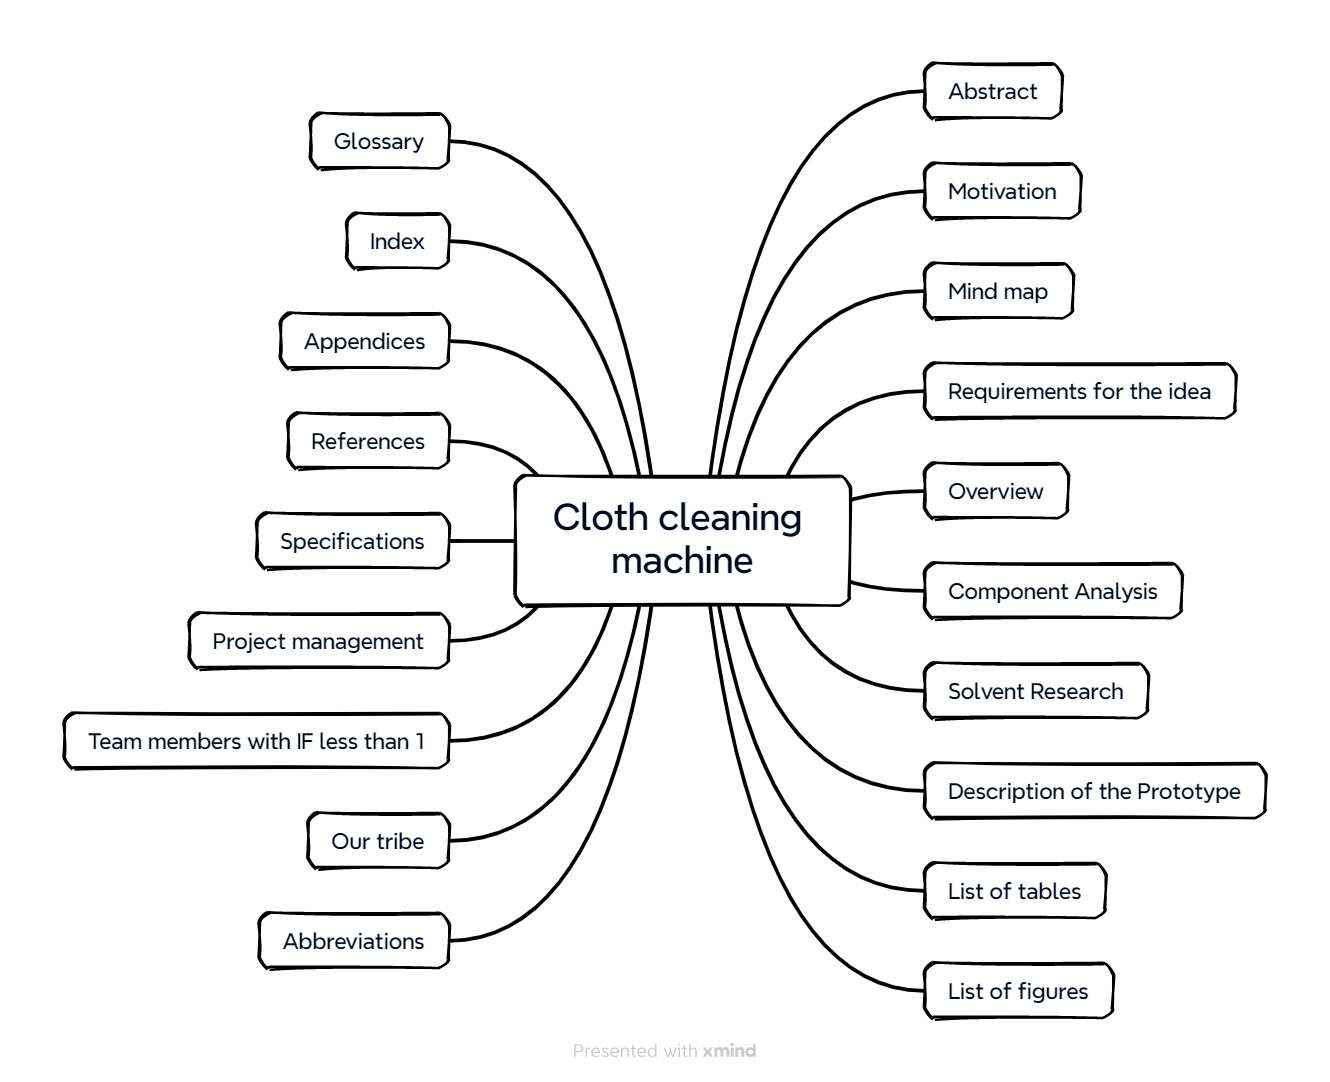
\includegraphics[width=0.9\textwidth]{logos/P1_Outline_TribeD_MindMap_L2.png}
    \caption{Outline Mindmap }
    \label{fig:outlinemindmap}
\end{figure}
\begin{figure}
    \centering
    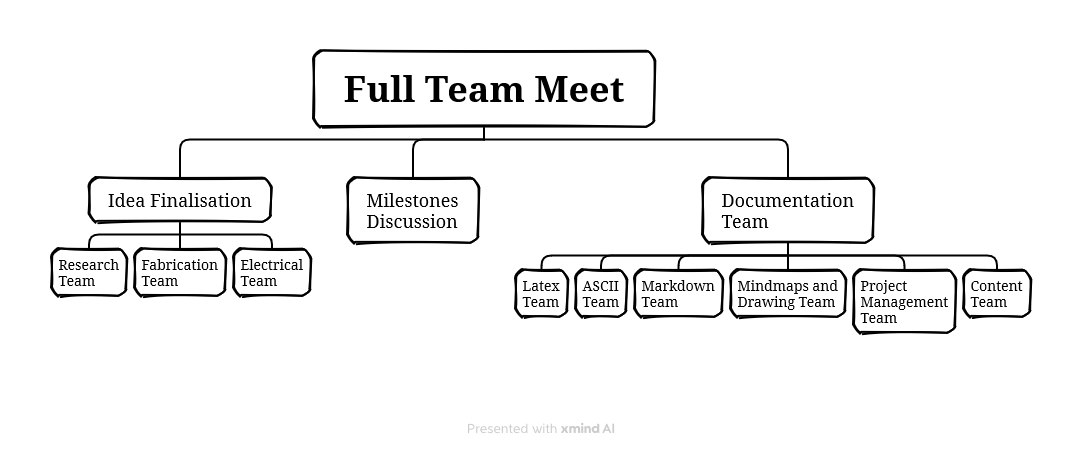
\includegraphics[width=1.1\textwidth]{logos/P1_WorkFlow_TribeD_FlowChart_L3.png}
    \caption{Task Structure}
    \label{fig:outlinemindmap}
\end{figure}
\begin{figure}[htbp]
  \centering
  \begin{adjustbox}{valign=c}
    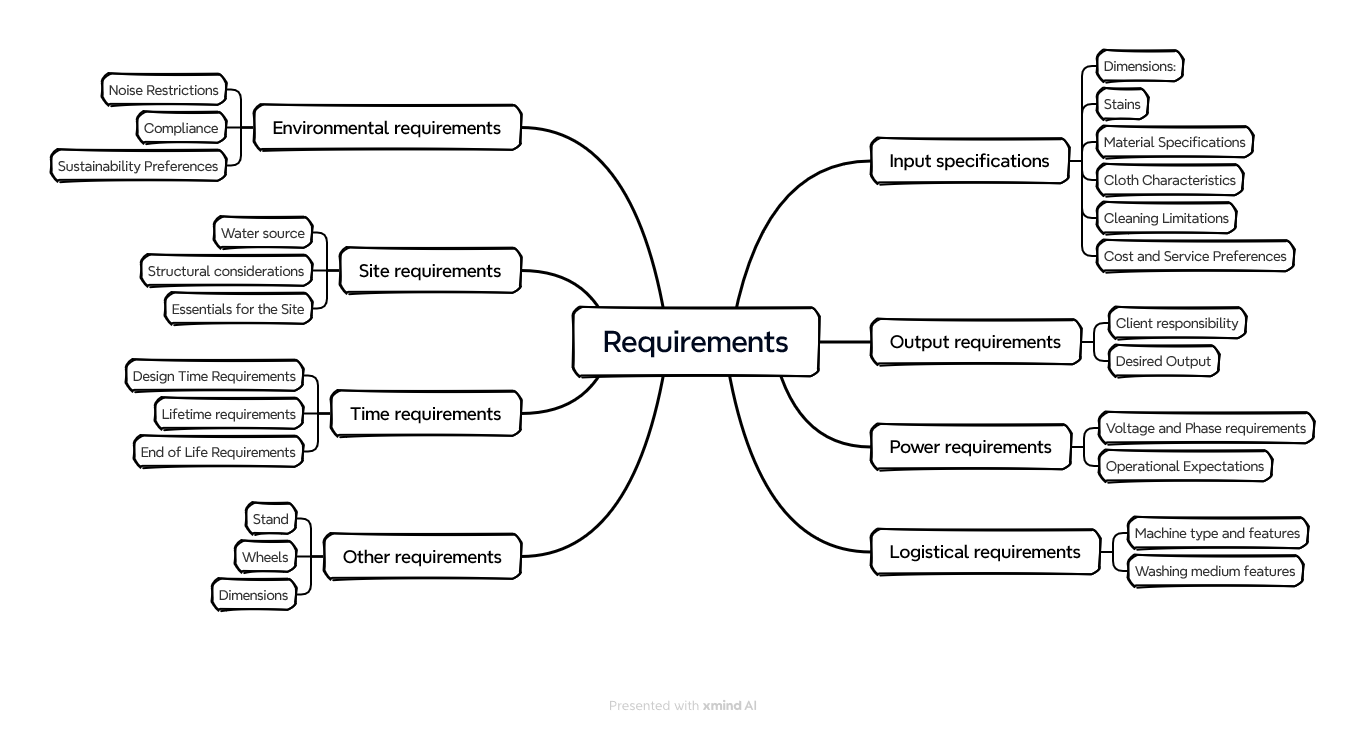
\includegraphics[width=1.1\textwidth]{logos/P1_Req_TribeD_MindMap_L3.png} % Replace 'example-image' with your image file name and extension
  \end{adjustbox}
  \caption{Requirements MindMap}
  \label{fig:reqmindmap}
\end{figure}
\begin{figure}
    \centering
    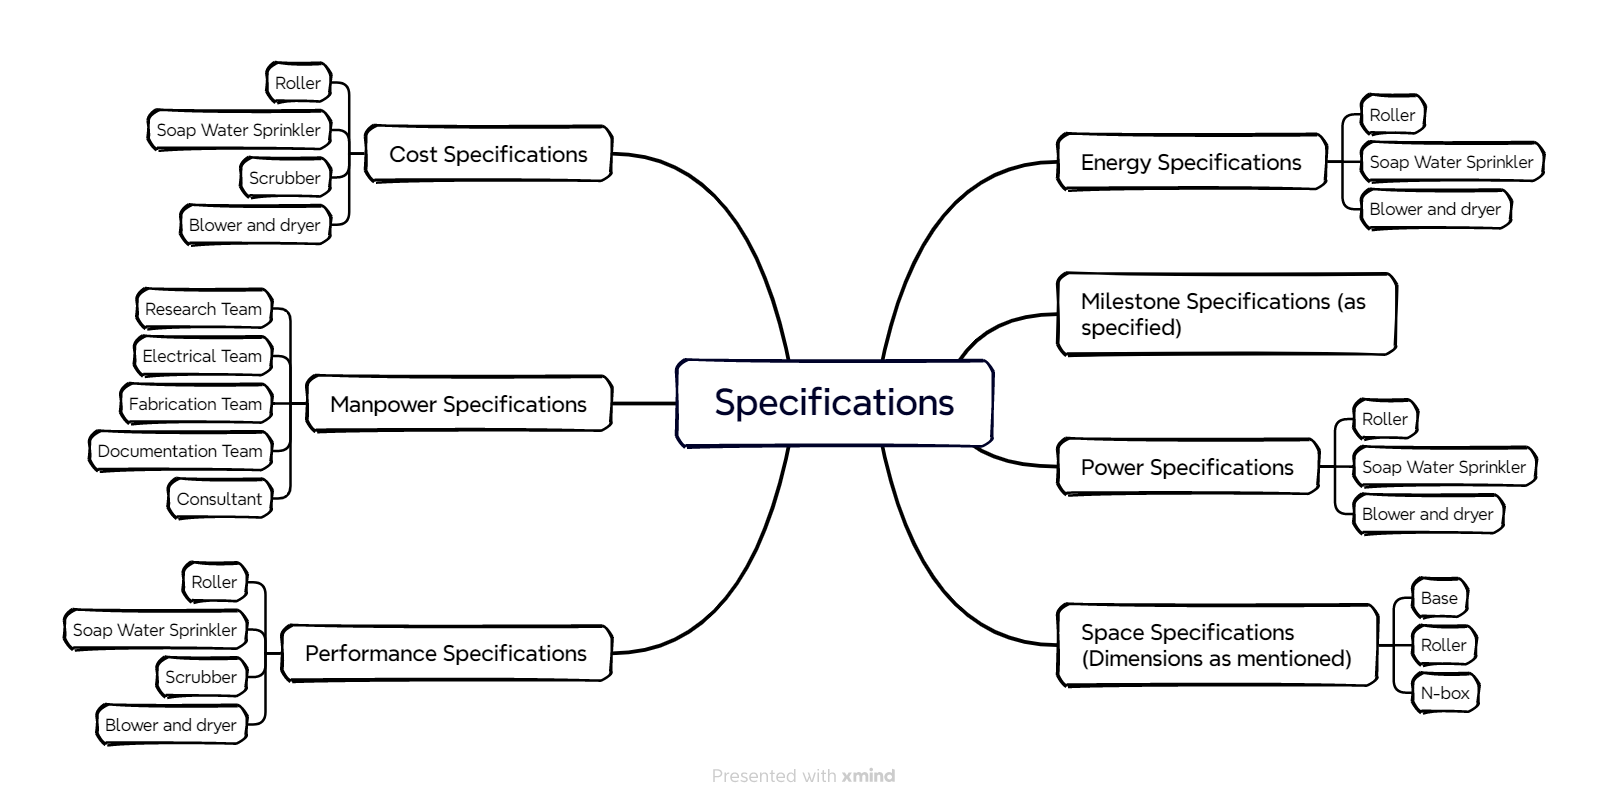
\includegraphics[width=1.1\textwidth]{logos/P1_Specifications_TribeD_MindMap_L3.png}
    \caption{Specifications Mind Map}
    \label{fig:specsmindmap}
\end{figure}

\newpage



\newpage
\pagenumbering{arabic}
\setcounter{page}{1} % Set the starting page number for the main content
\section{Requirements for the idea}\label{sec:requirements}
    

\subsection{ Input Requirements}\label{sec:inputspec}
\subsubsection{Material Requirements}\label{sec:matspec}

    \begin{itemize}[label=$\bullet$]
        \item Newly manufactured white unbleached cotton with single-ply, \index{Denier} \gls{Denier} 60, and a thread count of \gls{threadcount} of 400.
      
    \end{itemize}
\subsubsection{Stains}\label{sec:matspec}
    \begin{itemize}[label=$\bullet$]
      \item Only oil and grease stains present on the edges of the cloth need to be removed.

    \end{itemize}
  
  \subsubsection{Dimensions}\label{sec:dimensions}
    \begin{itemize}[label=$\bullet$]
      \item Cloth is either available on rollers(2m $\times$ 10m) or it can be assumed as an infinite sheet supply of width 2 m.

    \end{itemize}
  
  \subsubsection{Cloth Characteristics}\label{sec:clothchar}
    \begin{itemize}[label=$\bullet$]
      \item Free from foul odour, slightly damp, and without buttons, zippers, or attachments.
    \end{itemize}
  
  \subsubsection{Cleaning Limitations}\label{sec:cleanlim}
    \begin{itemize}[label=$\bullet$]
      \item Maximum weight for cleaning is set at 11 kg dry, with stains\index{stains} limited to those occurring during manufacturing\index{manufacturing}.
    \end{itemize}

% \subsection{ Client Preferences}\label{sec:clientpref}
%     \subsubsection{}{Cost and Service Preferences:}\label{sec:cnspref}
%     \begin{itemize}
%       \item Preference for the washing machine to be offered at zero cost, requiring no servicing time and no maintenance.
%       \item Actual prices are expected to depend on the provider, with alternatives considered if costs are excessively high.
%     \end{itemize}

\subsection{ Outputs Requirement}\label{sec:outputreq}
\subsubsection{Desired Output}\label{sec:desout}
    \begin{itemize}[label=$\bullet$]
      \item A cleaned and dry cloth wound on rollers.
    \end{itemize}
    
% \newpage
\subsubsection{Client Responsibilities}\label{sec:clientresp}
    \begin{itemize}[label=$\bullet$]
      \item Treating discharged \gls{greywater}, \index{greywater} managing lint, and ensuring the returned cloth is wrinkle-free and \gls{bone-dry}. 
    \end{itemize}

\subsection{ Power Requirements}\label{sec:powerreq}
\subsubsection{Voltage and Phase Requirements:}\label{sec: vnpreq}
    \begin{itemize}[label=$\bullet$]
      \item The washing machine should operate on 220VAC 15A, with the option for 440VAC 3-phase available at an additional cost.
    \end{itemize}
  
  \subsubsection{Operational Expectations}\label{sec: opexp}
    \begin{itemize}[label=$\bullet$]
      \item They are expected to run continuously, 24/7, with an emergency shutdown initiated using a 1-button process.
    \end{itemize}

\subsection{Logistical Requirements}\label{sec:logireq}
\subsubsection{Machine Type and Features}\label{sec:machtype}
    \begin{itemize}[label=$\bullet$]
      \item An automatic washing machine with minimal water usage and no need for portability or a programmable timer.
    \end{itemize}
\subsubsection{Washing Medium Features}\label{sec:wmtype}
    \begin{itemize}[label=$\bullet$]
      \item There are no restrictions on the washing medium, but costs may be incurred for using rare solvents, focusing on overall cost-effectiveness.
    \end{itemize}

\subsection{ Environmental Requirements}\label{subsec:envireq}
\subsubsection{Noise and Compliance}\label{sec:noisecomp}
    \begin{itemize}[label=$\bullet$]
      \item Noise levels should not exceed 75 dB.
      \item Must comply with local regulations, including those set by the Central Pollution Control Board (CPCB).
    \end{itemize}
  
  \subsubsection{Sustainability Preferences}\label{sec:suspref}
    \begin{itemize}[label=$\bullet$]
      \item Preference for cold water washing, \index{sustainable} \gls{sustainable} components, and optimization of energy consumption, robustness, and durability.
    \end{itemize}

\subsection{Site Requirements}\label{sec:sitereq}
\subsubsection{Essentials for the Site}\label{sec:essenforsite}
    \begin{itemize}[label=$\bullet$]
      \item Adequate power supply, suitable drainage, and specific design parameters.
    \end{itemize}
  
 \subsubsection{Water Source and Structural Considerations}\label{sec:watersource}
    \begin{itemize}[label=$\bullet$]
      \item The water source was specified as having 60 mg CaCO3/l hardness, with an overhead tank and a 50,000-liter refillable capacity at 35 meters.
      \item Structural considerations include material selection and the ability to withstand the maximum cloth weight.
    \end{itemize}

\subsection{Time Requirements}\label{sec:timereq}
\subsubsection{Cleaning and Setup Time}\label{sec: cnstimes}
    \begin{itemize}[label=$\bullet$]
      \item Cleaning and drying time set at 45 minutes.
      \item Setup time should be at most 1 day.
    \end{itemize}
\subsubsection{Design Time Requirements}\label{sec: destimereq}
    \begin{itemize}[label=$\bullet$]
      \item Cleaning and Drying time: At most  45 minutes.
      \item Usage time: 24 hrs a day.
      \item Setup Time: As little time as possible, no more than 1 day.
    \end{itemize}
  
  \subsubsection{Life-Time Requirements}\label{sec: lifetimereq}
    \begin{itemize}[label=$\bullet$]
      \item Expected Lifetime: The machine is expected to last at least 6 years.
      \item Service Hours and Cost: No more than 6 hours per year and there isn’t an explicit cost constraint for the servicing years.
    \end{itemize}
  \subsubsection{End of Life Requirements}\label{sec: endoflifereq}
    \begin{itemize}[label=$\bullet$]
      \item Replacement for Old Machine: Client could be interested in replacing the old machine for a new one at a discounted price.
      \item Parts Availability:Parts of the machine should be available for 10 years to enable servicing.
    \end{itemize}

\subsection{Other Non-Functional Requirements}\label{sec:otherreq}
\subsubsection{Miscellaneous Considerations}\label{sec:misccons}
    \begin{itemize}[label=$\bullet$]
      \item Dimensions and the inclusion of a stand or wheels are left to the designer's discretion.
      \item We need to clean only edges of the cloth rather the whole cloth.
      \item Only oil stains and grease stains are need to be removed.
      \item Cloth is either available on rollers(2m $\times$ 10m) or it can be assumed as an infinite sheet supply of width 2 m.

    \end{itemize}
\newpage
\section{Overview}
We propose the development of an innovative cloth cleaning machine that can be used to clean oil stains (which occur near the edges) off of manufactured cloth after the manufacturing process. Our design consists of rollers, driving motors, a \gls{guiding frame} \index{guiding frame} (used to fold the cloth in half vertically), wiping and cleaning surface (brushes/sponge), a soap water mixture compartment, a water compartment, and a drying chamber. This automated system aims to streamline the cloth manufacturing process, ensuring efficient cleaning and drying during the manufacturing process while minimising the impact on the fabric. The USP of our design is that the regions of the cloth that are guaranteed to come in clean are untouched in the process, which preserves the quality and durability of the cloth. This approach also ensures that drying requires less effort and resources in comparison to other approaches.
\subsection{Key Components}
\begin{enumerate}[label=\arabic*.]

    \item \textbf{Rollers with Motor Control:}
    \begin{itemize}[label=$\bullet$]
        \item Two rollers placed on either side of the machine.
        \item Motor-controlled to regulate the speed of the cloth movement.
    \end{itemize}

    \item \textbf{Cloth Attachment:}
    \begin{itemize}[label=$\bullet$]
        \item Cloth is securely attached to the rollers upon loading in batches, ensuring uniform tension.
    \end{itemize}

    \item \textbf{Guiding Frame:}
    \begin{itemize}[label=$\bullet$]
        \item Positioned between the rollers upon viewing from the side and placed parallelly between the two vertical walls when viewed from the top.
        \item The frame when viewed from the side looks like a smoothened plateau with a long flat top and curved sides (coming from and going towards the input and output rollers respectively).
        \item Upon viewing from the top, it looks like the edge of a railing.
        \item The frame is slightly angled and is broader at the bottom than at the top.
        \item All edges on the frame are \gls{filleted} \index{filleted} and smoothened to ensure that the cloth doesn’t rip or tear or get stuck while it slides over the frame due to the pull of the motor.
        \item It is shaped this way to guide the fabric to smoothly rise in height from the horizontal roller configuration at the input to the folded vertical configuration in the cleaning and drying chamber.
        \item This vertical folding ensures that the stained edges are hanging on the two sides of the frame symmetrically with the entire cloth folded along the midline and suspended vertically by the normal reaction from the sleek frame.
        \item The part of the fabric towards the centre in the horizontal configuration, now slides at the top of the smooth frame as the rollers on the other end pull it at a constant speed and is unaffected by the cleaning and drying process.
        \item Once the cloth crosses the drying chamber, the guiding frame is shaped in such a way that it lowers the cloth from the raised frame back to its horizontal configuration onto the rollers.
    \end{itemize}

    \item \textbf{Cleaning Mechanism:}
    \begin{itemize}[label=$\bullet$]
        \item Brushes along the edges of the frame at a fixed distance from the height (coincides with the stained edge of the cloth).
        \item The parallel wall also has brushes at the same vertical height, and the two brushes hold on to the edge of the cloth as it moves under the influence of the rollers and scrubs against the brushes, hence getting cleaned.
        \item Solvent drizzled from the top onto the stained part of the cloth). The solvent mixture and water are dispensed in succession and recursively creating stages along the length of the frame. (first “x” cm  $\rightarrow$  soap, next “y” cm $\rightarrow$ water, next “x” cm $\rightarrow$  soap, etc.).
        \item Brushes act as scrubbers to enhance cleaning effectiveness.
    \end{itemize}

    \item \textbf{Cleaning Fluid Compartment:}
    \begin{itemize}[label=$\bullet$]
        \item Alternating compartments for soap water mixture and water.
        \item The soap compartments have brushes along the wall, while the water compartment consists of high-pressure water nozzles to take out the soap from the cloth.
        \item Ensures proper cleaning of the cloth during the process.
    \end{itemize}

    \item \textbf{Drying Chamber :}
    \begin{itemize}[label=$\bullet$]
        \item Located after the cleaning mechanism.
        \item Equipped with \gls{air blowers} \index{air blowers} to blow hot air onto the cloth.
        \item Ensures quick and effective drying.
    \end{itemize}

    \item \textbf{Guiding \gls{Fixtures} : \index{Fixtures}}
    \begin{itemize}[label=$\bullet$]
        \item Transfer the cloth from the input roller to the cleaning chamber of the frame and from the drying chamber of the frame to the rollers.
        \item Facilitates a smooth movement of the cloth.
    \end{itemize}

    \item \textbf{Waste Tub :}
    \begin{itemize}[label=$\bullet$]
        \item A waste tub at the bottom to collect residual drippings and lint.
    \end{itemize}

\end{enumerate}
% \begin{figure}[h]
%     \centering
%     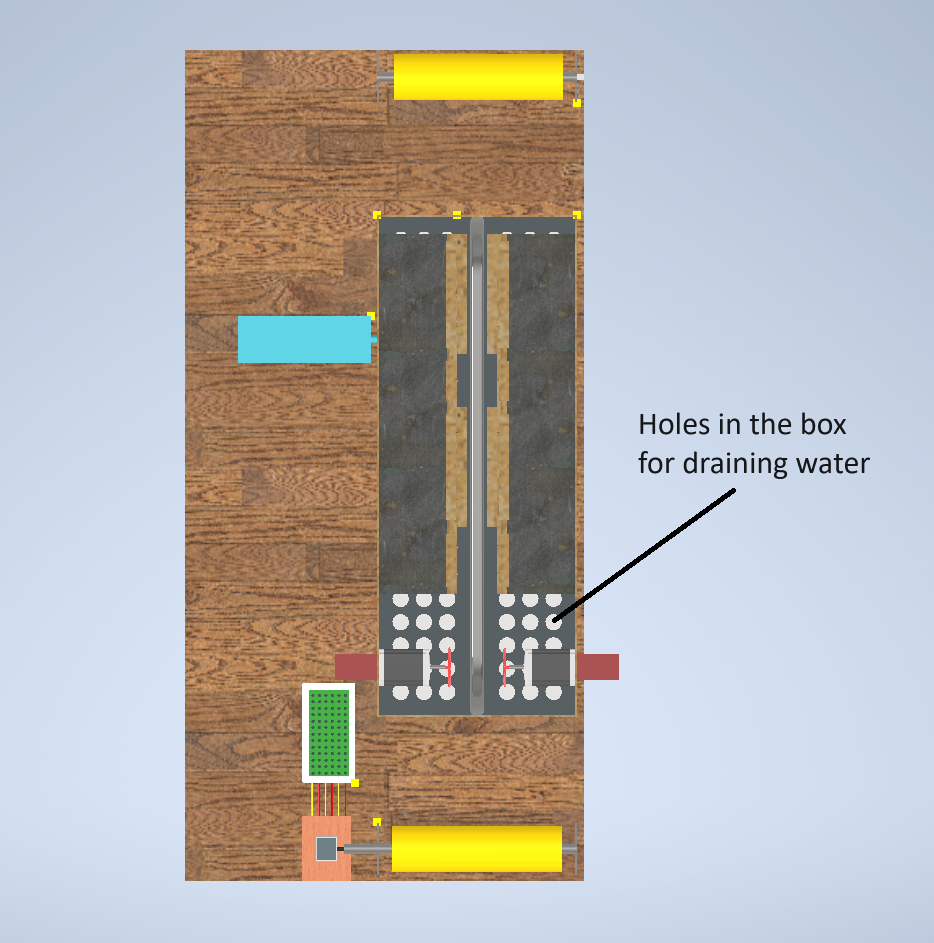
\includegraphics[width=0.6\textwidth]{logos/top_view.png}
%     \caption{Top view of the final CAD model }
%     \label{fig:topview}
% \end{figure}
\begin{figure}[h]
    \centering
    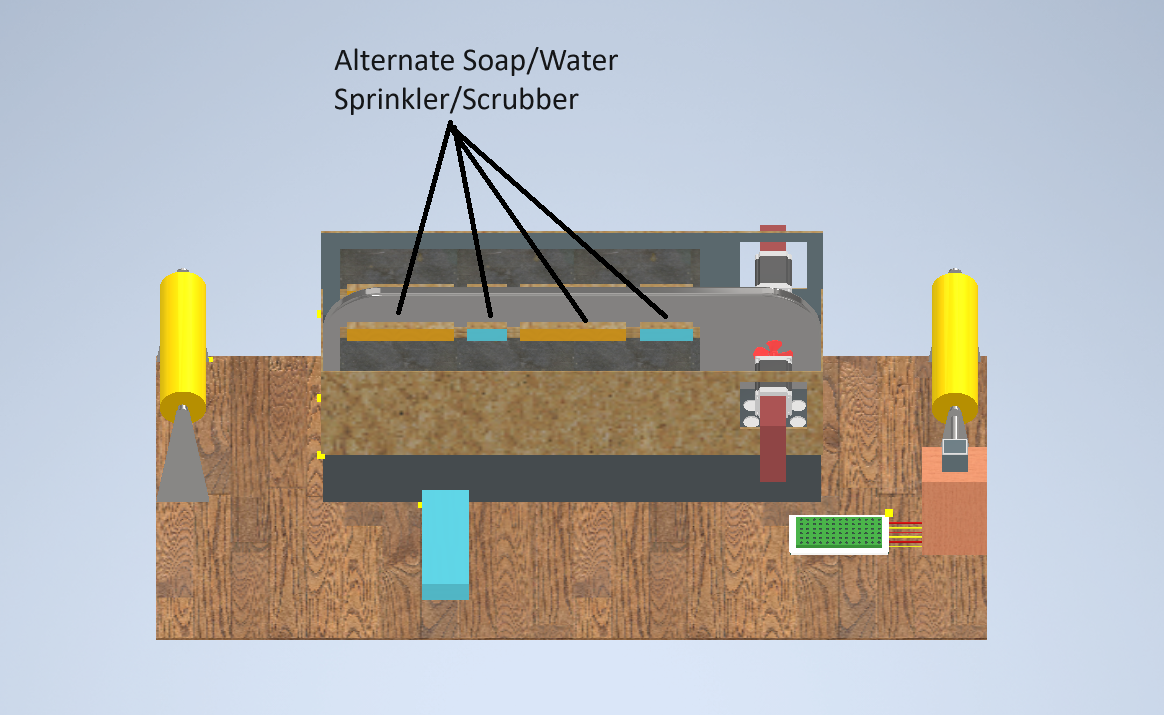
\includegraphics[width=0.70\textwidth]{logos/side_view.png}
    \caption{Side view of the final CAD model}
    \label{fig:sideview}
\end{figure}
\begin{figure}[h]
    \centering
    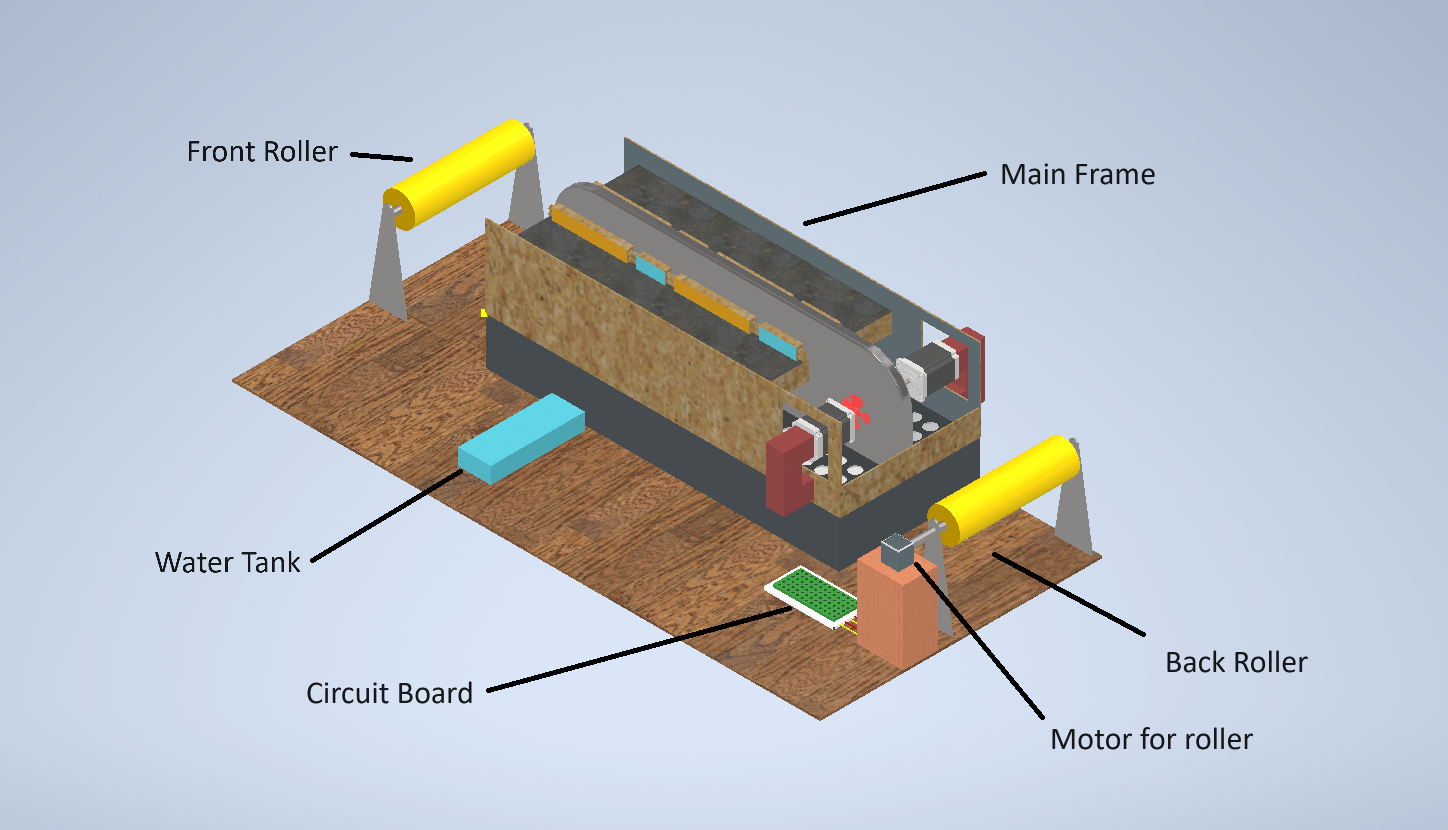
\includegraphics[width=0.70\textwidth]{logos/iso_view.png}
    \caption{Isometric view of the final CAD model}
    \label{fig:isometricview}
\end{figure}
\newpage
\subsection{WorkFlow}
\begin{enumerate}[label=$\bullet$]

    \item Cloth is loaded onto input rollers over the guiding frame, through the cleaning and drying chamber and onto the output roller. In order to prevent wastage of a significant initial length of the cloth roll, we can attach it to a clean dummy cloth of machine length, with the help of a speed punching system and later detach the dummy cloth and reuse it for the next batch. This is not relevant for demonstration but crucial during industrial scaling.

    \item Then a lever/switch is activated which brings the two walls closer to the guiding frame with the cloth attached to it and the horizontal line of brushes lock onto each hanging edge of the cloth securing it in place.

    \item Motors are powered on, and the cloth starts sliding on the frame while being kept in place by the walls and guiding fixtures.

    \item The Solvent is drizzled from the top with targeted precision on the edges, and brushes act as scrubbers for thorough cleaning as the cloth slides over them.

    \item The cloth passes through multiple alternating soap water mixture and water compartments and gets recursively cleaned for better results.

    \item The cloth then enters the drying chamber, where hot air is blown to expedite the drying process.

    \item After drying, the cleaned and dried cloth moves through guiding fixtures onto the rollers for subsequent manufacturing processes.

\end{enumerate}
\subsection{Benefits}
\begin{enumerate}[label=$\bullet$]
    \item Improved cloth cleaning efficiency.
    \item Minimized impact on the fabric during the cleaning process.
    \item Streamlined manufacturing workflow.
    \item Enhanced drying capabilities for increased production speed.
\end{enumerate}
\textbf{Calculation of order of magnitude of the length of chamber:}
\begin{itemize}[label=$\bullet$]
    \item Load in one batch = 11 kg.
    \item Breadth of cloth roll = 2 m.
    \item The \gls{Areal density} \index{Areal density} of Single ply cotton cloth unbleached, denier 60, thread count 400 = 0.180 kg/m\textsuperscript{2}.
    \item Time provided for cleaning = 45 minutes.
    \item \( l = \frac{90 \times 11}{0.18 \times 2 \times 45 \times 60} \) m =1 m approx = 40 inches approx (l = cleaning and drying length).
    \item Varying soaps changes the time cloth needs to spend in the chamber which increases/decreases the length of the machine.

\end{itemize}
% \newpage


\section{Component Analysis}\label{sec:compana}
\subsection{Roller}\label{sec:roller}
\begin{enumerate}
  \item The roller will roll the washed cloth, coming through the conveyor belt.
  \item A controlled DC motor\index{motor} will be used to drive the roller.
  \item Appropriately select the dimensions of the roller, like the diameter of the roller and its length, based on the conveyor width.
  \item Choose a proper outer covering for the roller, which can provide a better grip and friction for the cloth.
  \item The cloth will also be straightened using 1 or 2 uncontrolled rolling cylinders which can provide the requisite tension in the fabric and guide the fabric onto the roller.
\end{enumerate}
% \vspace{1.5cm}
\begin{figure}[h]
    \centering
    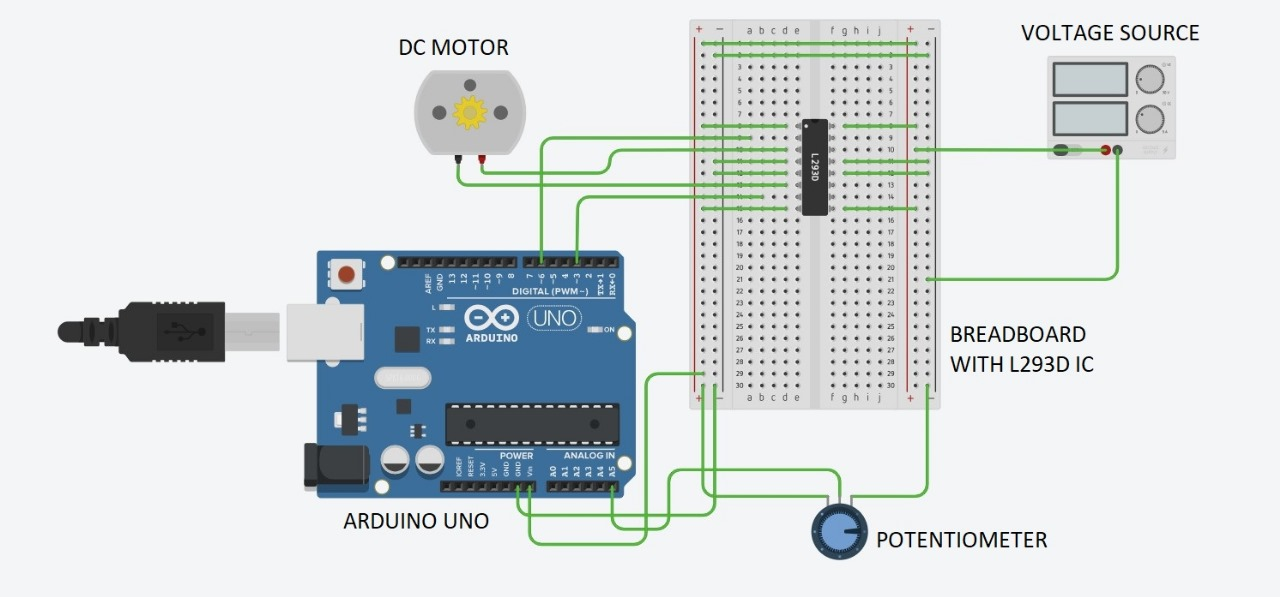
\includegraphics[width=0.6\textwidth]{logos/roller_circuit.jpeg}
    \caption{Circuit diagram for controlling roller's motor }                   
    \label{fig:outlinemindmap}
\end{figure}
% \newpage

\subsubsection{Controlling DC Motor using Arduino\index{Arduino}}\label{sec:contdcmotor}

To control the speed of a DC motor\index{motor} using \gls{Arduino}\index{Arduino}, we need to adjust the input voltage\index{voltage} supplied to the motor\index{motor}. 
We can control the input voltage\index{voltage} with a pulse-width modulated (PWM) signal.
To change the speed of the DC motor\index{motor} we need to change the amplitude of the input voltage\index{voltage} that is applied to the motor\index{motor}.
A common technique to do that is PWM (Pulse Width Modulation). In PWM the applied voltage\index{voltage} is adjusted by sending a series of pulses so the output voltage is proportional pulse width generated by the \index{microcontroller} \gls{microcontroller} that is also known as duty cycle.
\newpage
\begin{figure}[h]
    \centering
    
\includegraphics[width=1.1\textwidth]{logos/roller_wavedrom_new.png}
    \caption{A square wave with 50\% duty cycle}
    \label{fig:outlinemindmap}
\end{figure}
The higher the duty cycle, the higher the average voltage applied to the DC motor\index{motor} (resulting in higher speed) and the shorter the duty cycle, the lower the average voltage applied to the DC motor\index{motor} (resulting in lower speed).

\subsubsection{Arduino and L293D Circuit Diagram}\label{sec:adriono}
A common and cheap solution to drive motor\index{motor}s and efficiently control them is to use a Motor \gls{Controller} \index{Controller} module along with Arduino. L293D Motor driver module is a readily available IC which can be easily interfaced with Arduino, to control the various aspects of DC motors\index{motors} like speed, direction and braking. It is designed to provide bidirectional\index{bidirectional} drive currents of up to 600-mA at voltages from 4.5 V to 36V.
Below is an example of a circuit diagram to drive multiple motors\index{motors} from a single module, and Arduino\index{Arduino} code to interface a motor with the module.

% \item \href{}\textcolor{blue}{Click here for arduino code}}

\begin{lstlisting}
# Define constants for pin numbers
leftForward = 6
leftBackward = 3
pot = A5

# Initializing some variables
pwm
x

# Running the Setup function once at the beginning
setup() 

  # Set the leftForward and leftBackward as outputs and pot as an input
  pinMode(leftForward , OUTPUT)
  pinMode(leftBackward , OUTPUT)
  pinMode(pot, INPUT)

  # Begin serial communication for debugging
  Serial.begin(9600)

# Loop function to run repeatedly
loop()
  # Reading the analog value from pot
  pwm = analogRead(pot)
  # mapping the value of pwm within appropriate bounds
  x = map(pwm, 0, 1023, 0, 255);
  # Assigning the value of pwm to x, and configuring the values to drive the motor in a particular direction 
  analogWrite(leftForward , x);
  digitalWrite(leftBackward , LOW);
\end{lstlisting}
\item \href{https://github.com/naunidhsingh03/ELP305-TribeD-Resources/blob/5ba1988fe283faba21ba7098978bb225e509d5cb/Codes/final_roller.ino}
{\textcolor{blue}{Click here for the Arduino code reference}}

% \newpage
\subsection{Soap Water Requirements}
\subsubsection{A. For split cloth pieces using sensor}

\begin{lstlisting}
const int poten = A3;
int var;

void setup()
{
  pinMode(6, OUTPUT);
}

void loop()
{
  var = analogRead(poten);
  analogWrite(6, var);
}

\end{lstlisting}
\vspace{0.5cm}
\begin{figure}[h]
    \centering
    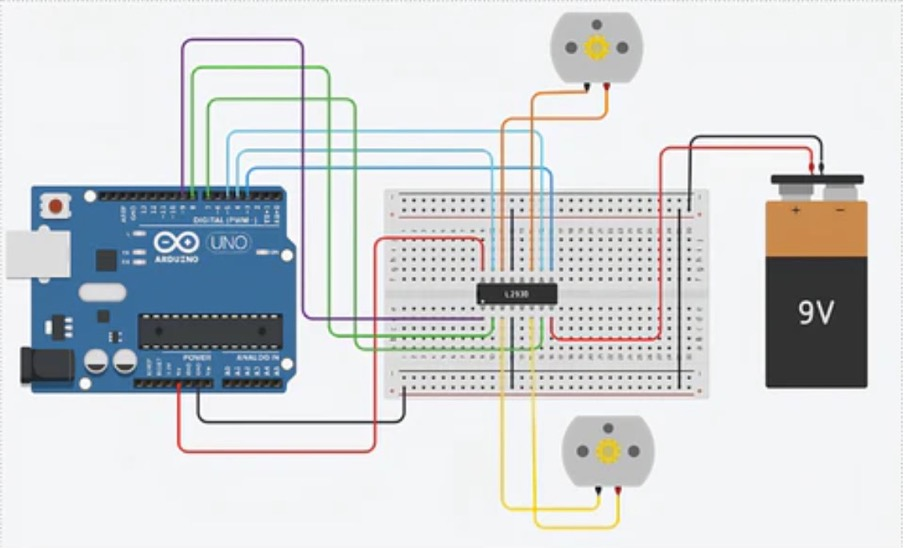
\includegraphics[width=0.5\textwidth]{logos/adriono.jpg}
    \caption{Sample circuit diagram of motor control}
    \label{fig:outlinemindmap}
\end{figure}
\newpage
\begin{figure}[h]
    \centering
    \vspace{2cm}
    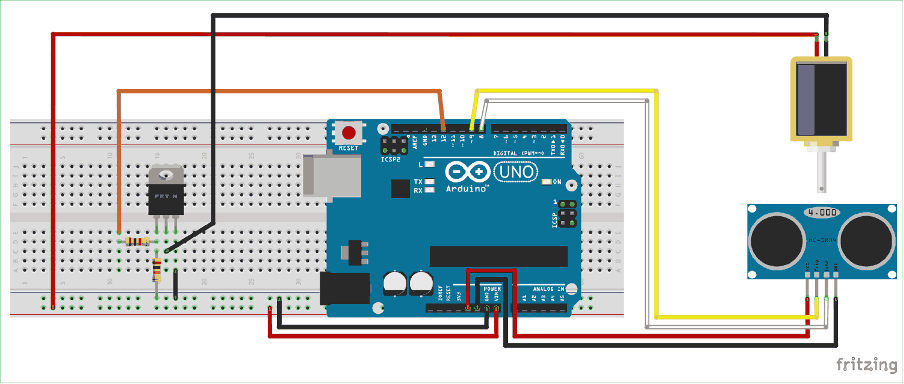
\includegraphics[width=0.87\textwidth]{logos/soap1.png}
    \caption{  For cut cloth pieces using sensor}
    \label{fig:outlinemindmap}
\end{figure}

%\href{https://github.com/naunidhsingh03/ELP305-TribeD-%Resources/blob/5ba1988fe283faba21ba7098978bb225e509d5cb/Codes/solvent_dispense%r_old_design_1.ino}{\textcolor{blue}{Click here for the code reference}}
\subsubsection*{Explanation:}
\begin{itemize}[label=$\bullet$]
    
\item When the distance is less than 10cm, we have to turn on the MOSFET, and otherwise, we have to turn off the MOSFET. We will also use the on-board LED connected to pin 13 and toggle it along with the MOSFET so that we can ensure if the MOSFET is in the turned-on or turned-off state.

\item Inside the main loop function, we call for the function called \texttt{measure\_distance()}. This function uses the US sensor to measure the distance of the object in front of it and updates the value to the variable \texttt{distance}.

\item The input or the detection will send a sonic blast of Ultrasonic signals into the air, which will get reflected by the object in front of it, and the echo pin will pick up the signals reflected by it. Then we use the time taken value to calculate the distance of the object ahead of the sensor.

\item Once the distance is calculated, we have to compare the value of distance using a simple if statement. If the value is less than 10cm, we make the MOSFET and LED go high. In the following else statement, we make the MOSFET and LED go low.
\end{itemize}

\newpage
\subsubsection{B. Without Sensor, using push button}
\begin{figure}[h]
    \centering
    \begin{subfigure}{0.4\textwidth}\label{sec:figone}
        \centering
        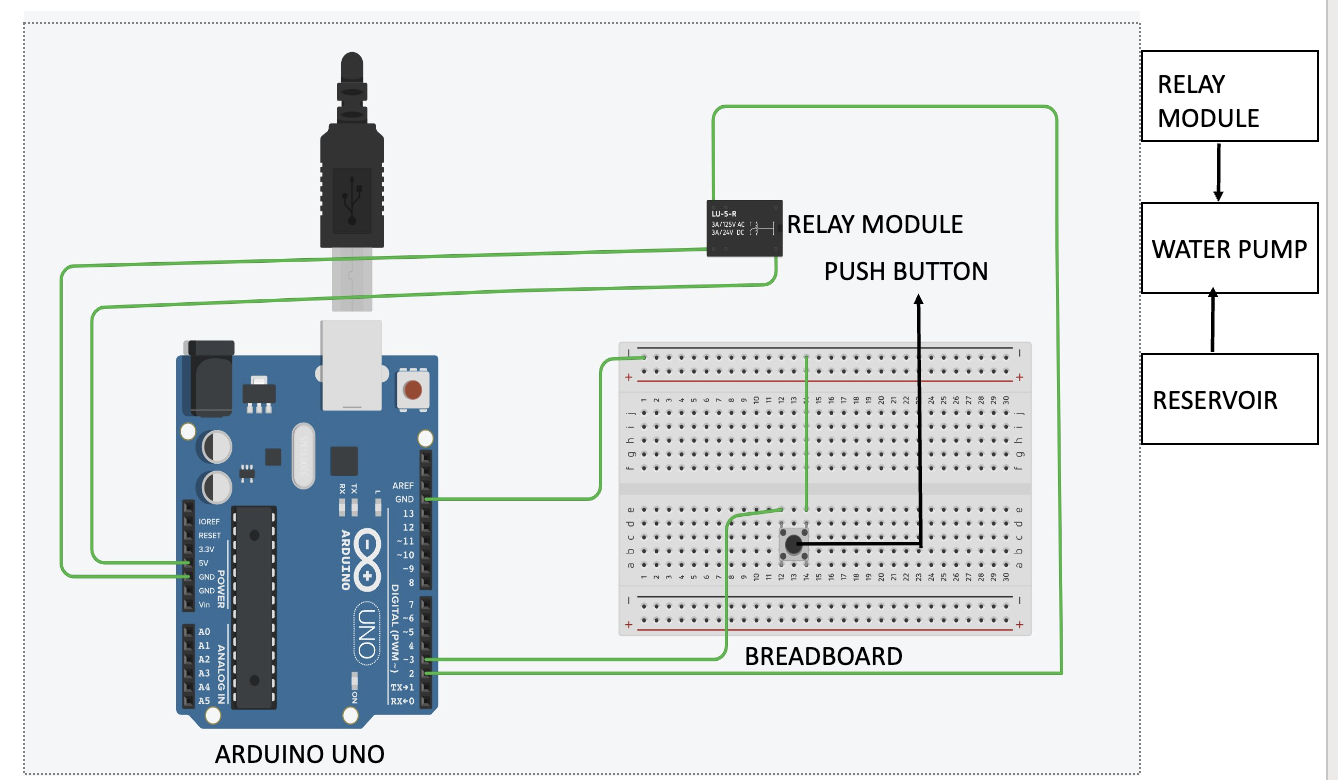
\includegraphics[width=\linewidth]{logos/push_button.png}
        \caption{Using Push Button}
    \end{subfigure}\hspace{0.1\textwidth}%
    \\
    \vspace{0.5cm}
    \begin{subfigure}{0.5\textwidth}\label{sec:figtwo}
        \centering
        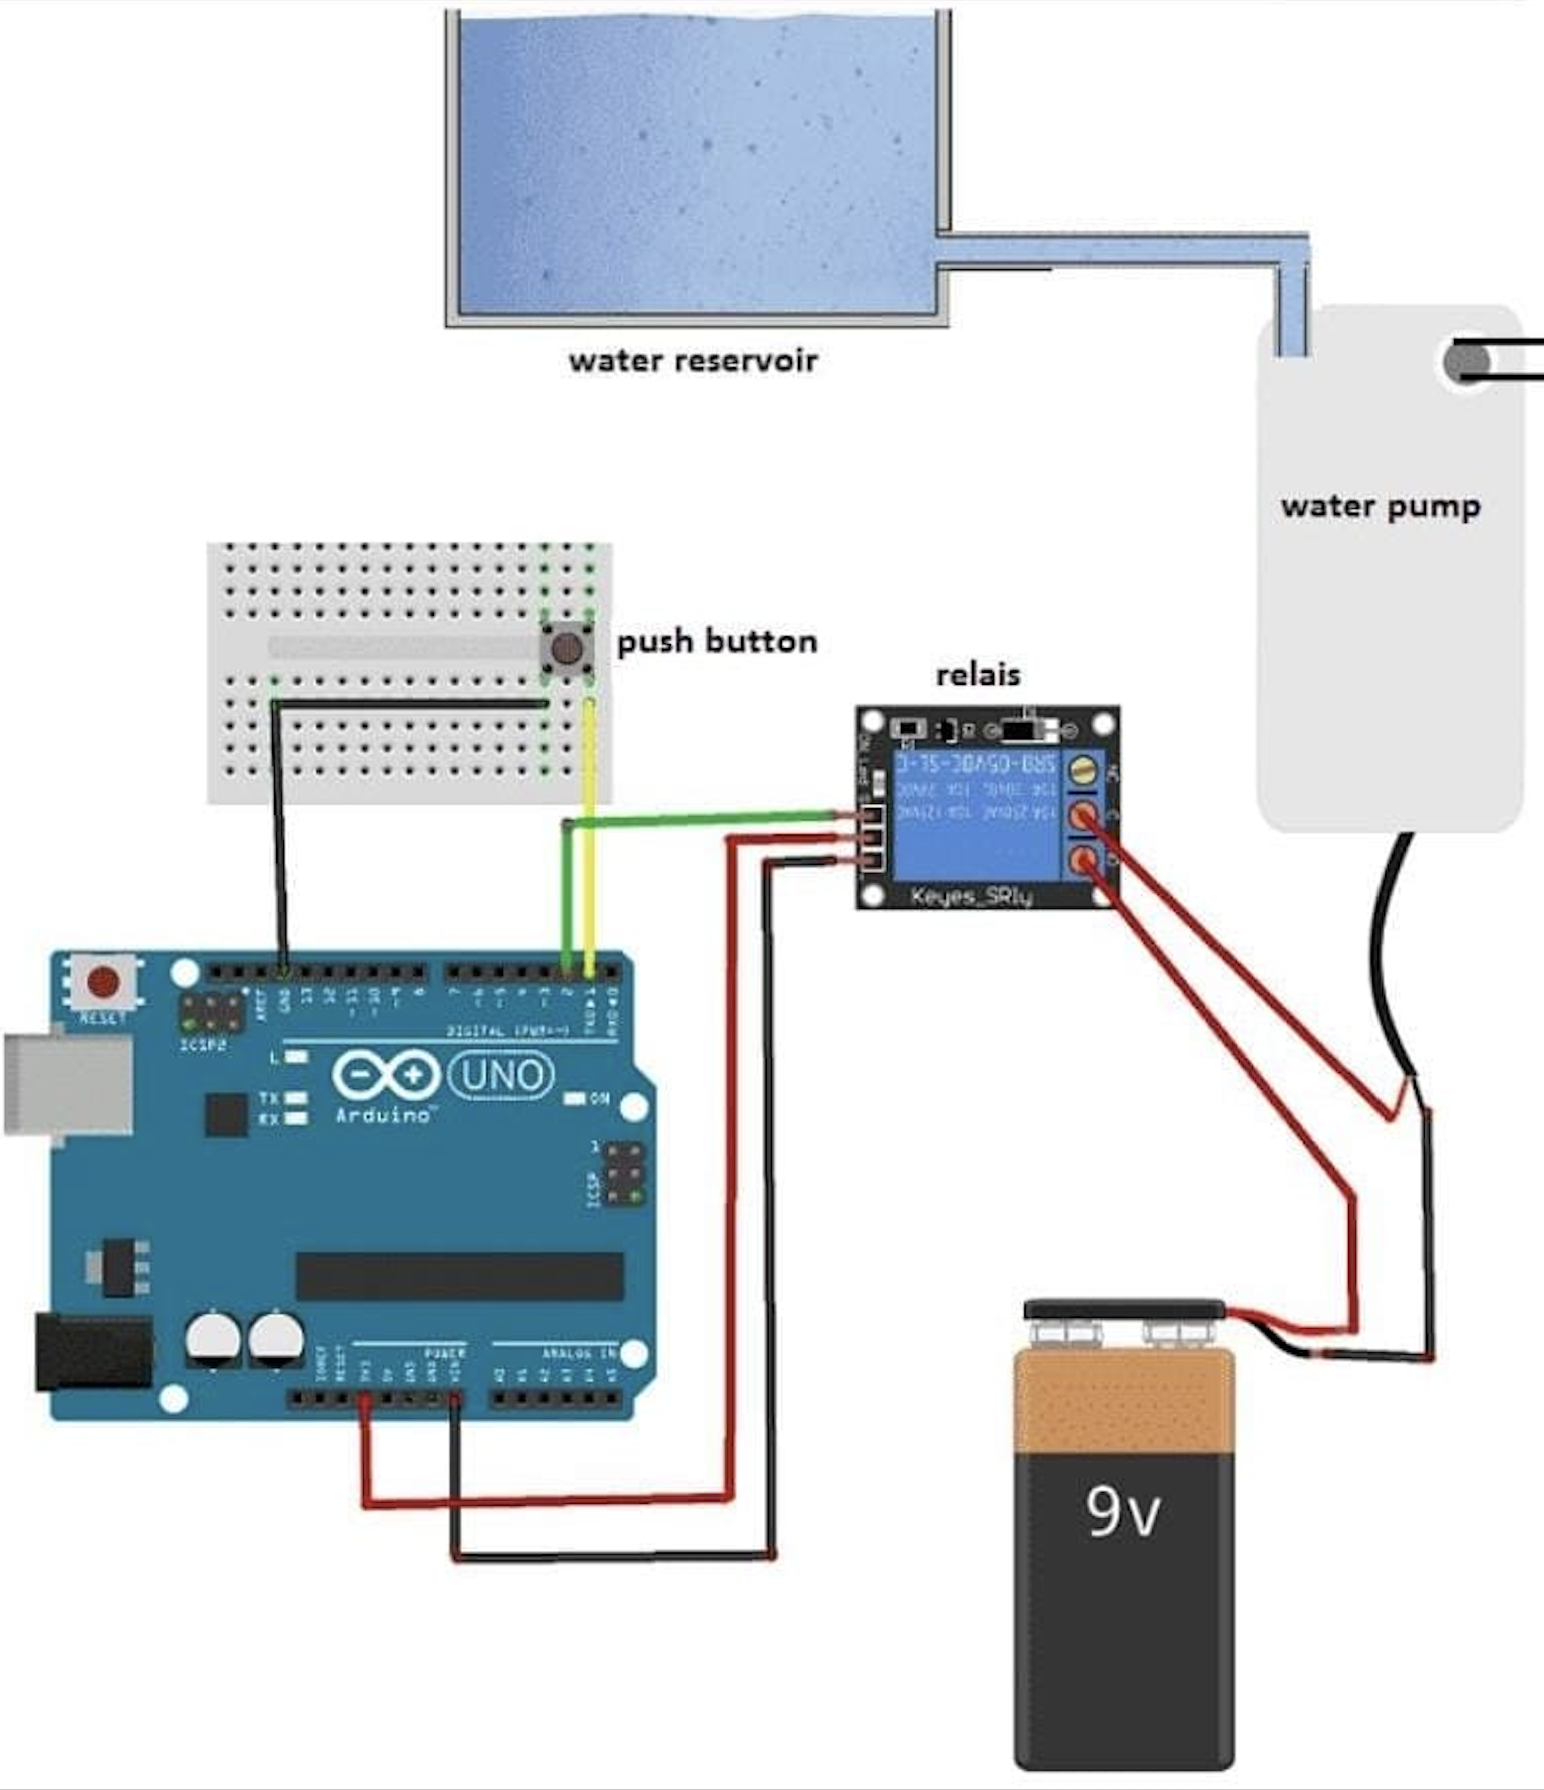
\includegraphics[width=\linewidth]{logos/sprinkler.png}
        \caption{Full circuit}
    \end{subfigure}
    \caption{Sprinkler}
\end{figure}
% \newpage

\subsubsection*{Explanation}
\begin{itemize}[label=$\bullet$]
    \item A push button is employed to toggle the relay, managing the on/off state of the pump.
    \item The relay is cycled at regular intervals, simulating control over a device, such as a solvent pump.
     To activate the relay, the relay pin (control pin) is set to HIGH.
     To deactivate the relay, the relay pin is set to LOW.
\end{itemize}
\newpage

\href{https://github.com/naunidhsingh03/ELP305-TribeD-Resources/blob/5ba1988fe283faba21ba7098978bb225e509d5cb/Codes/solvent_spinkler_new_design_1.ino}{\textcolor{blue}{Click here for code reference}}
% \begin{figure}[h]
%     \centering
%     \begin{subfigure}{0.4\textwidth}\label{sec:figone}
%         \centering
%         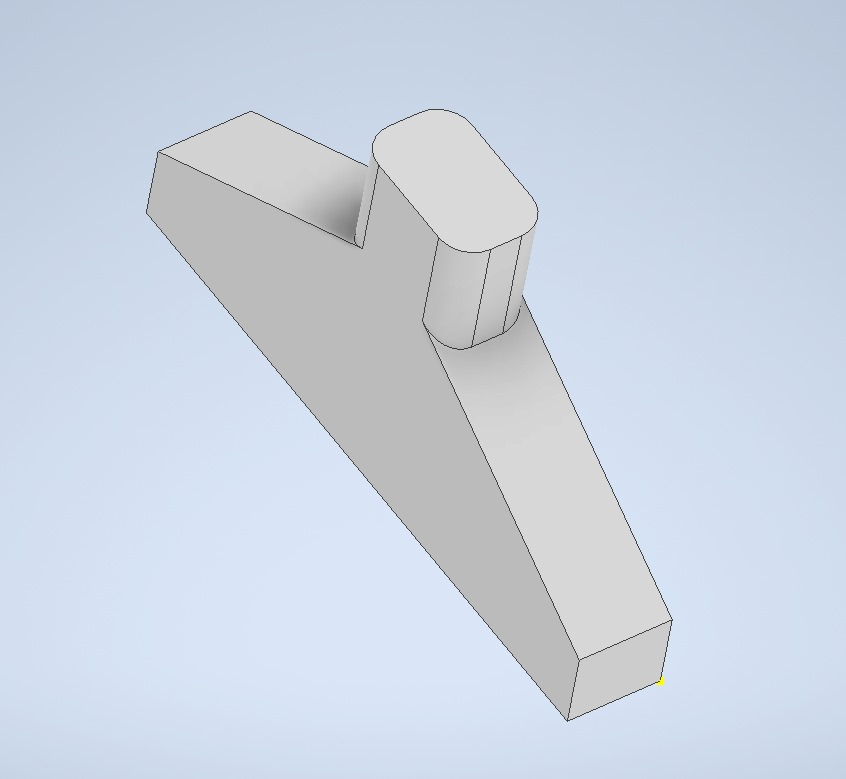
\includegraphics[width=\linewidth]{logos/sprinkler fig1.png}
%         \caption{Isometric View\index{\gls{Isometric View}1}}
%     \end{subfigure}\hspace{0.1\textwidth}%
%     \begin{subfigure}{0.5\textwidth}\label{sec:figtwo}
%         \centering
%         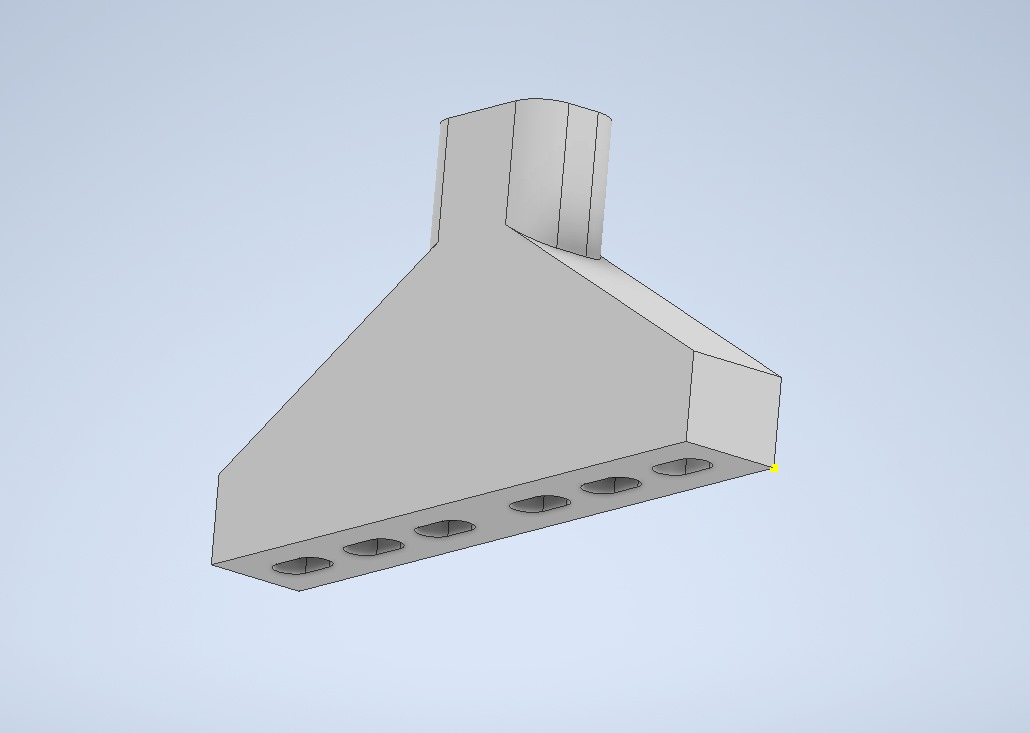
\includegraphics[width=\linewidth]{logos/sprinkler fig2.png}
%         \caption{Isometric View\index{\gls{Isometric View}}2}
%     \end{subfigure}
%     \caption{Sprinkler}
% \end{figure}
% \newpage
% \subsection{Solvent Sprinkler}
% \begin{figure}[h]
%     \centering
%     \begin{subfigure}{0.4\textwidth}\label{sec:figone}
%         \centering
%         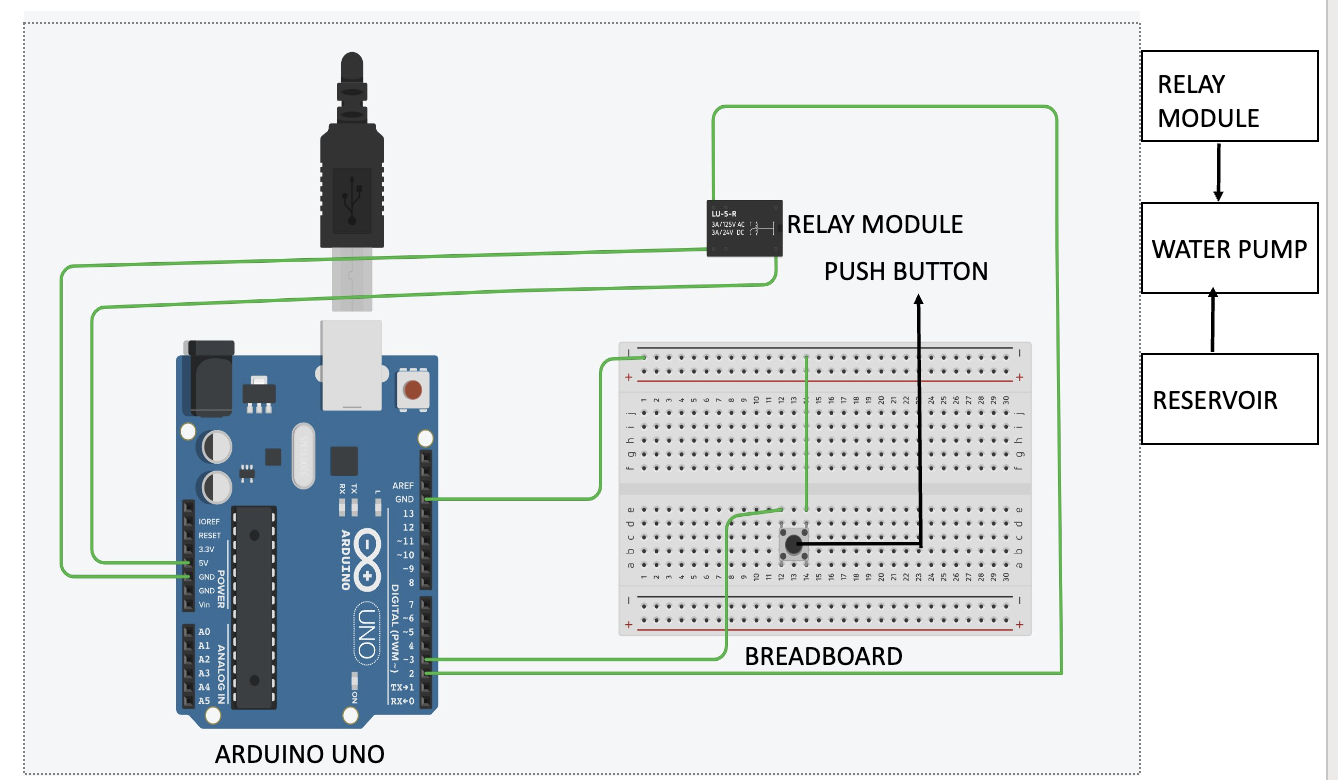
\includegraphics[width=\linewidth]{logos/push_button.png}
%         \caption{Using Push Button}
%     \end{subfigure}\hspace{0.1\textwidth}%
%     \begin{subfigure}{0.5\textwidth}\label{sec:figtwo}
%         \centering
%         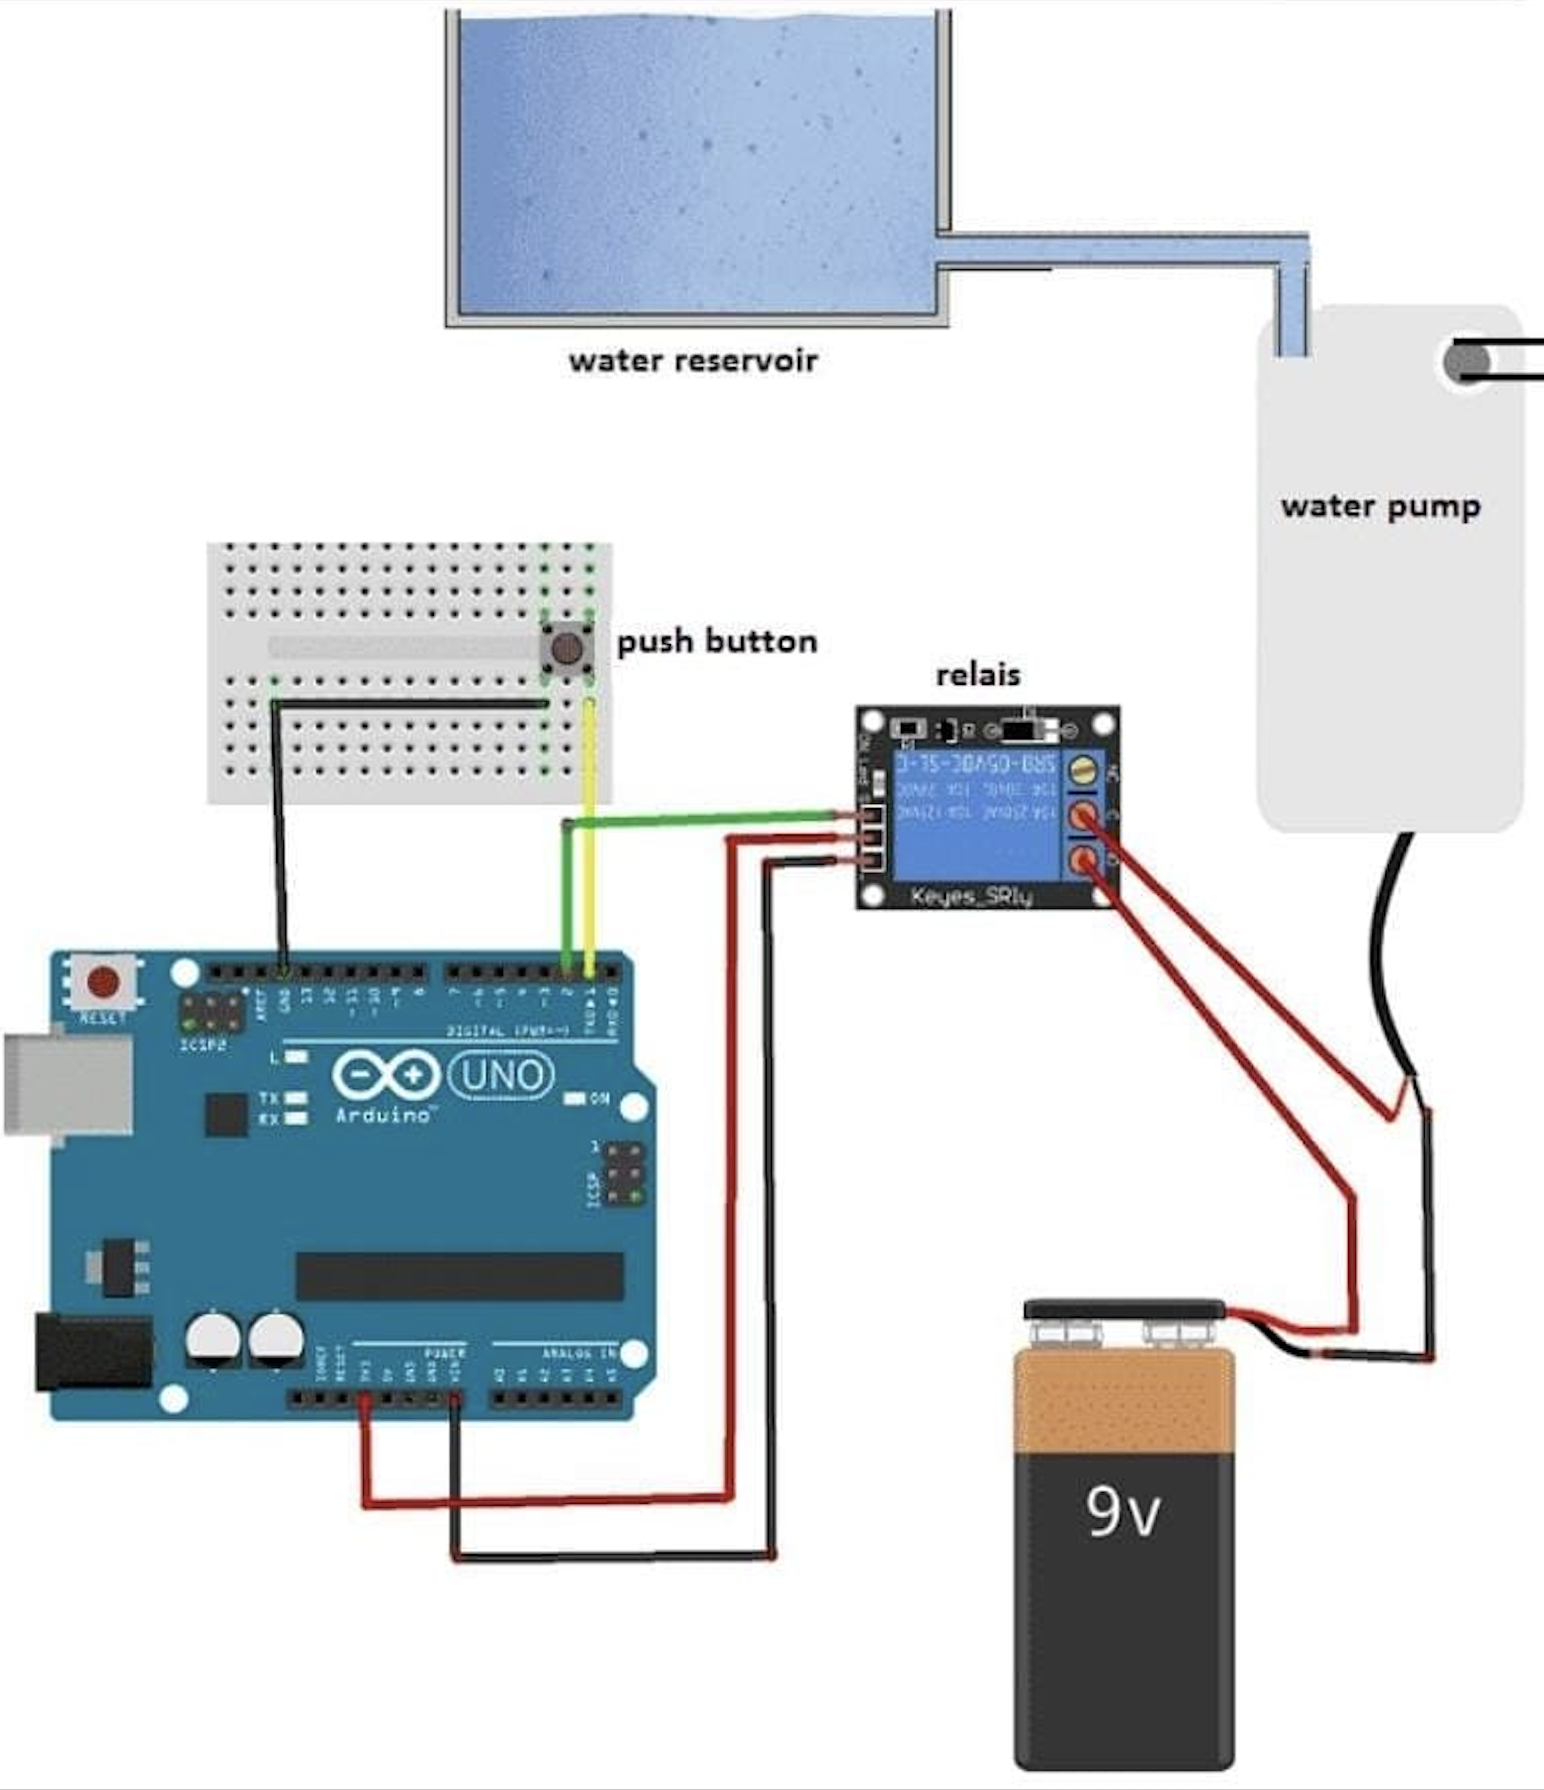
\includegraphics[width=\linewidth]{logos/sprinkler.png}
%         \caption{Full circuit}
%     \end{subfigure}
%     \caption{Sprinkler}
% \end{figure}
\begin{lstlisting}
# Define constants for pin numbers
relayPin = 2
buttonPin = 3

# Setup function to run once at the beginning
setup():
    # Set the relayPin as an output and buttonPin as an input with pull-up resistor
    pinMode(relayPin, OUTPUT)
    pinMode(buttonPin, INPUT_PULLUP)
    
    # Begin serial communication for debugging
    Serial.begin(9600)
    
    # Turn off the relay initially
    digitalWrite(relayPin, LOW)

# Loop function to run repeatedly
loop():
    # Read the state of the button (HIGH or LOW)
    buttonState = digitalRead(buttonPin)
    
    # Print the button state for debugging
    Serial.println(buttonState)
    
    # Check if the button is pressed (LOW state)
    if buttonState is LOW:
        # Turn on the relay
        digitalWrite(relayPin, HIGH)
    else:
        # Turn off the relay
        digitalWrite(relayPin, LOW)
\end{lstlisting}

% \begin{figure}[h]
%     \centering
%     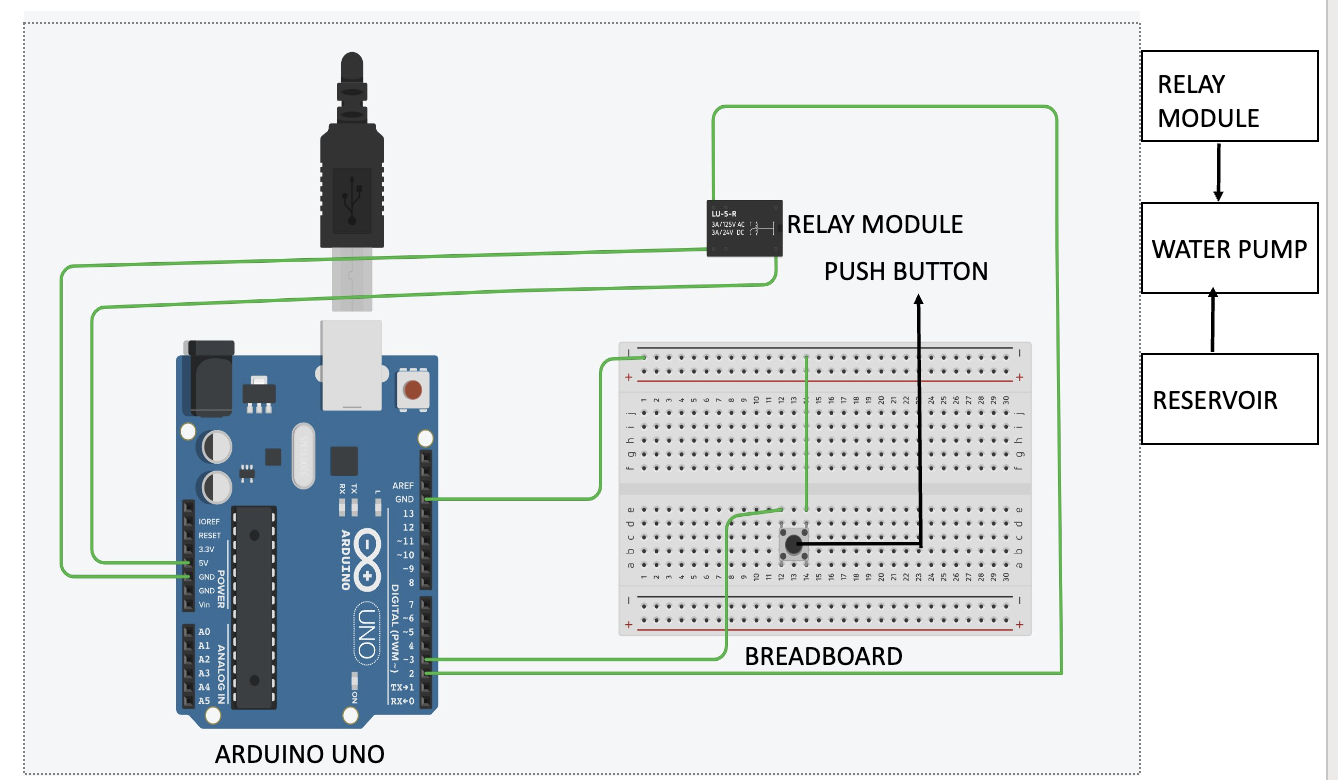
\includegraphics[width=0.4\textwidth]{logos/push_button.png}
%     \caption{Push Button}
%     \label{fig:outlinemindmap}
% \end{figure}
% \begin{figure}[h]
%     \centering
%     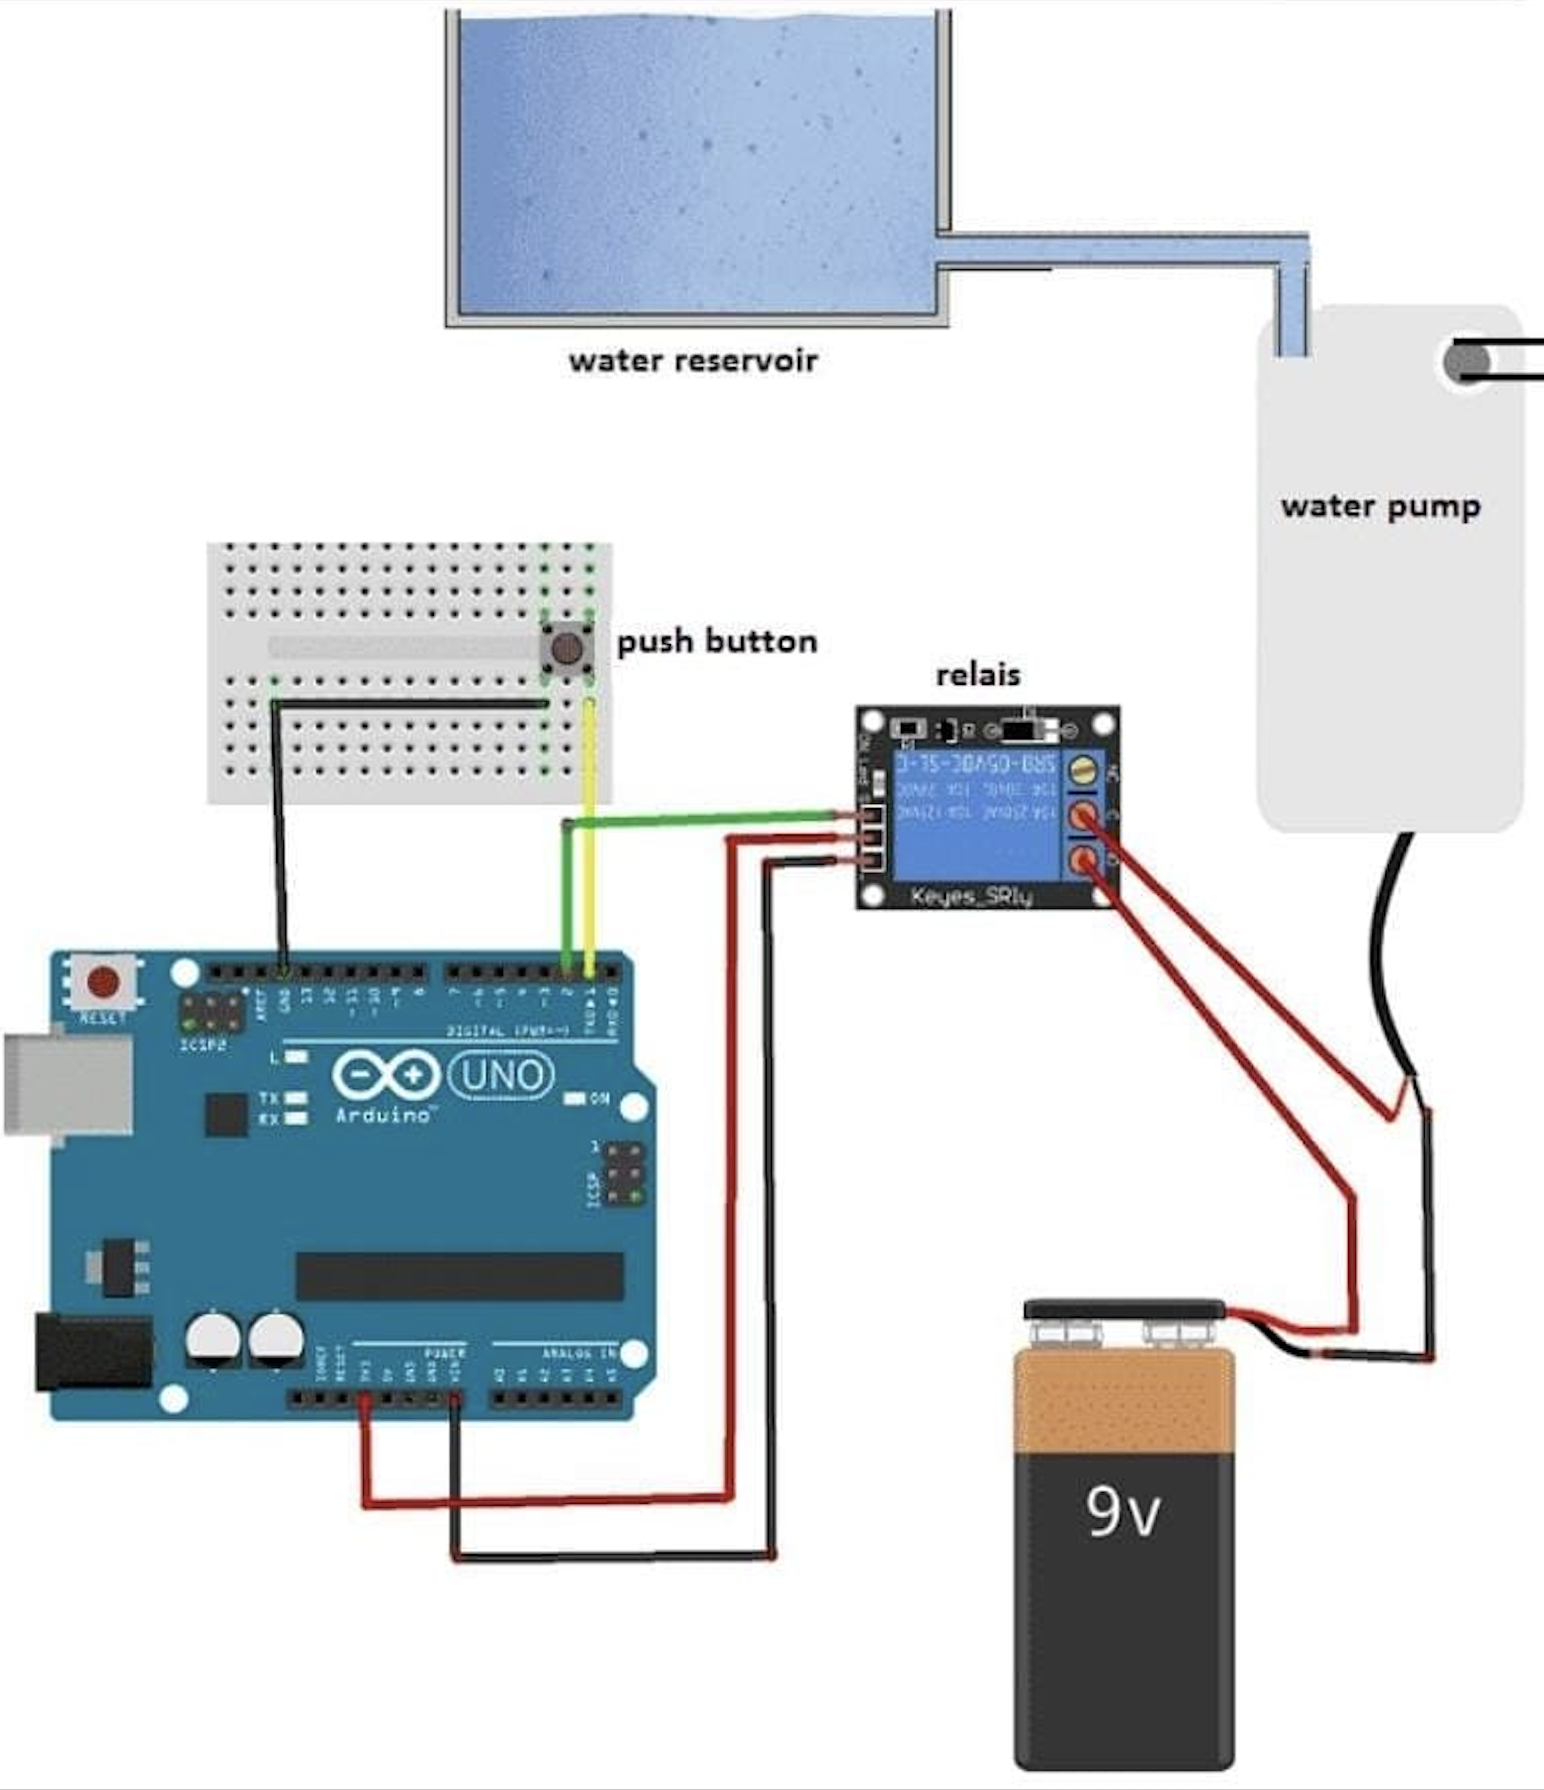
\includegraphics[width=0.5\textwidth]{logos/sprinkler.png}
%     \caption{Sprinkler}
%     \label{fig:outlinemindmap}
% \end{figure}

% \newpage

\subsection{Scrubber}
\begin{itemize}[label=$\bullet$]
    \item Static stationary brush scrubber is an industrial cleaning tool designed for efficient cloth cleaning. This device features stationary brushes that remain fixed during operation, providing a stable cleaning surface. The static design allows for controlled and targeted cleaning of fabrics, ensuring uniform and effective removal of dirt and contaminants. This type of scrubber is commonly employed in industrial settings where precision and consistency in cloth cleaning are essential for maintaining high standards of hygiene and product quality.
    \item Stationary brushes would be used near the edges of the cloth.
    \item Static cleaning mechanism.
    % \item Zero power requirement
    % \item Specifications:
    
\end{itemize}

\subsection{Dryer}
We are planning to use the configuration of tunnel dryer to dry the clothes. The power and torque requirements of the motor used in blower and power requirements of the heater will depend on the time needed to dry the cloth, rate at which the cloth is being fed, width and height of the chamber, final moisture content and initial moisture content.
Also, since counter current configuration is most efficient, we will be using the same in our design. Using tunnel dryers also allows us to move the conveyor belt slowly as it is very efficient in processing materials taking long drying time and thus requiring lesser motor drive.\\
% \clearpage
Optimisation for power requirements will be done once design specs are provided and it would be based on the mathematical modelling and simulations done to observe the humidity content with rate of air flow and power input to heater and blower.\\
\\
To control the heater we will use Arduino, a temperature sensor (thermocouple), a relay module, battery and bunch of connecting wires.
One of the circuits which can be used is as follows:
\vspace{1cm}
\begin{figure}[h]
    \centering
    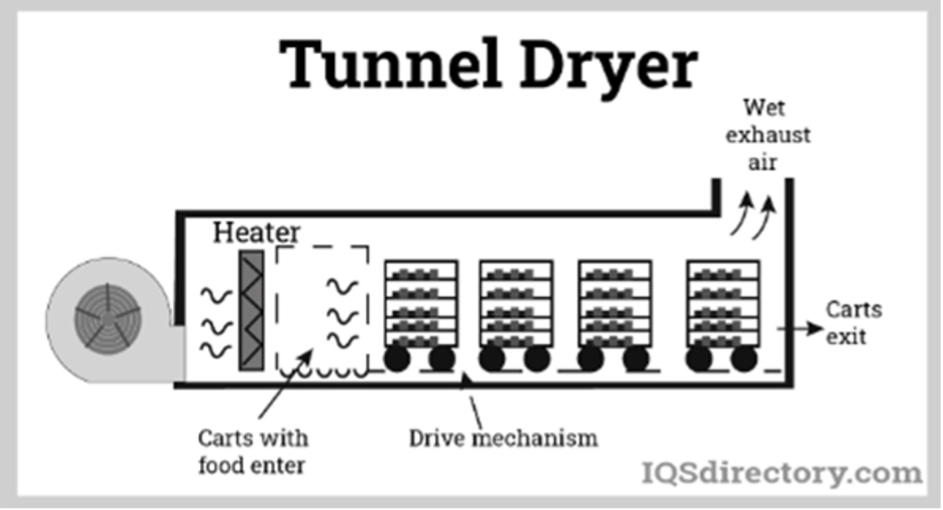
\includegraphics[width=0.8\textwidth]{logos/dryer.png}
    \caption{Tunnel Dryer}
    \label{fig:outlinemindmap}
\end{figure}
\newpage
One can have LCD display to keep track of any errors in the functioning. The
Arduino code for controlling heater is as follows:
\vspace{1cm}
\begin{lstlisting}
# Arduino will only be used if motor speed was found to exceeding the limits to run a fan
#The limits will be found out when material is fulfilled
# Define constants for pin numbers
leftForward = 6
leftBackward = 3
pot = A5

# Initializing some variables
pwm
x

# Running the Setup function once at the beginning
setup() 

  # Set the leftForward and leftBackward as outputs and pot as an input
  pinMode(leftForward , OUTPUT)
  pinMode(leftBackward , OUTPUT)
  pinMode(pot, INPUT)

  # Begin serial communication for debugging
  Serial.begin(9600)

# Loop function to run repeatedly
loop()
  # Reading the analog value from pot
  pwm = analogRead(pot)
  # mapping the value of pwm within appropriate bounds
  x = map(pwm, 0, 1023, 0, 255);
  # Assigning the value of pwm to x, and configuring the values to drive the motor in a particular direction 
  analogWrite(leftForward , x);
  digitalWrite(leftBackward , LOW);
\end{lstlisting}

\href{https://github.com/naunidhsingh03/ELP305-TribeD-Resources/blob/5ba1988fe283faba21ba7098978bb225e509d5cb/Codes/dryer.ino}{\textcolor{blue}{Click here for code reference}}
\newpage

% \clearpage
\begin{figure}[h]
    \centering
    \vspace{0.1cm}
    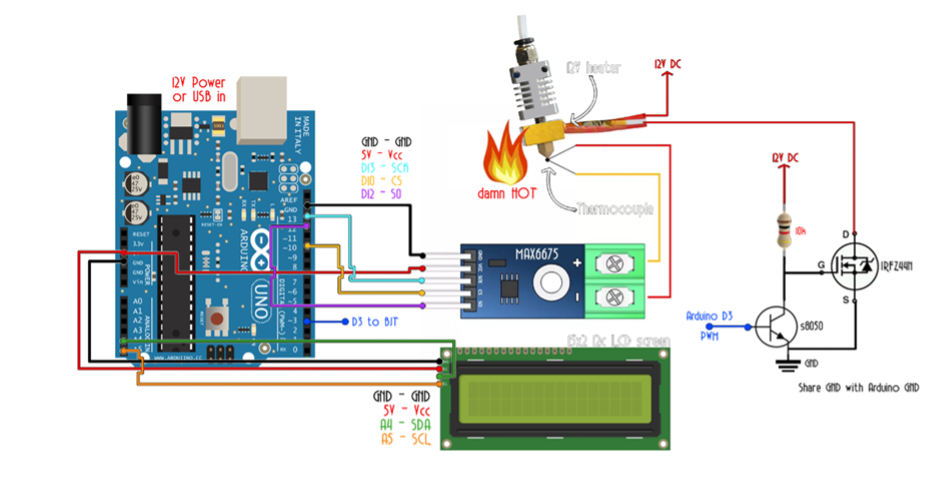
\includegraphics[width=0.8\textwidth]{logos/dryerimgg.png}
    \caption{Control circuit for heater}
    \label{fig:outlinemindmap}
\end{figure}\\
% \vspace{0.5cm}
For running and controlling the blower we need to have an Arduino controlling motor, anemometer, battery, and a bunch of wires.
\begin{figure}[h]
    \centering
    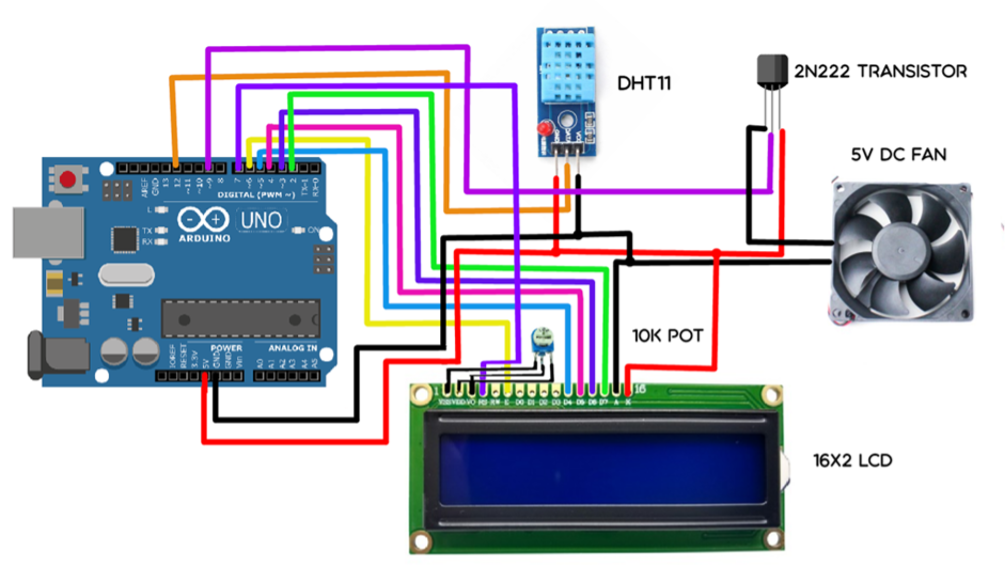
\includegraphics[width=0.8\textwidth]{logos/dryer2img.png}
    \caption{Control Circuit for a DC motor/fan.}
    \label{fig:outlinemindmap}
\end{figure}
% \hspace{1cm}\href{https://github.com/naunidhsingh03/ELP305-TribeD-Resources/blob/b90ebc4b82fa8bee4717be5c5bfab0fe1fc3e671/Codes/dryer_code_2.ino}{\textcolor{blue}{Click here for Code references}}

\newpage

\section{Solvent Research}
Some of the cleansing agents that were researched and tested for oil and grease stains:

\begin{enumerate}
    \item \textbf{\gls{Lipase} \index{Lipase} Enzyme}
    \begin{itemize}[label=$\bullet$]
        \item \textbf{Pros:} Lipase is an enzyme that breaks down oil, making it a potential solution for cleaning oil and grease stains.
        \item \textbf{Cons:} Requires slightly warm water (\textasciitilde40-50\textdegree C) for optimal enzyme action, which may be challenging to maintain.
    \end{itemize}

    \item \textbf{Spot Remover (e.g., Shout) and Hot Water}
    \begin{itemize}[label=$\bullet$]
        \item \textbf{Pros:} Effective in removing both oil and grease stains. Hot water and brushing enhance results.
        \item \textbf{Cons:} Increases energy requirements and costs due to hot water usage. Spot removers add to the overall cost.
    \end{itemize}

    \item \textbf{Spot Lifters (e.g., K2R Spot Lifter) followed by Dry Brushing}
    \begin{itemize}[label=$\bullet$]
        \item \textbf{Pros:} Overcomes the need for scrubbing in hot water. After application, a short waiting period lifts the stain, requiring only brushing in the end.
        \item \textbf{Cons:} Costly \texttt{(\textasciitilde{3300} Rs for 150 ml)} and availability may be an issue for large quantities due to US manufacturing.
    \end{itemize}

    \item \textbf{Baby Powder/Cornstarch/Salt/Vinegar followed by Washing}
    \begin{itemize}[label=$\bullet$]
        \item \textbf{Pros:} Effective in cleaning oil and grease stains significantly.
        \item \textbf{Cons:} Time-consuming, requiring soaking and multiple iterations to remove stains.
    \end{itemize}

    \item \textbf{WD-40 or Lighter Fluid}
    \begin{itemize}[label=$\bullet$]
        \item \textbf{Pros:} Effective in cleaning oil and grease stains significantly.
        \item \textbf{Cons:} Requires 20 minutes of soaking time, and hot water is needed for washing.
    \end{itemize}

    \item \textbf{PCE (Perchloroethylene)}
    \begin{itemize}[label=$\bullet$]
        \item \textbf{Pros:} Nonflammable liquid solvent widely used in dry cleaning, effective in removing oil and grease stains in small quantities.
        \item \textbf{Cons:} Extended exposure to large quantities may cause irritation to eyes, skin, throat, nose, and respiratory system.
    \end{itemize}
    \newpage
    \item \textbf{Handwash (Dettol)}
    \begin{itemize}[label=$\bullet$]
        \item \textbf{Pros:} Biodegradable, environmentally friendly. Can be washed and reused multiple times. Soft and less abrasive.
        \item \textbf{Cons:} May be more prone to staining depending on material and color.
    \end{itemize}

    \item \textbf{Dishwasher (Vim Drop)}
    \begin{itemize}[label=$\bullet$]
        \item \textbf{Pros:} Effective in removing both oil and grease stains by scrubbing with Vim Drop and water with normal pressure.
    \end{itemize}

    \item \textbf{Trichloroethylene (TCE)}
    \begin{itemize}[label=$\bullet$]
        \item \textbf{Pros:} Stain remover and degreaser. Evaporates quickly, leaving behind a dry surface.
        \item \textbf{Cons:} Linked to various health risks, including respiratory, neurological, and reproductive effects. Considered a potential human \index{carcinogen} \gls{carcinogen}. Flammable and persistent in the environment.
    \end{itemize}

    \item \textbf{Isopropyl (Rubbing Alcohol 68-72\%)}
    \begin{itemize}[label=$\bullet$]
        \item \textbf{Pros:} Natural degreasing agent.
        \item \textbf{Cons:} Ineffective in practical experiments on grease and oil-stained cotton cloth. May be effective after longer soaking, making it inefficient due to time constraints.
    \end{itemize}
    \item \textbf{Detergent (Surf Excel)}
    \begin{itemize}[label=$\bullet$]
        \item \textbf{Pros:} Effective on oil stains with slight scrubbing.
        \item \textbf{Cons:} The idea was rejected as it was not effective on grease stains, even after hard scrubbing.
    \end{itemize}
    \item \textbf{Acetone}
    \begin{itemize}[label=$\bullet$]
        \item \textbf{Pros:} As it is volatile, it would be quite convenient in the drying stage.

        \item \textbf{Cons:} We have experimentally seen that it does not work efficiently on grease stains

    \end{itemize}
\end{enumerate}
\newpage

\subsection{Solvent Testing}

% \newpage
\begin{itemize}[label=$\bullet$]
        \item \textbf{WD-40} 
    \end{itemize}
\begin{figure}[h]
    \centering
    \begin{subfigure}{0.37\textwidth}
        \centering
        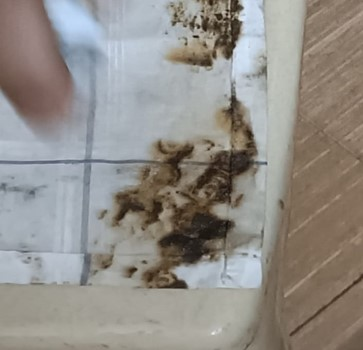
\includegraphics[width=\linewidth]{logos/wd_40_before.jpg}
        \caption{Before}
    \end{subfigure}\hspace{0.1\textwidth}%
    \begin{subfigure}{0.37\textwidth}
        \centering
        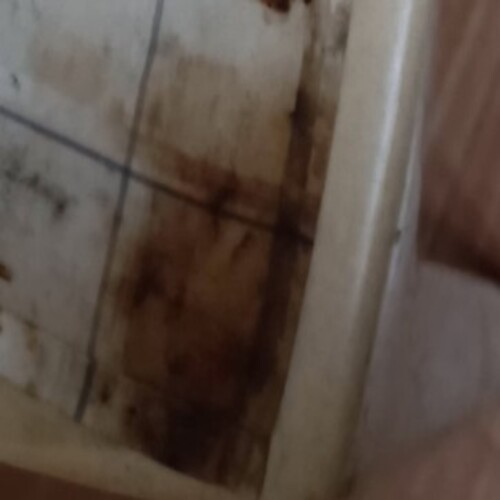
\includegraphics[width=\linewidth]{logos/wd_40_after.jpg}
        \caption{After}
    \end{subfigure}
    \caption{Application of WD-40}
\end{figure}
%\newpage
% \subsection{We tested many solvents and the results are as follows:}
\begin{itemize}[label=$\bullet$]
        \item \textbf{Acetone} 
    \end{itemize}
\begin{figure}[h]
    \centering
    \begin{subfigure}{0.37\textwidth}
        \centering
        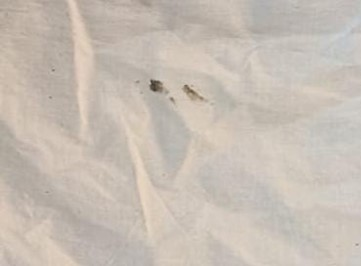
\includegraphics[width=\linewidth]{logos/acetone_before.jpg}
        \caption{Before}
    \end{subfigure}\hspace{0.1\textwidth}%
    \begin{subfigure}{0.37\textwidth}
        \centering
        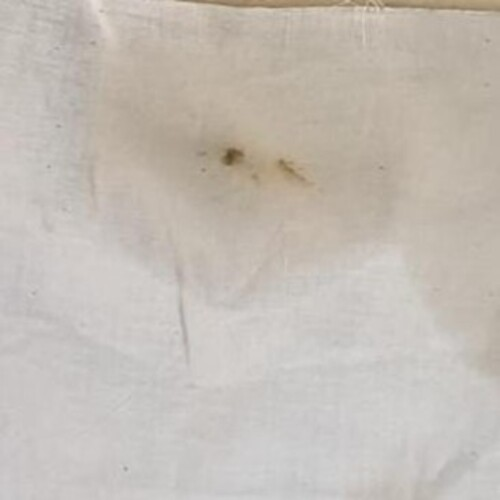
\includegraphics[width=\linewidth]{logos/acetone_after.jpg}
        \caption{After}
    \end{subfigure}
    \caption{Application of Acetone}
\end{figure}
\newpage

\begin{itemize}[label=$\bullet$]
        \item \textbf{Dishwash (Vim)} 
    \end{itemize}
\begin{figure}[h]
    \centering
    \begin{subfigure}{0.37\textwidth}
        \centering
        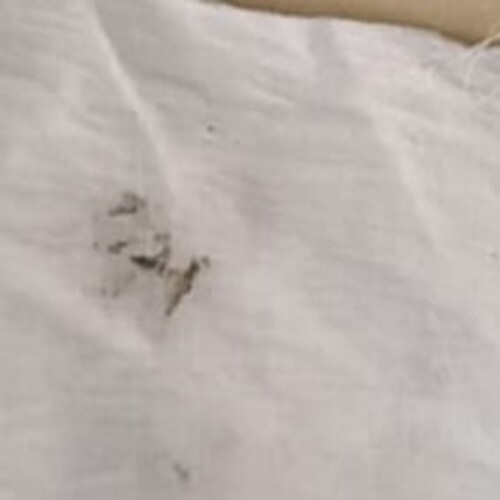
\includegraphics[width=\linewidth]{logos/dishwash_before.jpg}
        \caption{Before}
    \end{subfigure}\hspace{0.1\textwidth}%
    \begin{subfigure}{0.37\textwidth}
        \centering
        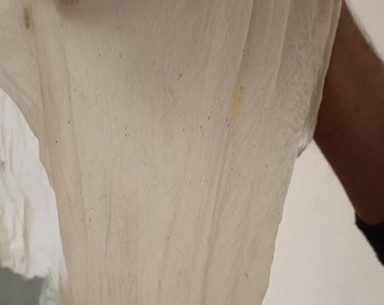
\includegraphics[width=\linewidth]{logos/dishwash_after.jpg}
        \caption{After}
    \end{subfigure}
    \caption{Application of Dishwasher (Vim)}
\end{figure}


% \newpage
\begin{itemize}[label=$\bullet$]
    \item \textbf{Some more applications} 
\end{itemize}
\begin{figure}[h]
    \centering
    \begin{subfigure}{0.37\textwidth}
        \centering
        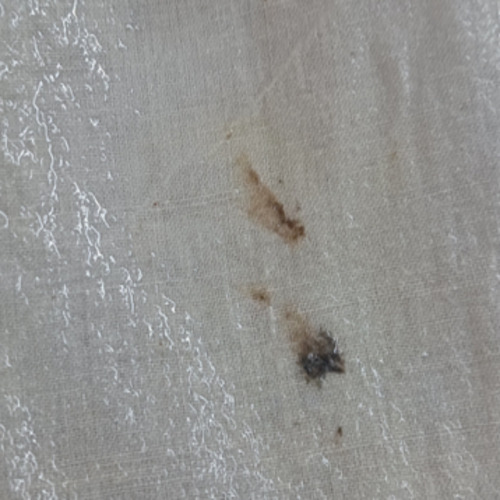
\includegraphics[width=\linewidth]{logos/isopropyl_after.jpg}
        \caption{using Isopropyl}
    \end{subfigure}\hspace{0.1\textwidth}%
    \begin{subfigure}{0.37\textwidth}
        \centering
        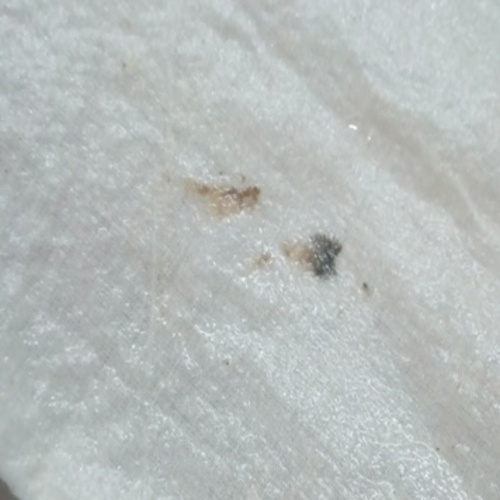
\includegraphics[width=\linewidth]{logos/detergent_after.jpg}
        \caption{using Detergent }
    \end{subfigure}
    \caption{Image of greased cloth after cleaning}
\end{figure}
\newpage

\begin{table}[h]
    \centering
    \vspace{2cm}
    \begin{tabular}{|p{2.5cm}|p{3cm}|p{3cm}|p{3cm}|p{3cm}|}
        
        \hline
        \multicolumn{1}{|c|}{\textbf{Factor}} &  \multicolumn{1}{|c|}{\textbf{Acetone}} &  \multicolumn{1}{|c|}{\textbf{Stain Remover}} &  \multicolumn{1}{|c|}{\textbf{Isopropyl Alcohol}} &  \multicolumn{1}{|c|}{\textbf{Liquid Washing}} \\
        &&&& \textbf{Soap}\\
        \hline
        Suitability for oil-based stains & Excellent & Good & Good & Moderate \\
        \hline
        Amount of solvent & 5-10 mL, test in inconspicuous area first & Follow product instructions (5-15 mL typical) & 5-10 mL, test in inconspicuous area first & Apply directly to stain or dilute 5-10 mL in water for pre-treatment \\
        \hline
        Cleaning time & 5-10 minutes & 10-15 minutes & 5-10 minutes & Depends on washing cycle time \\
        \hline
        Scrubbing intensity & Light scrubbing with soft cloth & Light to moderate scrubbing & Light scrubbing with soft cloth & Moderate scrubbing with brush or hands \\
        \hline
        Evaporation/ drying time & Evaporates quickly (5-10 minutes) & Dries moderately fast (15-30 minutes) & Evaporates quickly (5-10 minutes) & Depends on fabric and drying method \\
        \hline
        Safety & Flammable, use with caution and good ventilation & May contain harsh chemicals, follow product instructions & Flammable, use with caution and good ventilation & Generally safe, but test on inconspicuous area first \\
        \hline
        Fabric suitability & Works well on most fabrics, but test first on delicate fabrics & Check product label for fabric compatibility & Works well on most fabrics, but test first on delicate fabrics & Suitable for washable fabrics \\
        \hline
        
    \end{tabular}
    \caption{Comparison of Different Solvents for Stain Removal}
    \label{tab:solvent_comparison}
\end{table}
% \clearpage
\newpage

\section{Specifications}\label{sec:specs}
\subsection{Energy Specifications}\label{sec:energyspecs}
\begin{table}[h]
    \centering
    
% \centering
\begin{tabular}{|>{\centering\arraybackslash}c|p{7.5cm}|r|}
    

  \hline
  % Content 1 & Content 2 & Content 3 \\
  % \hline
  \multicolumn{1}{|c|}{\multirow{2}{2cm}{\textbf{Roller}}} & Maximum Operating Voltage & 36 V \\
  \cline{2-3} % Horizontal line from second to third column
  \multicolumn{1}{|c|}{} & Maximum Current rating (per channel) & 600 mA \\
  \hline
  % \hline
  \multicolumn{1}{|c|}{\multirow{2}{2cm}{\textbf{Sprinkler}}} & Relay Module Voltage & 5 V \\
  \cline{2-3} % Horizontal line from second to third column
  \multicolumn{1}{|c|}{} & Battery Voltage & 9 V \\
  \cline{2-3}
  \multicolumn{1}{|c|}{} & Water Pump Voltage & 12 V \\
  
  \hline
  % \multicolumn{1}{|c|}{\multirow{6}{2cm}{\textbf{Blower}}} & DC Motor Voltage & 9, 12, 15 V \\
  % \cline{2-3} % Horizontal line from second to third column
  % \multicolumn{1}{|c|}{} & Potentiometer Resistance & 200 $\Omega$ \\
  % \cline{2-3}
  % \multicolumn{1}{|c|}{} & Potentiometer Limiting Element Voltage & 250 V \\
  %   \cline{2-3}
  % \multicolumn{1}{|c|}{} & Battery Power Supply & 9 V \\
  %     \cline{2-3}
  % \multicolumn{1}{|c|}{} & Battery Impedance & 1700 m$\Omega$ \\
  %     \cline{2-3}
  % \multicolumn{1}{|c|}{} & Battery Frequency & 1 KHz \\
  % \hline
    \multicolumn{1}{|c|}{\multirow{1}{2cm}{\textbf{Dryer}}} &  Operating Voltage & 220 V \\
    
  \hline
\end{tabular}
    \caption{Energy specifications for the Model}
    \label{tab:my_label}
\end{table}

% \clearpage

\subsection{Space Specifications}\label{sec:spacespecs}
\begin{table}[h]
\begin{center}
\begin{tabular}{|>{\centering\arraybackslash}c|p{7.5cm}|r|}
    \hline
    \multicolumn{1}{|c|}{\multirow{4}{2cm}{\textbf{Frame} (3mm sheet)}} & Height & 20 cm \\
    \cline{2-3}
  \multicolumn{1}{|c|}{} & Length & 75 cm\\
  \cline{2-3}
  \multicolumn{1}{|c|}{} & Width & 2 cm \\
  \cline{2-3}
  \multicolumn{1}{|c|}{} & Arc radius of the corners & 9 cm \\
  \hline 
  \multicolumn{1}{|c|}{\multirow{3}{2cm}{\textbf{Roller}}} & Height from ground & 21 cm \\
  \cline{2-3}
  \multicolumn{1}{|c|}{} & Length & 30 cm \\
  \cline{2-3}
  \multicolumn{1}{|c|}{} & Diameter & 8 cm \\
  \hline
  \multicolumn{1}{|c|}{\multirow{3}{2cm}{\textbf{Box}}} & Length & 75 cm \\
  \cline{2-3}
  \multicolumn{1}{|c|}{} & Height & 10 cm \\
  \cline{2-3}
  \multicolumn{1}{|c|}{} & width & 30 cm \\
  \hline 
  \multicolumn{1}{|c|}{\multirow{3}{2cm}{\textbf{Wall}}} & Height & 20 cm \\
  \cline{2-3}
  \multicolumn{1}{|c|}{} & Length & 75 cm \\
  \cline{2-3}
  \multicolumn{1}{|c|}{} & Width & 30 cm \\
  \hline 
  \multicolumn{1}{|c|}{\multirow{2}{2cm}{\textbf{Scrubber}}} & Length & 18 cm \\
  \cline{2-3}
  \multicolumn{1}{|c|}{} & Width & 3 cm\\
  
  \hline 
  \multicolumn{1}{|c|}{\multirow{1}{2cm}{\textbf{Fan}}} & Diameter & 3 inches\\
  \hline
\end{tabular}
\caption{Space specifications for the Model}
\end{center}
\end{table}

\clearpage

\subsection{Power Specifications}\label{sec:powspecs}
\begin{table}[h]
\begin{center}
\begin{tabular}{|>{\centering\arraybackslash}c|p{7.5cm}|r|}
\hline
\multicolumn{1}{|c|}{\multirow{1}{2cm}{\textbf{Roller}}} & Power Rating & 21.6 W \\
    \hline
\multicolumn{1}{|c|}{\multirow{1}{2cm}{\textbf{Sprinkler}}} & Power Rating & 18 W \\
    \hline
% \multicolumn{1}{|c|}{\multirow{4}{2cm}{\textbf{Blower}}} &     DC Motor Power  & 300 W \\
%     \cline{2-3}
%     \multicolumn{1}{|c|}{} & DC Motor Speed  & 7000 RPM \\
%     \cline{2-3}
%     \multicolumn{1}{|c|}{} & BC547 Max collector Dissipation   & 1.5 W \\
%     \cline{2-3}
%     \multicolumn{1}{|c|}{} & Resistor (100 M$\Omega$) Power Rating  & 0.25 - 0.5 W \\
%     \hline
\multicolumn{1}{|c|}{\multirow{2}{2cm}{\textbf{Dryer}}} & 
 Actual machine requirement & 4-6 KW \\
    \cline{2-3}
    \multicolumn{1}{|c|}{} & For Prototype & 1 - 2 KW \\
    \hline
\end{tabular}
\caption{Power specifications for the Model}
\end{center}
    \end{table}

% \clearpage
\subsection{Cost Specifications}\label{sec:costspecs}

\begin{table}[h]
\begin{center}
\begin{tabular}{|>{\centering\arraybackslash}c|p{7.5cm}|r|}
    \hline
    \multicolumn{1}{|c|}{\multirow{1}{2cm}{\textbf{Roller}}} & Prototype Average Cost & 200 INR \\
    \hline

\multicolumn{1}{|c|}{\multirow{8}{2cm}{\textbf{Sprinkler}}} & Arduino & 2500 INR \\
    \cline{2-3}
    \multicolumn{1}{|c|}{} & \gls{Nozzle} & 500 INR \\
    \cline{2-3}
    \multicolumn{1}{|c|}{} & Resistors & 1 - 2 INR \\
   \cline{2-3}
    \multicolumn{1}{|c|}{} & Breadboard & 90 INR \\
    \cline{2-3}
    \multicolumn{1}{|c|}{} & Relay Module & 50 INR \\
    \cline{2-3}
    \multicolumn{1}{|c|}{} & Connecting Wires & 15 INR \\
    \cline{2-3}
    \multicolumn{1}{|c|}{} & Pipe (2-3 meters) & 200 INR \\
    \cline{2-3}
    \multicolumn{1}{|c|}{} & Solvent Pump & 200 INR \\
    \hline
\multicolumn{1}{|c|}{\multirow{2}{2cm}{\textbf{Scrubber}}} & Cost per meter & 300-400 INR \\
    \cline{2-3}
    \multicolumn{1}{|c|}{} & No of scrubbers & 2 - 4 \\
    \hline
% \multicolumn{1}{|c|}{\multirow{6}{2cm}{\textbf{Blower}}} & Arduino & 2550 INR \\
%     \cline{2-3}
%     \multicolumn{1}{|c|}{} & Resistor(100 $\Omega$) & 1 INR \\
%     \cline{2-3}
%     \multicolumn{1}{|c|}{} & Transistor & 1 INR \\
%     \cline{2-3}
%     \multicolumn{1}{|c|}{} & Potentiometer & 17 INR \\
%     \cline{2-3}
%     \multicolumn{1}{|c|}{} & 9 V battery & 300 INR \\
%     \cline{2-3}
%     \multicolumn{1}{|c|}{} & DC Motor & 260 INR \\
%     \hline
\multicolumn{1}{|c|}{\multirow{2}{2cm}{\textbf{Dryer}}} & Actual Machine Cost & 1,00,000 INR \\
    \cline{2-3}
    \multicolumn{1}{|c|}{} & Prototype cost & 800 INR \\
    \hline
\end{tabular}
\caption{Cost specifications for the Model}
\end{center}
\end{table}
\clearpage
\subsection{Performance Specifications}\label{sec:perfspecs}
    \subsubsection*{Roller}
        \begin{itemize}[label=$\bullet$]
        \item Rolling Capacity: $\sim$60-80 meters/min.
    \item Rewind Diameter: 1.8-2 meters.
    \item The driver module for the prototype can be used simultaneously by other motors in the system.
    \item The cost of the actual machine can be reduced significantly because it would be integrated with other components.
    \item If a small DC motor is used, a no-load speed of $\sim$9000 rpm, and a loaded speed of $\sim$5000 rpm can be achieved in the prototype. 
        \end{itemize}
    \subsubsection*{Soap Water Sprinkler}
        \begin{itemize}[label=$\bullet$]
        \item HCSR04 Ultrasonic Sensor will check if there is any object placed before the dispenser. A solenoid valve will be used to control the flow of water by energising and deenergising. 
        \item Arduino controls the operation of the water pump. It also controls the flow rate and directions of water.
        \end{itemize}
    \subsubsection*{Scrubber}
        \begin{itemize}[label=$\bullet$]
        \item Stationary scrubbers/brushes remain fixed during operation, providing a stable cleaning surface. 
        \item The static design allows for controlled and targeted cleaning of fabrics, ensuring uniform and effective removal of dirt and contaminants. 
        \end{itemize}
    % \subsubsection*{Blower}
    %     \begin{itemize}[label=$\bullet$]
    %     \item \gls{Control Mechanism}: \index{Control Mechanism} Potentiometer for DC motor speed control 
    %     \item Efficiency: Improved motor control using a transistor to prevent overloading and overheating 
    %     \item Lifespan: Enhanced motor lifespan due to efficient control using the transistor 
    %     \item \gls{Compatibility}:\index{Compatibility} Multiple DC motors can be connected with slight wiring modifications 
    %     \end{itemize}
    \subsubsection*{Dryer}
        \begin{itemize}[label=$\bullet$]
        \item Control Mechanism: Arduino, a temperature sensor (thermocouple), a relay module, battery and bunch of connecting wires will be used 
        \item \gls{Efficiency}:  \index{Efficiency} Most efficient counter current configuration will be used 
        \item Power requirements will be optimized on the basis of mathematical modelling and simulations done to observe the humidity content with rate of air flow and power input to heater and blower 
        \end{itemize}
        \clearpage
\subsection{Manpower Specifications}\label{sec:mpspecs}
\begin{table}[h]
\begin{center}
\begin{tabular}{|p{8cm}|r|}

    \hline
    \textbf{Team} & \textbf{Man Hours} \\
    \hline
    Research Team & 82 Hours \\
    \hline
    Electrical Team & 60 Hours \\
    \hline
    Fabrication Team & 13.5 Hours \\
    \hline
    Documentation Team & 127 Hours \\
    \hline
    Consultant & 2 Hours \\
    \hline
\end{tabular}
\caption{Manpower specifications for the Machine}
\end{center}
\end{table}
\begin{figure}[h]
    \centering
    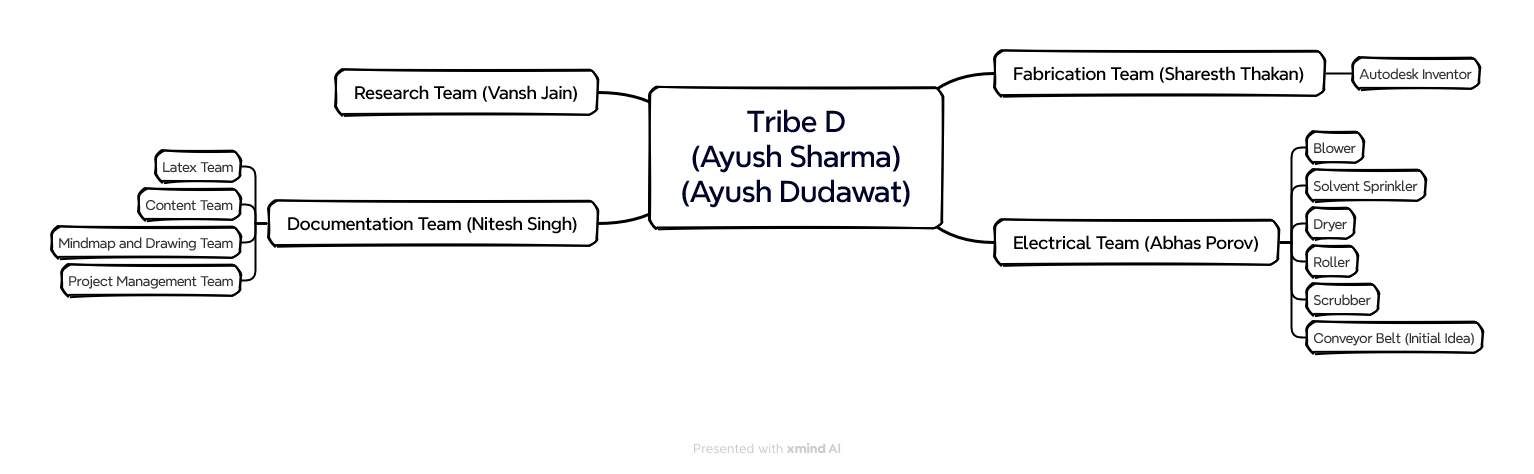
\includegraphics[width=1.1\textwidth]{logos/P1_WorkDist_TribeD_MindMap_L3.png}
    \caption{Work distribution mind map}
    \label{fig:specsmindmap}
\end{figure}

\subsection{Milestone Specifications}\label{sec:msspecs}

\subsubsection*{Phase 1 (25 marks) (25\% completed)}
\begin{enumerate}
    \item[1.] Outline and ideation of the initial design based on the initial requirements of the client. Discussion of the initial design with the whole team, looking for solutions to the loopholes suggested by the team to make it feasible in the real world. (6 marks)

    \item[2.] Empirical research on various solvents and cleaning agents like isopropyl alcohol, WD40, acetone, dishwashing liquid (vim drop), detergent, and vanish stain remover by application on the cloth, and finalizing the best solvent. (6 marks)

    \item[3.] Scraping of the previous idea due to some last-minute changes and ideation of the new design based on the revised requirements of the client. (6 marks)

    \item[4.] Validation of our idea with Fabrication and Electrical Teams and making on-site visits to find facilities to build our final product. (4 marks)

    \item[5.] Discussion of the new idea with the consultant and incorporating the changes suggested by them to finalise the idea. (3 marks)
    
\end{enumerate}
\textbf{TRL 2:} Outlining the proposed design, learning skills, and formation of a team indicates the initiation of the project. The use of AutoCAD for basic visualization enhances the maturity by translating ideas into tangible forms, although it's still in the early stages of development involving ideation and conceptualization.

\vspace{0.5cm}
\subsubsection*{Phase 2 (25 marks) (50\% completed)}
\begin{enumerate}
    \item[1.] Realisation of the components required in the design by using a basic CAD model incorporating specifics such as dimensions and placement of every minor component within the model Incorporating information about the dimensions and positions of all the minor components within the model - (10 marks).\newline
    \newline
    Frame is curved from corners with arc radius = 9cm for smooth flow of cloth over it.
    \begin{table}[h]
\begin{center}
\begin{tabular}{|>{\centering\arraybackslash}c|p{7.5cm}|r|}
    \hline
    \multicolumn{1}{|c|}{\multirow{4}{2cm}{\textbf{Frame} (3mm sheet)}} & Height & 20 cm \\
    \cline{2-3}
  \multicolumn{1}{|c|}{} & Length & 75 cm\\
  \cline{2-3}
  \multicolumn{1}{|c|}{} & Width & 2 cm \\
  \cline{2-3}
  \multicolumn{1}{|c|}{} & Arc radius of the corners & 9 cm \\
  \hline 
  \multicolumn{1}{|c|}{\multirow{3}{2cm}{\textbf{Roller}}} & Height from ground & 21 cm \\
  \cline{2-3}
  \multicolumn{1}{|c|}{} & Length & 30 cm \\
  \cline{2-3}
  \multicolumn{1}{|c|}{} & Diameter & 8 cm \\
  \hline
  \multicolumn{1}{|c|}{\multirow{3}{2cm}{\textbf{Box}}} & Length & 75 cm \\
  \cline{2-3}
  \multicolumn{1}{|c|}{} & Height & 10 cm \\
  \cline{2-3}
  \multicolumn{1}{|c|}{} & width & 30 cm \\
  \hline 
  \multicolumn{1}{|c|}{\multirow{3}{2cm}{\textbf{Wall}}} & Height & 20 cm \\
  \cline{2-3}
  \multicolumn{1}{|c|}{} & Length & 75 cm \\
  \cline{2-3}
  \multicolumn{1}{|c|}{} & Width & 30 cm \\
  \hline 
  \multicolumn{1}{|c|}{\multirow{2}{2cm}{\textbf{Scrubber}}} & Length & 18 cm \\
  \cline{2-3}
  \multicolumn{1}{|c|}{} & Width & 3 cm\\
  
  \hline 
  \multicolumn{1}{|c|}{\multirow{1}{2cm}{\textbf{Fan}}} & Diameter & 3 inches\\
  \hline
\end{tabular}
\caption{Dimensions of the Model}
\end{center}
\end{table}
\newpage
    \item[2.] Conducting trial and error checks on the code and activating the motors through iterative testing to ensure precise and effective control over the motorised components.(8 marks)
    \item[3.] Finalising the items required for building the prototype model and sending the procurement list to the vendor. (7 marks)
    % \item[4.] Testing the chemicals used on the cloth.
    % \item[5.] Finalized design of the visualized model using FreeCAD.
\end{enumerate}
\textbf{TRL 3:} Realizing components, conducting trial and error checks on the code, purchasing required materials, and finalizing the design using ‘FreeCAD’ signify a transition from the early stages to a more mature state. The culmination of these activities indicates a significant advancement in technology readiness, approaching the stage where it can be practically implemented.

\vspace{1cm}
\subsubsection*{Phase 3 (25 marks) (75\% completed)}
\begin{enumerate}

    \item[1.] Concluding the circuits and codes for the components.(5 marks)
    \item[2.] Individual Component realisation (20 marks)
\end{enumerate}

\begin{table}[h]
\begin{center}
\begin{tabular}{|p{3cm}|p{10cm}|r|}
\hline
    \multicolumn{1}{|c|}{\textbf{Components}} & \multicolumn{1}{|c|}{\textbf{Specifications}} & \multicolumn{1}{|c|}{\textbf{Marks}} \\
\hline
Rollers (2 in number) & Both move clockwise (at the same speed to keep the cloth taut at all times) one to unroll the cloth towards the machine and the other to roll the cloth onto itself after the cleaning process & 2 \\
\hline
DC BO Motors operation (3 in number) & To control the rotation of rollers and the cloth at constant speed & 3 \\
\hline
Main frame & The cloth comes from the roller, hangs on it and falls on either side &	3 \\
\hline
Water sprinkler & Aquarium pipes ooze out water onto the edges of the cloth. & 0.5\\
\hline
Soap sprinklers	& Located just above the scrubbers, they are similar to water sprinklers but ooze out soap solution instead. & 0.5 \\
\hline
Solvent Dispenser and water pump operation & To control the dispensing of water and soap from sprinklers, it is essential to regulate the operation of the pumps using an Arduino controlled circuit.	& 3 \\
\hline

% \hline
\end{tabular}
\caption{Marks distribution for Phase 3}
\end{center}
\end{table}

\clearpage
\begin{table}[h]
\begin{center}
\begin{tabular}{|p{3cm}|p{10cm}|p{1.8cm}|}
\hline
Scrubber (4 in number, 2 on each side)	& The scrubbers are placed close to the main frame with gaps between them. They are stationary and the moving cloth’s edges rub past it (against the middle part), thus cleaning them. & 1 \\
\hline
Fans (2 in number, 1 on each side) & Constituting the final step, they are placed at a fair distance from the middle part, so as to not rip the cloth off, but dry the cloth to finally roll it back up. & 1\\
\hline
DC 555 Motor operation (3 in number) & To regulate the operation of the dryer motors (fans), ensuring efficient flow of air onto the fabric for effective drying.& 2 \\
\hline
Tub	& Placed under the machine in the section of water and soap sprinklers, to collect the water and drain it off. & 1 \\
\hline
Water and soap solution tanks(bucket) & The water and soap sprinklers take respective solution from this to sprinkle on the cloth. & 1 \\
\hline
Zero Board & Realisation of the circuits used in controlling the electrical components of the prototype by making the essential connections through soldering. & 2 \\
\hline

\end{tabular}
\caption{Marks distribution for Phase 3}
\end{center}
\end{table}

\textbf{TRL 4:} Demonstrating fully functional components to the client, finalizing circuits and codes, and providing detailed specifications represent a high level of maturity. This milestone is marked by a readiness for deployment, with working components and comprehensive documentation that can lead to the assembly of a full prototype.

\subsubsection*{Phase 4 (25 marks) (100\% completed)}
% \begin{enumerate}
\begin{enumerate}[label=\arabic*.]
    \item  Assembling all the different components to make a full working \index{prototype} \gls{prototype}.(9 marks)
    \item  The following things can be expected to be assured in the model:(8 marks)
    \begin{enumerate}[label=\alph*.]
        \item For the CAD model-(4 marks)
        \begin{enumerate}[label=\roman*.]
            \item A detailed CAD model on Autodesk Inventor showing positioning of the parts of the fabric-cleaning machine.(2 marks)
            \item Circuits showing a general idea of where and how the motors and other components are included.(2 marks)
            \end{enumerate}
        \item Fabrication assurances -(4 marks)
        \begin{enumerate}[label=\roman*.]
           \item Ensuring the seamless operation of all components, such as \index{scrubber} \gls{scrubber} and rollers, in the \index{prototype} \gls{prototype} model designed for uninterrupted cloth processing.
           \end{enumerate}
        \end{enumerate}
\newpage
\item Listing out electrical limitations -
    \begin{enumerate}[label=\alph*.]
        \item As motors necessitate a direct current \gls{current} (DC) power supply, we will employ a regulated power supply to demonstrate the functionality of our prototype.
        \item Considering that the electrical connections are not very complicated and do not demand the use of a printed circuit board (PCB), we plan to implement the circuit using a zero board and establish the essential connections through soldering.
        \item To achieve proper working of DC motors, a requisite power supply voltage not exceeding 12 volts is necessary, along with conductive wires having a current rating of 2 A.
        \end{enumerate}
        
\item Prototype Limitation-
The expected cloth obtained after undergoing the process is not sufficiently dry due to the use of cold air blowers rather than hot air owing to the length/power constraints.
\item Conducting a live demonstration for the client using a sample cloth with edges stained with oil and grease to simulate a just-manufactured cotton cloth, followed by an assessment of the model's performance based on the quality of cleaning. (8 marks)

\end{enumerate}

\textbf{TRL 5:} Assembling all components into a working \index{prototype} \gls{prototype}, conducting a live demonstration using a sample cloth, and assessing performance in real-world conditions with actual stains indicate a high level of readiness for practical application and deployment. The technology has progressed to the point where it can be reliably demonstrated and evaluated in real-world scenarios, signalling a mature state.
% \section{Design}\label{sec:design}
% \section{Closure}\label{sec:closure}
% \section{Reuse}\label{sec:reuse}
% \end{section{Reuse}}
\newline
\rule{\linewidth}{0.5pt}
\newpage

\newpage
\pagestyle{plain}
\pagenumbering{alph}
\section*{List of Tables}\phantomsection\label{sec:listoftables} 
\addcontentsline{toc}{section}{List of Tables}
\renewcommand{\listtablename}{}
\listoftables

\newpage
\pagestyle{plain}
\section*{List of Figures}\phantomsection\label{sec:listoffigures}
\addcontentsline{toc}{section}{List of Figures}
\renewcommand{\listfigurename}{}

\listoffigures

\newpage
\pagestyle{plain}
\section*{Abbreviations}\phantomsection\label{sec:abbrevations}
\addcontentsline{toc}{section}{Abbreviations}
   \begin{table}[h]
      \centering
      \begin{tabular}{|c|>{\centering\arraybackslash}p{8cm}|}
        \hline
        \textbf{Abbreviation} & \textbf{Stands For} \\
        \hline
        IF & Involvement Factor \\
        \hline
        ID & Identification \\
        \hline
        CPCB & Central Pollution Control Board \\
        \hline
        mg & Milligram \\
        \hline
        AC & Alternating Current \\
        \hline
        dB & Decibals \\
        \hline
        Kg & Kilograms \\
        \hline
        ABS & Acrylonitrile Butadiene Styrene \\
        \hline
        PWM & Pulse Width Modulation \\
        \hline
        IC & Integrated Circuits \\
        \hline
        PCE & perchloroethylene \\
        \hline
        TCE & Trichloroethylene \\
        \hline
        TRL & Technology Readiness Level \\
        \hline
        CAD & Computer Aided Design \\
        \hline
        NMOS & N-type Metal-Oxide-Semiconductor
 \\
        \hline
        LED & Light Emitting Diode \\
        \hline
        TCE & Tri-Chloro-Ethane \\
        \hline
        PCE & Power Conversion Efficiency \\
        \hline
      \end{tabular}
      \caption{Abbreviations}
      \label{tab:abbreviations}
    \end{table}
% \section{Index}\label{sec: indexredirect}
% \hyperref[sec:myindex]{$\bullet$ Click here to go to the Index}\hfill \pageref{sec: myindex}

% \section{Glossary}\label{sec: glossaryredirect}
% \hyperref[sec: glossary]{$\bullet$ Click here to go to the Glossary}\hfill \pageref{sec: glossary}
\newpage



\section*{Our Tribe}\phantomsection\label{sec:ourtribeone}
\pagestyle{plain}
\addcontentsline{toc}{section}{Our Tribe}
\begin{table}[h]
\centering
  \caption{Team Members list 1}
  \label{tab:team-members}
    \rowcolors{2}{white}{lightergray}
  
  % \begin{tabular}{|p{.5cm}|p{3cm}|>{\raggedleft}p{2.7cm}|p{2.58cm}|>{\raggedleft}p{5.8cm}|p{0.3cm}|}
  \begin{tabular}{|>{\raggedleft}p{.5cm}|>{\raggedright}p{2.9cm}|r|>{\raggedleft}p{2.8cm}|r|p{.4cm}|}
\hline
SNo. & \multicolumn{1}{|c|}{Name} & \multicolumn{1}{|c|}{Roll No.} & \multicolumn{1}{|c|}{Position} & \multicolumn{1}{|c|}{Email} & \multicolumn{1}{|c|}{IF} \\
\hline
\rowcolor{lightgray}
1 & \href{https://www.linkedin.com/in/ayush-dudawat-6b7a9b222/}{Ayush Dudawat} & 2021EE10694 & Tribe Coordinator & \href{mailto:ee1210694@ee.iitd.ac.in}{\nolinkurl{ee1210694@ee.iitd.ac.in}} & 1 \\ 
\rowcolor{lightgray}
2 & \href{https://www.linkedin.com/in/ayush-sharma-b01346224/}{Ayush Sharma} & 2021MT10244 & Tribe Coordinator &
\href{mailto:mt1210244@maths.iitd.ac.in}{\nolinkurl{mt1210244@maths.iitd.ac.in}} & 1 \\
\rowcolor{lightergray}
3 & \href{https://www.linkedin.com/in/nitesh-singh-a79a17223/}{Nitesh Singh} & 2021MT10250 & Documentation Coordinator &
\href{mailto:mt1210250@maths.iitd.ac.in}{\nolinkurl{mt1210250@maths.iitd.ac.in}} & 1 \\
\rowcolor{lightergray}
4 & \href{https://www.linkedin.com/in/vansh-jain-36569b225/}{Vansh Jain} & 2021MT10234 & Research Coordinator &
\href{mailto:mt1210234@maths.iitd.ac.in}{\nolinkurl{mt1210234@maths.iitd.ac.in}} & 1 \\
\rowcolor{lightergray}
5 & \href{https://www.linkedin.com/in/sharesth-thakan-249504250/}{Sharesth Thakan} & 2021EE30730 & Fabrication and Testing Coordinator & \href{mailto:ee3210730@ee.iitd.ac.in}{\nolinkurl{ee3210730@ee.iitd.ac.in}} & 1 \\
\rowcolor{lightergray}
6 & \href{https://www.linkedin.com/in/abhas-porov-b69077248/}{Abhas Porov} & 2021EE10781 & Electrical and Simulation Coordinator &
\href{mailto:ee1210781@ee.iitd.ac.in}{\nolinkurl{ee1210781@ee.iitd.ac.in}} & 1 \\
\hline
7 & \href{https://www.linkedin.com/in/tanisha-jangra-5203132ab}{Tanisha} & 2021MT10927 & Research &
\href{mailto:mt1210927@maths.iitd.ac.in}{\nolinkurl{mt1210927@maths.iitd.ac.in}} & 0.6 \\
8 & \href{https://www.linkedin.com/in/shreyansh-jain-6abb9124b/}{Shreyansh Jain} & 2021MT10930 & Research &
\href{mailto:mt1210930@maths.iitd.ac.in}{\nolinkurl{mt1210930@maths.iitd.ac.in}} & 0.8 \\
9 & \href{https://www.linkedin.com/in/rishika-arya-266082279/}{Rishika Arya} & 2021MT10926 & Research &
\href{mailto:mt1210926@maths.iitd.ac.in}{\nolinkurl{mt1210926@maths.iitd.ac.in}} & 1 \\
10 & \href{https://www.linkedin.com/in/sarmistha-subhadarshini-507172243}{Sarmistha} & 2021MT10261 & Research &
\href{mailto:mt1210261@maths.iitd.ac.in}{\nolinkurl{mt1210261@maths.iitd.ac.in}} & 1 \\
11 & \href{https://www.linkedin.com/in/anshika-prajapati-9b855022b/}{Anshika Prajapati} & 2021MT60961 & Research &
\href{mailto:mt6210961@maths.iitd.ac.in}{\nolinkurl{mt6210961@maths.iitd.ac.in}} & 1 \\
12 & \href{https://www.linkedin.com/in/rupam-kumawat-b27949253/}{Rupam Kumawat} & 2021MT60267 & Research &
\href{mailto:mt6210267@maths.iitd.ac.in}{\nolinkurl{mt6210267@maths.iitd.ac.in}} & 1 \\
13 & \href{www.linkedin.com/in/sakshimagarkar/}{Sakshi Magarkar} & 2021MT60965 & Research & \href{mailto:mt6210965@maths.iitd.ac.in}{\nolinkurl{mt6210965@maths.iitd.ac.in}} & 1 \\
14 & \href{https://www.linkedin.com/in/aniket-pandey-b5b9a1263/}{Aniket Pandey} & 2021MT60266 & Research & \href{mailto:mt6210266@maths.iitd.ac.in}{\nolinkurl{mt6210266@maths.iitd.ac.in}} & 1 \\
15 & \href{https://www.linkedin.com/in/nancy-kansal-1b5384234/}{Nancy Kansal} & 2021MT10905 & Research & \href{mailto:mt1210905@maths.iitd.ac.in}{\nolinkurl{mt1210905@maths.iitd.ac.in}} & 1 \\
16 & \href{https://www.linkedin.com/in/divyansh-agarwal-22989525b/}{Diyvansh Agarwal} & 2021EE10035 & Research & \href{mailto:ee1210035@ee.iitd.ac.in}{\nolinkurl{ee1210035@ee.iitd.ac.in}} & 0.9 \\
17 & \href{https://www.linkedin.com/in/mukund-aggarwal}{Mukund Aggarwal} & 2021MT60939 & Research & \href{mailto:mt6210939@maths.iitd.ac.in}{\nolinkurl{mt6210939@maths.iitd.ac.in}} & 1 \\
\hline
\end{tabular}

\end{table}
\begin{table}[h]\label{sec:ourtribetwo}
\centering
  \caption{Team Members list 2}
  % \label{tab:team-members}
    \rowcolors{2}{white}{lightergray}
  \begin{tabular}{|>{\raggedleft}p{.5cm}|>{\raggedleft}p{2.9cm}|r|>{\raggedleft}p{2.8cm}|r|p{.4cm}|}
  \hline
18 & \href{https://www.linkedin.com/in/tanishk-singh-80ba09224/}{Tanishk Singh} & 2021EE10167 & Research & \href{mailto:ee1210167@ee.iitd.ac.in}{\nolinkurl{ee1210167@ee.iitd.ac.in}} & 0.6 \\
19 & \href{https://www.linkedin.com/in/akshansh-rajora-5794b5228}{Akshansh Rajora} & 2021MT10933 & Research & \href{mailto:mt1210933@maths.iitd.ac.in}{\nolinkurl{mt1210933@maths.iitd.ac.in}} & 0.6 \\
20 & \href{https://www.linkedin.com/in/ayush-madhur-40a575236/}{Ayush Madhur}& 2021EE10161 & Research & \href{mailto:ee1210161@ee.iitd.ac.in}{\nolinkurl{ee1210161@ee.iitd.ac.in}} & 0.6 \\
21 &\href{https://www.linkedin.com/in/keshvi-tomer-4b0331236/}{Keshvi Tomar} & 2021EE10682 & Research & \href{mailto:ee1210682@ee.iitd.ac.in}{\nolinkurl{ee1210682@ee.iitd.ac.in}} & 0.9 \\
22 & \href{https://www.linkedin.com/in/kanak-kumar-538ab2247/}{Kanak Kumar Singh} & 2021EE10163 & Research & \href{mailto:ee1210163@ee.iitd.ac.in}{\nolinkurl{ee1210163@ee.iitd.ac.in}} & 0.6 \\
23 & \href{https://www.linkedin.com/in/aravind-udupa-266a52223/}{Aravind Udupa} & 2021MT60940 & Research & \href{mailto:mt6210940@maths.iitd.ac.in}{\nolinkurl{mt6210940@maths.iitd.ac.in}} & 1 \\
24 & \href{https://www.linkedin.com/in/arpit-rathore-56b535223/}{Arpit Rathore} & 2021MT10920 & Research & \href{mailto:mt1210920@maths.iitd.ac.in}{\nolinkurl{mt1210920@maths.iitd.ac.in}} & 1 \\
\hline
25 & \href{https://www.linkedin.com/in/vandit-srivastava}{Vandit Srivastava} & 2021EE10640 & Electrical & \href{mailto:ee1210640@ee.iitd.ac.in}{\nolinkurl{ee1210640@ee.iitd.ac.in}} & 1 \\
26 & \href{https://www.linkedin.com/in/ankita-meena-2b919a236/}{Ankita Meena} & 2021EE10173 & Electrical & \href{mailto:ee1210173@ee.iitd.ac.in}{\nolinkurl{ee1210173@ee.iitd.ac.in}} & 1 \\
27 & \href{https://www.linkedin.com/in/aditya-gupta-178638228}{Aditya Gupta} & 2021EE30713 & Electrical & \href{mailto:ee3210713@ee.iitd.ac.in}{\nolinkurl{ee3210713@ee.iitd.ac.in}} & 1 \\
28 & \href{https://www.linkedin.com/in/aditya-bhalotia-756654253}{Aditya Bhalotia} & 2021EE30698 & Electrical & \href{mailto:ee3210698@ee.iitd.ac.in}{\nolinkurl{ee3210698@ee.iitd.ac.in}} & 1 \\
29 & \href{https://www.linkedin.com/in/ayush-shrivastava-264398248}{Ayush Shrivastava} & 2021EE10632 & Electrical & \href{mailto:ee1210632@ee.iitd.ac.in}{\nolinkurl{ee1210632@ee.iitd.ac.in}} & 1 \\
30 & \href{https://www.linkedin.com/in/harshit-nagar-178a33253}{Harshit Nagar} & 2021EE10155 & Electrical & \href{mailto:ee1210155@ee.iitd.ac.in}{\nolinkurl{ee1210155@ee.iitd.ac.in}} & 1 \\

31 & \href{www.linkedin.com/in/shreyansh-jaiswal-4b79b2228}{Shreyansh Jaiswal} & 2021EE10154 & Electrical & \href{mailto:ee1210154@ee.iitd.ac.in}{\nolinkurl{ee1210154@ee.iitd.ac.in}} & 1 \\
32 & \href{https://www.linkedin.com/in/akshar-tripathi-9a267425b/}{Akshar Tripathi} & 2021EE10980 & Electrical & \href{mailto:ee1210980@ee.iitd.ac.in}{\nolinkurl{ee1210980@ee.iitd.ac.in}} & 1 \\
33 & \href{https://www.linkedin.com/in/muskan-yadav-2b0651b4}{Muskan Yadav} & 2021EE10686 & Electrical & \href{mailto:ee1210686@ee.iitd.ac.in}{\nolinkurl{ee1210686@ee.iitd.ac.in}} & 1 \\
34 & \href{https://www.linkedin.com/in/pavan-bharadwaj-07025a281/}{Pavan Bharadwaj} & 2021EE10630 & Electrical & \href{mailto:ee1210630@ee.iitd.ac.in}{\nolinkurl{ee1210630@ee.iitd.ac.in}} & 1 \\
35 & \href{https://www.linkedin.com/in/mokshavi-reddy-93b41a255}{Aluka Mokshavi} & 2021MT10909 & Electrical & \href{mailto:mt1210909@maths.iitd.ac.in}{\nolinkurl{mt1210909@maths.iitd.ac.in}} & 1 \\
36 & \href{https://www.linkedin.com/in/sathvika-palle-28a13025a}{Palle Sathvika} & 2021MT10928 & Electrical & \href{mailto:mt1210928@maths.iitd.ac.in}{\nolinkurl{mt1210928@maths.iitd.ac.in}} & 1 \\
37 & \href{www.linkedin.com/in/shubham-anand-055423252}{Shubham Anand} & 2021EE10674 & Electrical & \href{mailto:ee1210674@ee.iitd.ac.in}{\nolinkurl{ee1210674@ee.iitd.ac.in}} & 1 \\
38 & \href{https://www.linkedin.com/in/sanu-a5b6a72ab/}{Kumar Sanu Singh }& 2021EE31213 & Electrical & \href{mailto:ee3211213@ee.iitd.ac.in}{\nolinkurl{ee3211213@ee.iitd.ac.in}} & 1 \\
\hline
39 & \href{https://www.linkedin.com/in/rahul-kumar-9a021a236/}{Rahul Kumar} & 2021MT10893 & Fabrication & \href{mailto:mt1210893@maths.iitd.ac.in}{\nolinkurl{mt1210893@maths.iitd.ac.in}} & 1 \\
40 & \href{https://www.linkedin.com/in/manav-garg-0a240a175}{Manav Garg} & 2021EE30017 & Fabrication & \href{mailto:ee3210017@ee.iitd.ac.in}{\nolinkurl{ee3210017@ee.iitd.ac.in}} & 1 \\
41 & \href{www.linkedin.com/in/kushagrgoyal}{Kushagr Goyal} & 2021EE10634 & Fabrication & \href{mailto:ee1210634@ee.iitd.ac.in}{\nolinkurl{ee1210634@ee.iitd.ac.in}} & 1 \\
42 & \href{https://www.linkedin.com/in/champak-swargiary-a87b04230/}{Champak Swargiary} & 2021MT10263 & Fabrication & \href{mailto:mt1210263@maths.iitd.ac.in}{\nolinkurl{mt1210263@maths.iitd.ac.in}} & 1 \\

43 & \href{https://www.linkedin.com/in/ajay-ramavath-/}{Ajay Naik} & 2020MT60888 & Fabrication  &
\href{mailto:mt6210888@maths.iitd.ac.in}{\nolinkurl{mt6200888@maths.iitd.ac.in}} & 0.5 \\
44 & \href{https://www.linkedin.com/in/aryan-sharma-326657230/}{Aryan Sharma} & 2021EE10141 & Fabrication  &
\href{mailto:ee1210141@ee.iitd.ac.in}{\nolinkurl{ee1210141@ee.iitd.ac.in}} & 0.5 \\
\hline
\end{tabular}

\end{table}
\begin{table}\label{sec:ourtribethree}
% \centering
  \caption{Team Members list 3}
  \label{tab:team-members}
    \rowcolors{2}{white}{lightergray}
  
  \begin{tabular}{|>{\raggedleft}p{.5cm}|>{\raggedleft}p{2.9cm}|r|>{\raggedleft}p{2.8cm}|r|p{.4cm}|}
  \hline
45 & \href{https://www.linkedin.com/in/vadlapudi-manoj-5a764825a/}{Vadlapudi Manoj} &
2021MT10245 & Documentation  & \href{mailto:mt1210245@maths.iitd.ac.in}{\nolinkurl{mt1210245@maths.iitd.ac.in}} & 1 \\
46 & \href{https://www.linkedin.com/in/bhavik-garg-4b214422a}{Bhavik Garg} & 2021EE10657 & Documentation &
\href{mailto:ee1210657@ee.iitd.ac.in}{\nolinkurl{ee1210657@ee.iitd.ac.in}} & 1 \\
47 & \href{https://www.linkedin.com/in/ishu-ishu-9241242ab/}{Ishu} & 2021EE30735 & Documentation &
\href{mailto:ee3210735@ee.iitd.ac.in}{\nolinkurl{ee3210735@ee.iitd.ac.in}} & 1 \\
48 & \href{https://www.linkedin.com/in/sashidhar-alvakonda-32b9011a5}{Alvakonda Sashidhar} & 2021EE30744 & Documentation & \href{mailto:ee3210744@ee.iitd.ac.in}{\nolinkurl{ee3210744@ee.iitd.ac.in}} & 1 \\
49 & \href{https://www.linkedin.com/in/harshdeep-shakya-507304236/}{Harshdeep Shakya} & 2021EE30745 & Documentation &
\href{mailto:ee3210745@ee.iitd.ac.in}{\nolinkurl{ee3210745@ee.iitd.ac.in}} & 1 \\
50 & \href{https://www.linkedin.com/in/abhinava-a-mohanty-30a3a6232}{Abhinava Anwesha Mohanty} & 2021EE10136 & Documentation &
\href{mailto:ee1210136@ee.iitd.ac.in}{\nolinkurl{ee1210136@ee.iitd.ac.in}} & 1 \\

51 & \href{www.linkedin.com/in/atishay-aggarwal-066414226}{Atishay Aggarwal} & 2021MT60941 & Documentation &
\href{mailto:mt6210941@maths.iitd.ac.in}{\nolinkurl{mt6210941@maths.iitd.ac.in}} & 1 \\
52 & \href{https://www.linkedin.com/in/srinath-k-s-875834222/}{Srinath K S} & 2021MT10912 & Documentation &
\href{mailto:mt1210912@maths.iitd.ac.in}{\nolinkurl{mt1210912@maths.iitd.ac.in}} & 1 \\
53 & \href{https://www.linkedin.com/in/kshitij-kumar-gautam/}{Kshitij K Gautam} & 2021MT60269 & Documentation &
\href{mailto:mt6210269@maths.iitd.ac.in}{\nolinkurl{mt6210269@maths.iitd.ac.in}} & 1 \\
54 & \href{https://www.linkedin.com/in/chandan-kumar-774813224}{Chandan Kumar} & 2021MT60268 & Documentation &
\href{mailto:mt6210268@maths.iitd.ac.in}{\nolinkurl{mt6210268@maths.iitd.ac.in}} & 1 \\
55 & \href{https://www.linkedin.com/in/naunidh-singh-0b256a22b/}{Naunidh Singh} & 2021MT60956 & Documentation &
\href{mailto:mt6210956@maths.iitd.ac.in}{\nolinkurl{mt6210956@maths.iitd.ac.in}} & 1 \\
56 & \href{www.linkedin.com/in/vipul-yadav-6142a6287}{Vipul} & 2021EE30731 & Documentation &
\href{mailto:ee3210731@ee.iitd.ac.in}{\nolinkurl{ee3210731@ee.iitd.ac.in}} & 1 \\
57 & \href{https://www.linkedin.com/in/amit-singh-221888236/}{Amit Singh} & 2021MT10921 & Documentation &
\href{mailto:mt1210921@maths.iitd.ac.in}{\nolinkurl{mt1210921@maths.iitd.ac.in}} & 1 \\
58 & \href{https://www.linkedin.com/in/sumanth-mandala-868a1a2aa/}{Sumanth Mandala} & 2021EE10153 & Documentation &
\href{mailto:ee1210153@ee.iitd.ac.in}{\nolinkurl{ee1210153@ee.iitd.ac.in}} & 1 \\
59 & \href{https://www.linkedin.com/in/prabhat-babu-490096282}{Prabhat Babu} & 2021MT10255 & Documentation &
\href{mailto:mt1210255@maths.iitd.ac.in}{\nolinkurl{mt1210255@maths.iitd.ac.in}} & 1 \\

\hline
\end{tabular}

\end{table}
% \newpage
\section*{Tribe Members with IF less than 1}\phantomsection\label{sec:IFlessthan1}
\addcontentsline{toc}{section}{Tribe Members with IF less than 1}
\pagestyle{plain}
\begin{table}[h]
% \centering
  \caption{Team Members with IF <1}
  \label{tab:team-memberswithiflessthan}
    \rowcolors{2}{white}{lightergray}
  
  \begin{tabular}{|>{\raggedleft}p{.5cm}|>{\raggedleft}p{2.9cm}|r|>{\raggedleft}p{2.8cm}|r|p{.4cm}|}
  \hline
1 & \href{https://www.linkedin.com/in/tanisha-jangra-5203132ab}{Tanisha}
& 2021MT10927 & Research  &
\href{mailto:mt1210927@maths.iitd.ac.in}{\nolinkurl{mt1210927@maths.iitd.ac.in}}
& 0.6 \\
2 &
\href{https://www.linkedin.com/in/shreyansh-jain-6abb9124b/}{Shreyansh
Jain} & 2021MT10930 & Research  &
\href{mailto:mt1210930@maths.iitd.ac.in}{\nolinkurl{mt1210930@maths.iitd.ac.in}}
& 0.8 \\
3 & \href{https://www.linkedin.com/in/divyansh-agarwal-22989525b/}{Diyvansh Agarwal} & 2021EE10035 & Research & \href{mailto:ee1210035@ee.iitd.ac.in}{\nolinkurl{ee1210035@ee.iitd.ac.in}} & 0.9 \\
4 & \href{https://www.linkedin.com/in/tanishk-singh-80ba09224/}{Tanishk Singh} & 2021EE10167 & Research & \href{mailto:ee1210167@ee.iitd.ac.in}{\nolinkurl{ee1210167@ee.iitd.ac.in}} & 0.6 \\
5 & \href{https://www.linkedin.com/in/akshansh-rajora-5794b5228}{Akshansh Rajora} & 2021MT10933 & Research & \href{mailto:mt1210933@maths.iitd.ac.in}{\nolinkurl{mt1210933@maths.iitd.ac.in}} & 0.6 \\
6 & \href{https://www.linkedin.com/in/ayush-madhur-40a575236/}{Ayush Madhur} & 2021EE10161 & Research & \href{mailto:ee1210161@ee.iitd.ac.in}{\nolinkurl{ee1210161@ee.iitd.ac.in}} & 0.6 \\

7 & \href{https://www.linkedin.com/in/keshvi-tomer-4b0331236/}{Keshvi Tomar} & 2021EE10682 & Research & \href{mailto:ee1210682@ee.iitd.ac.in}{\nolinkurl{ee1210682@ee.iitd.ac.in}} & 0.9 \\
8 & \href{https://www.linkedin.com/in/kanak-kumar-538ab2247/}{Kanak Kumar Singh} & 2021EE10163 & Research & \href{mailto:ee1210163@ee.iitd.ac.in}{\nolinkurl{ee1210163@ee.iitd.ac.in}} & 0.6 \\ 
9 & \href{https://www.linkedin.com/in/ajay-ramavath-/}{Ajay Naik} &
2020MT60888 & Fabrication  &
\href{mailto:mt6210888@maths.iitd.ac.in}{\nolinkurl{mt6210888@maths.iitd.ac.in}}
& 0.5 \\
10 & \href{https://www.linkedin.com/in/aryan-sharma-326657230/}{Aryan
Sharma} & 2021EE10141 & Fabrication  &
\href{mailto:ee1210141@ee.iitd.ac.in}{\nolinkurl{ee1210141@ee.iitd.ac.in}}
& 0.5 \\


\hline
\end{tabular}

\end{table}

\textbf{Reason:} Assigned tasks were not completed, Low participation in most of the meetings even after multiple reminders on the group. No inputs were given for the research stage. No role in CAD model designing

\newpage
\section*{Project Management}\phantomsection\label{sec:projectmanagement}
\addcontentsline{toc}{section}{Project Management}
\pagestyle{plain}
\subsubsection*{\href{https://owncloud.iitd.ac.in/nextcloud/index.php/s/aRx7A3B8AFbZ32Y}{\textcolor{blue}{Network Chart}}}
\begin{figure}[h]
    \centering
    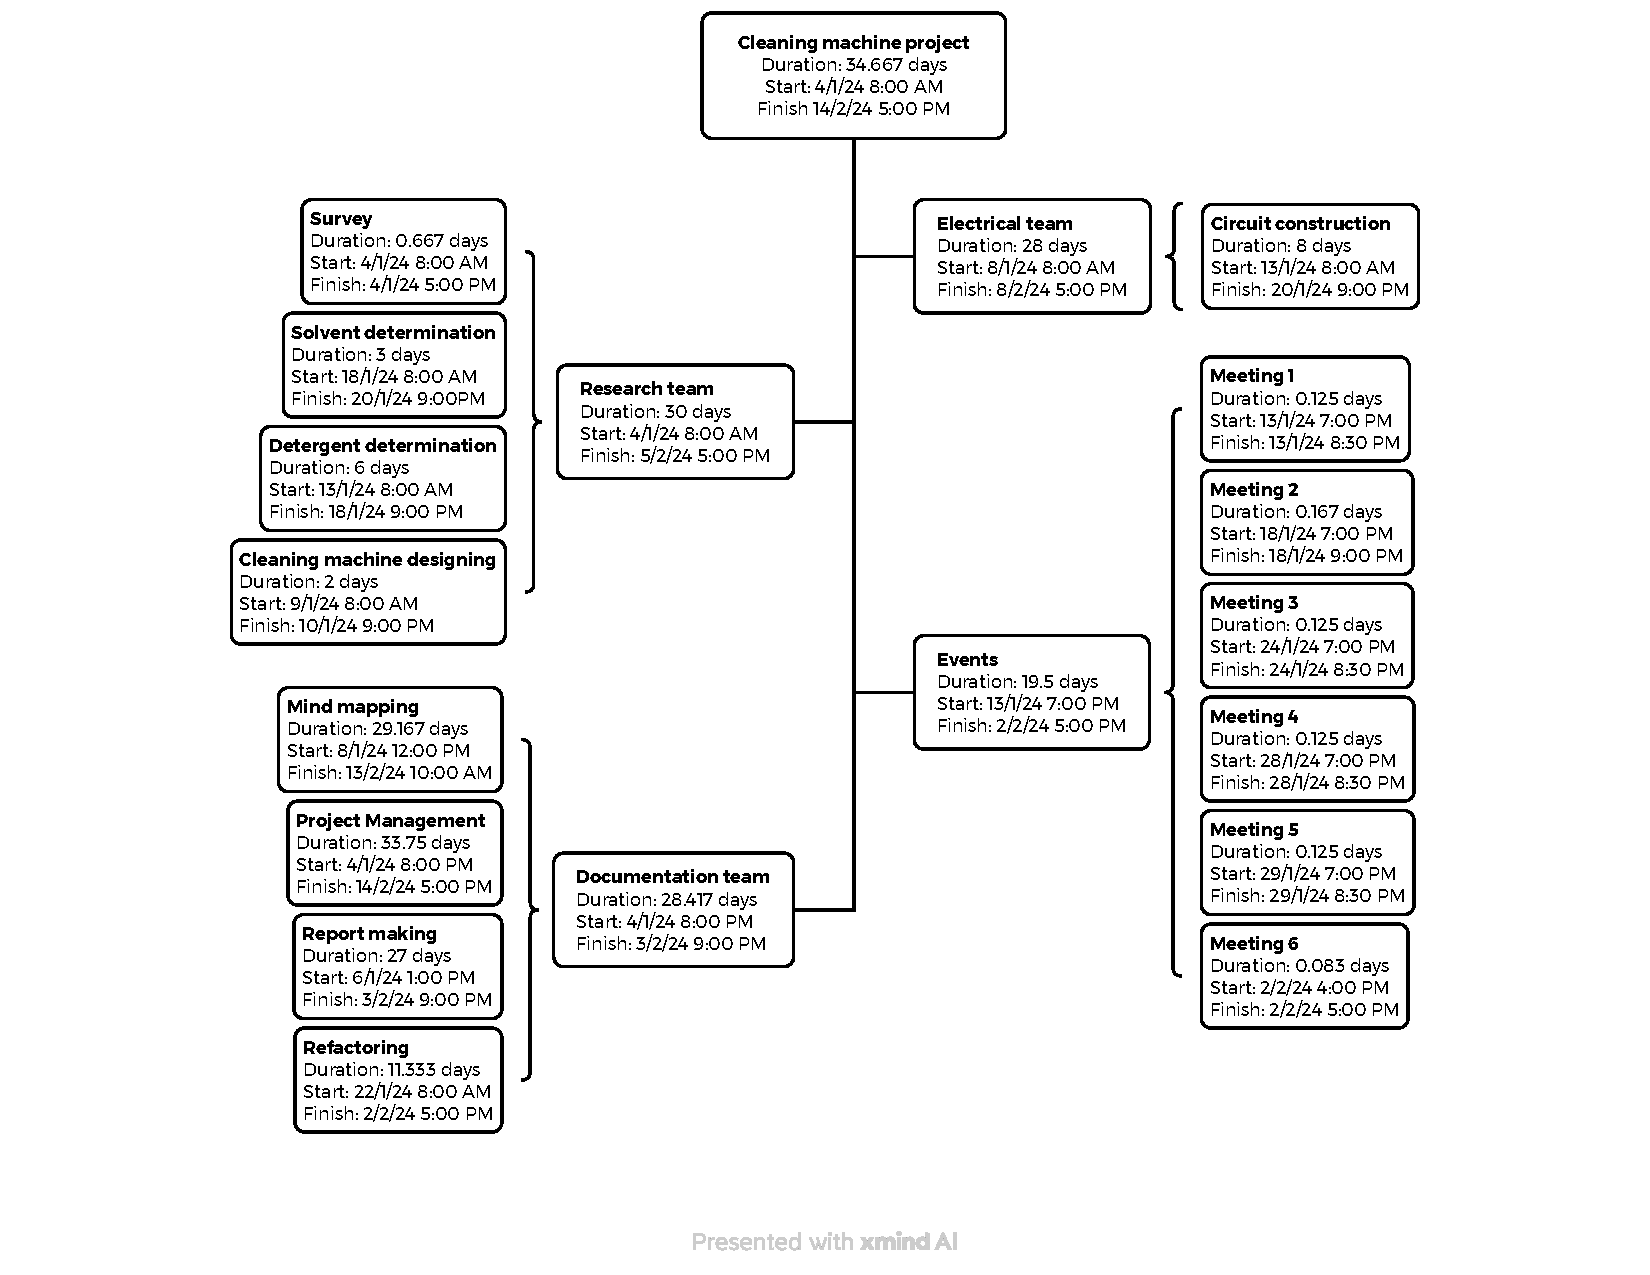
\includegraphics[width=0.97\textwidth]{Project/Network.png}
    \caption{Network Chart}
    \label{fig:enter-label}
\end{figure}
\newpage
\subsubsection*{\href{https://owncloud.iitd.ac.in/nextcloud/index.php/s/pnCtc4MAoRkQte2}{\textcolor{blue}{WBS}}}

\begin{figure}[h] \centering{
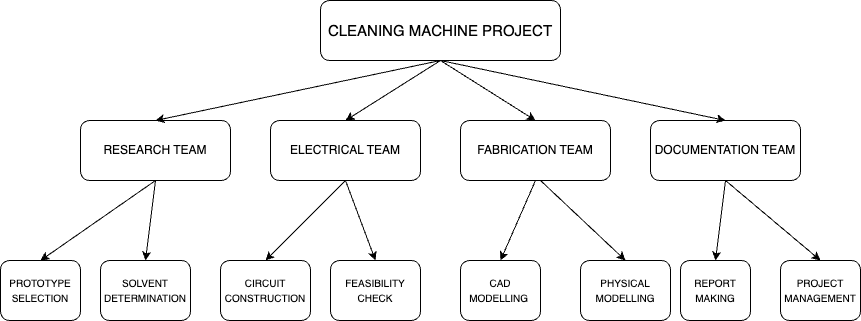
\includegraphics[scale=0.6,valign=c]{Project/wbs.png}
\caption{WBS}
\end{figure}
\newpage
\subsubsection*{\href{https://owncloud.iitd.ac.in/nextcloud/index.php/s/MDxAqgJGXYexDLy}{\textcolor{blue}{Gantt Chart}\index{\textcolor{blue}{Gantt Chart}}}}
\begin{figure}[htp] \centering{
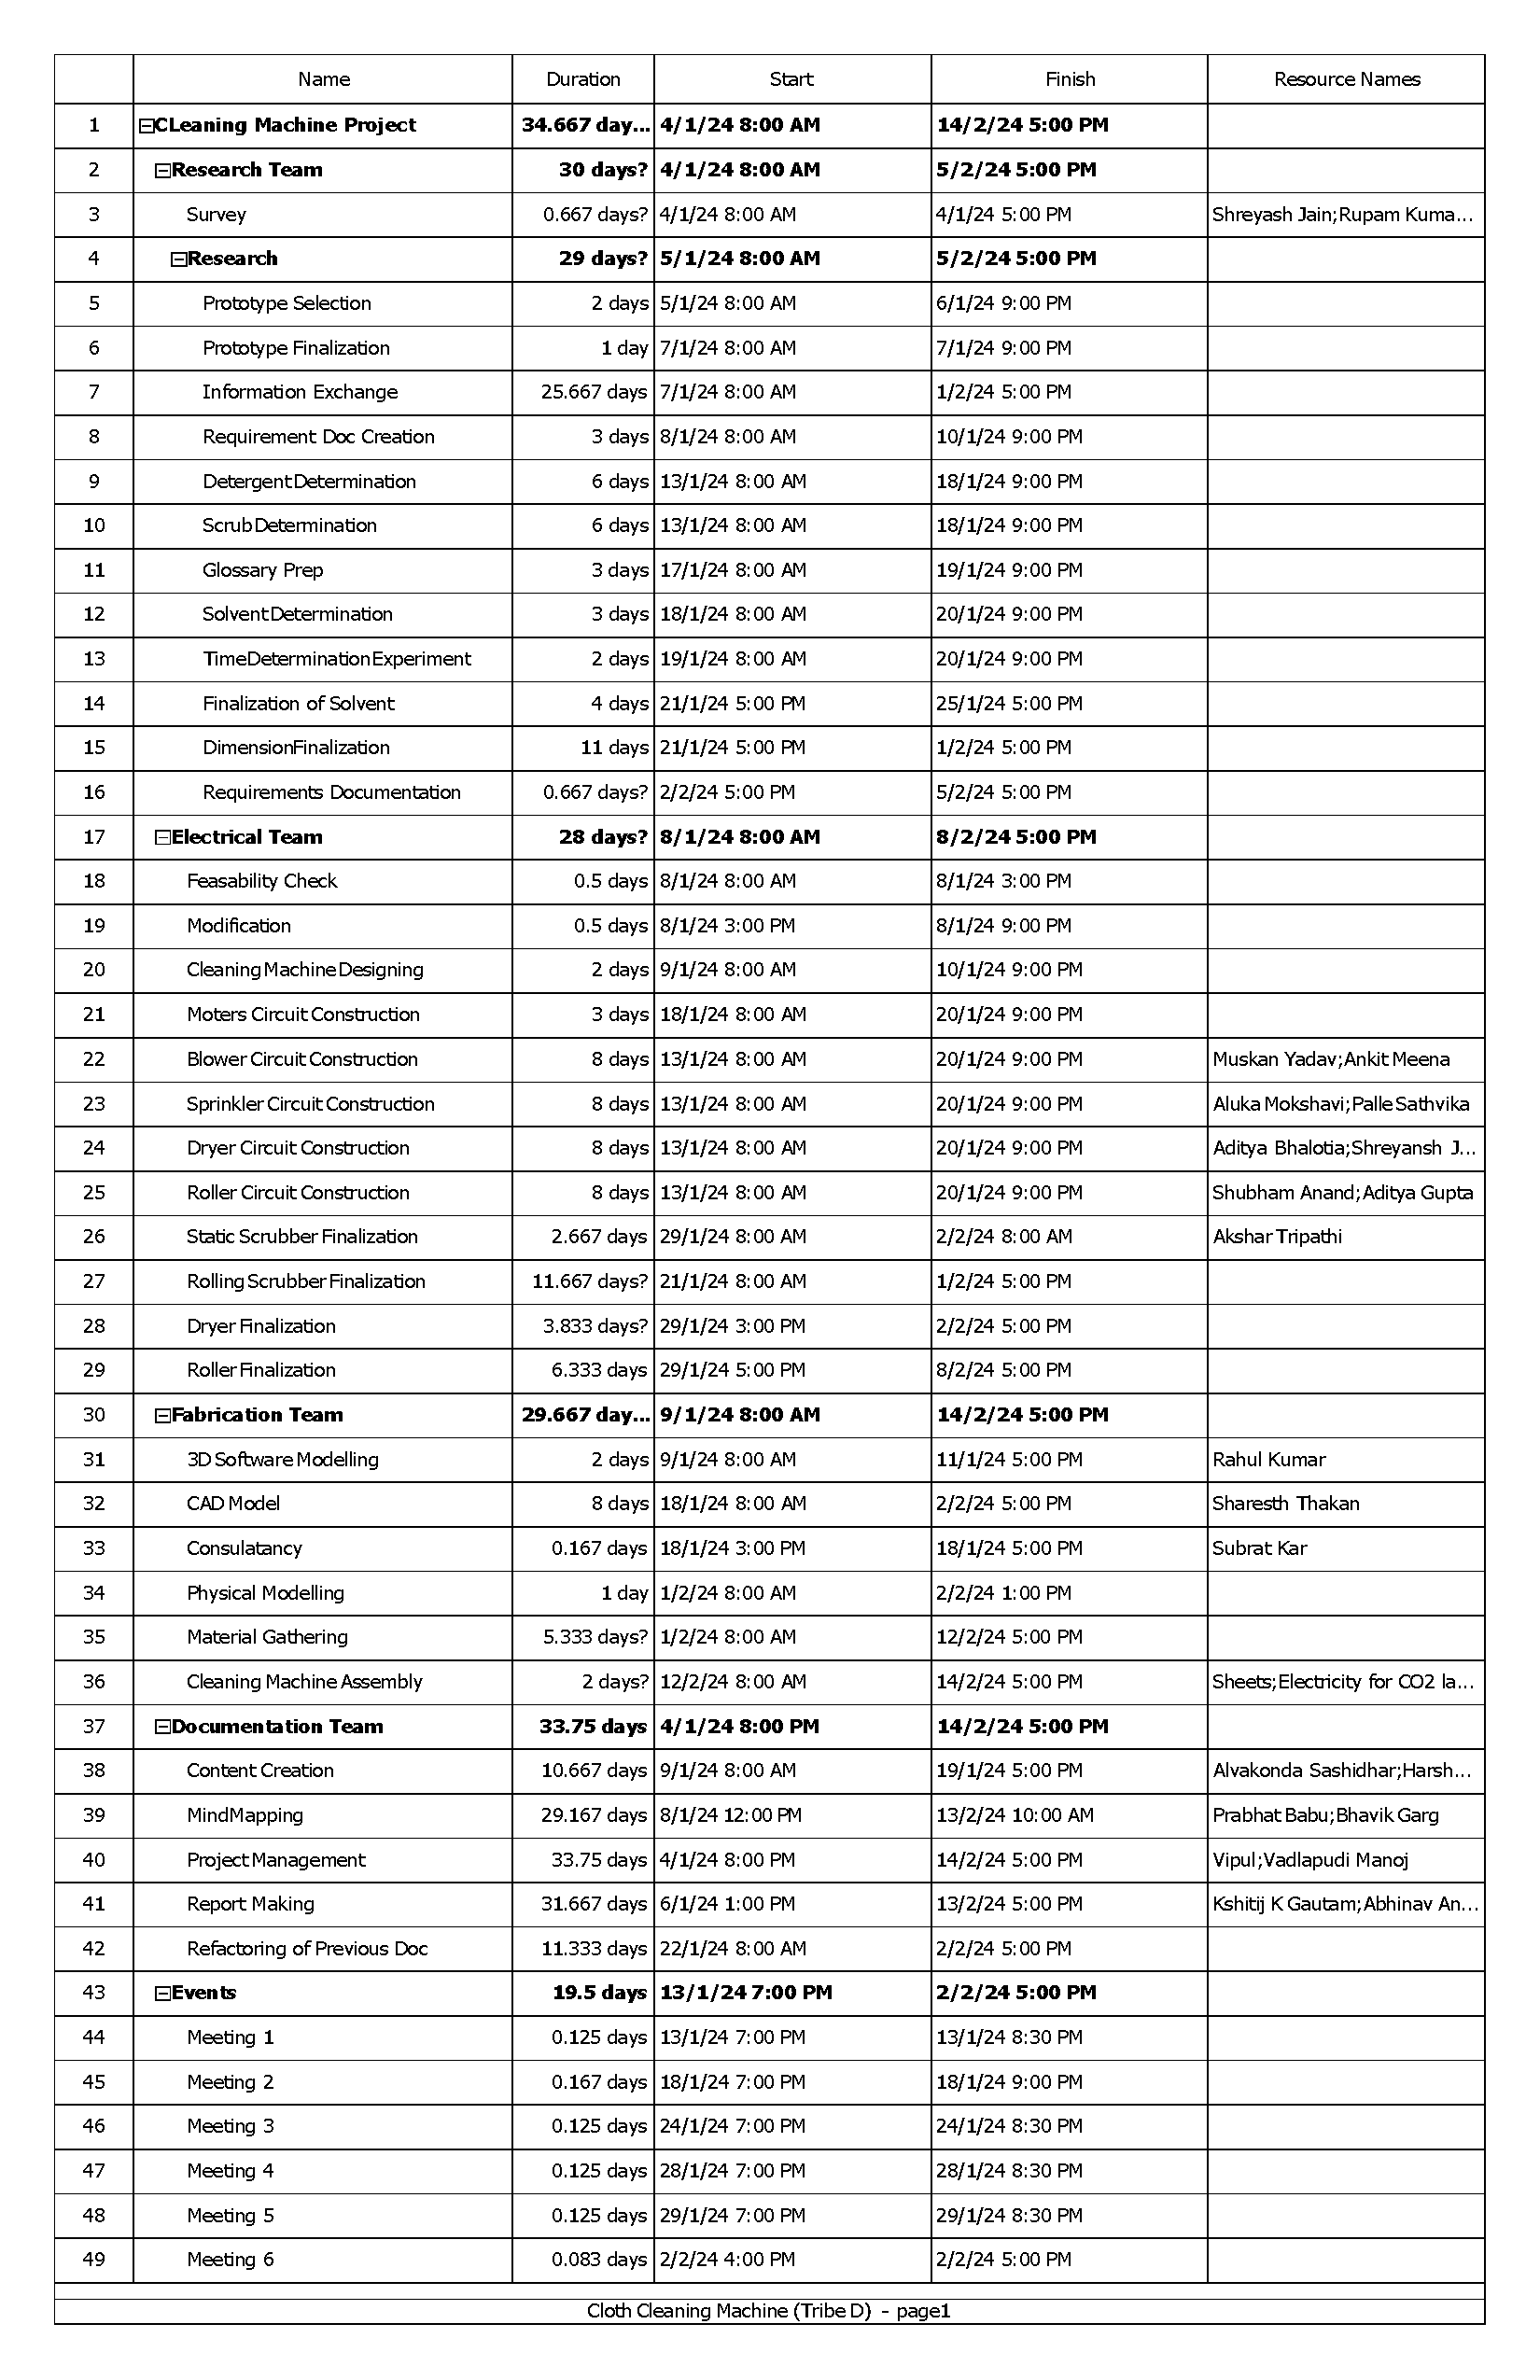
\includepdf[scale=0.85,pages={1}]{Project/gantt.pdf}
% \caption{Gantt Chart - 1}
\end{figure}

\newpage
Gantt Chart - 2
\begin{figure}[htp] \centering{
\includepdf[scale=0.89,pages={2}]{Project/gantt.pdf}
% \caption{Gantt Chart - 2}
\end{figure}
\newpage
\subsubsection*{\href{https://owncloud.iitd.ac.in/nextcloud/index.php/s/7HQLz7ibrgMm5mY}{\textcolor{blue}{Resource Breakdown}}}
\begin{figure}[htp] \centering{
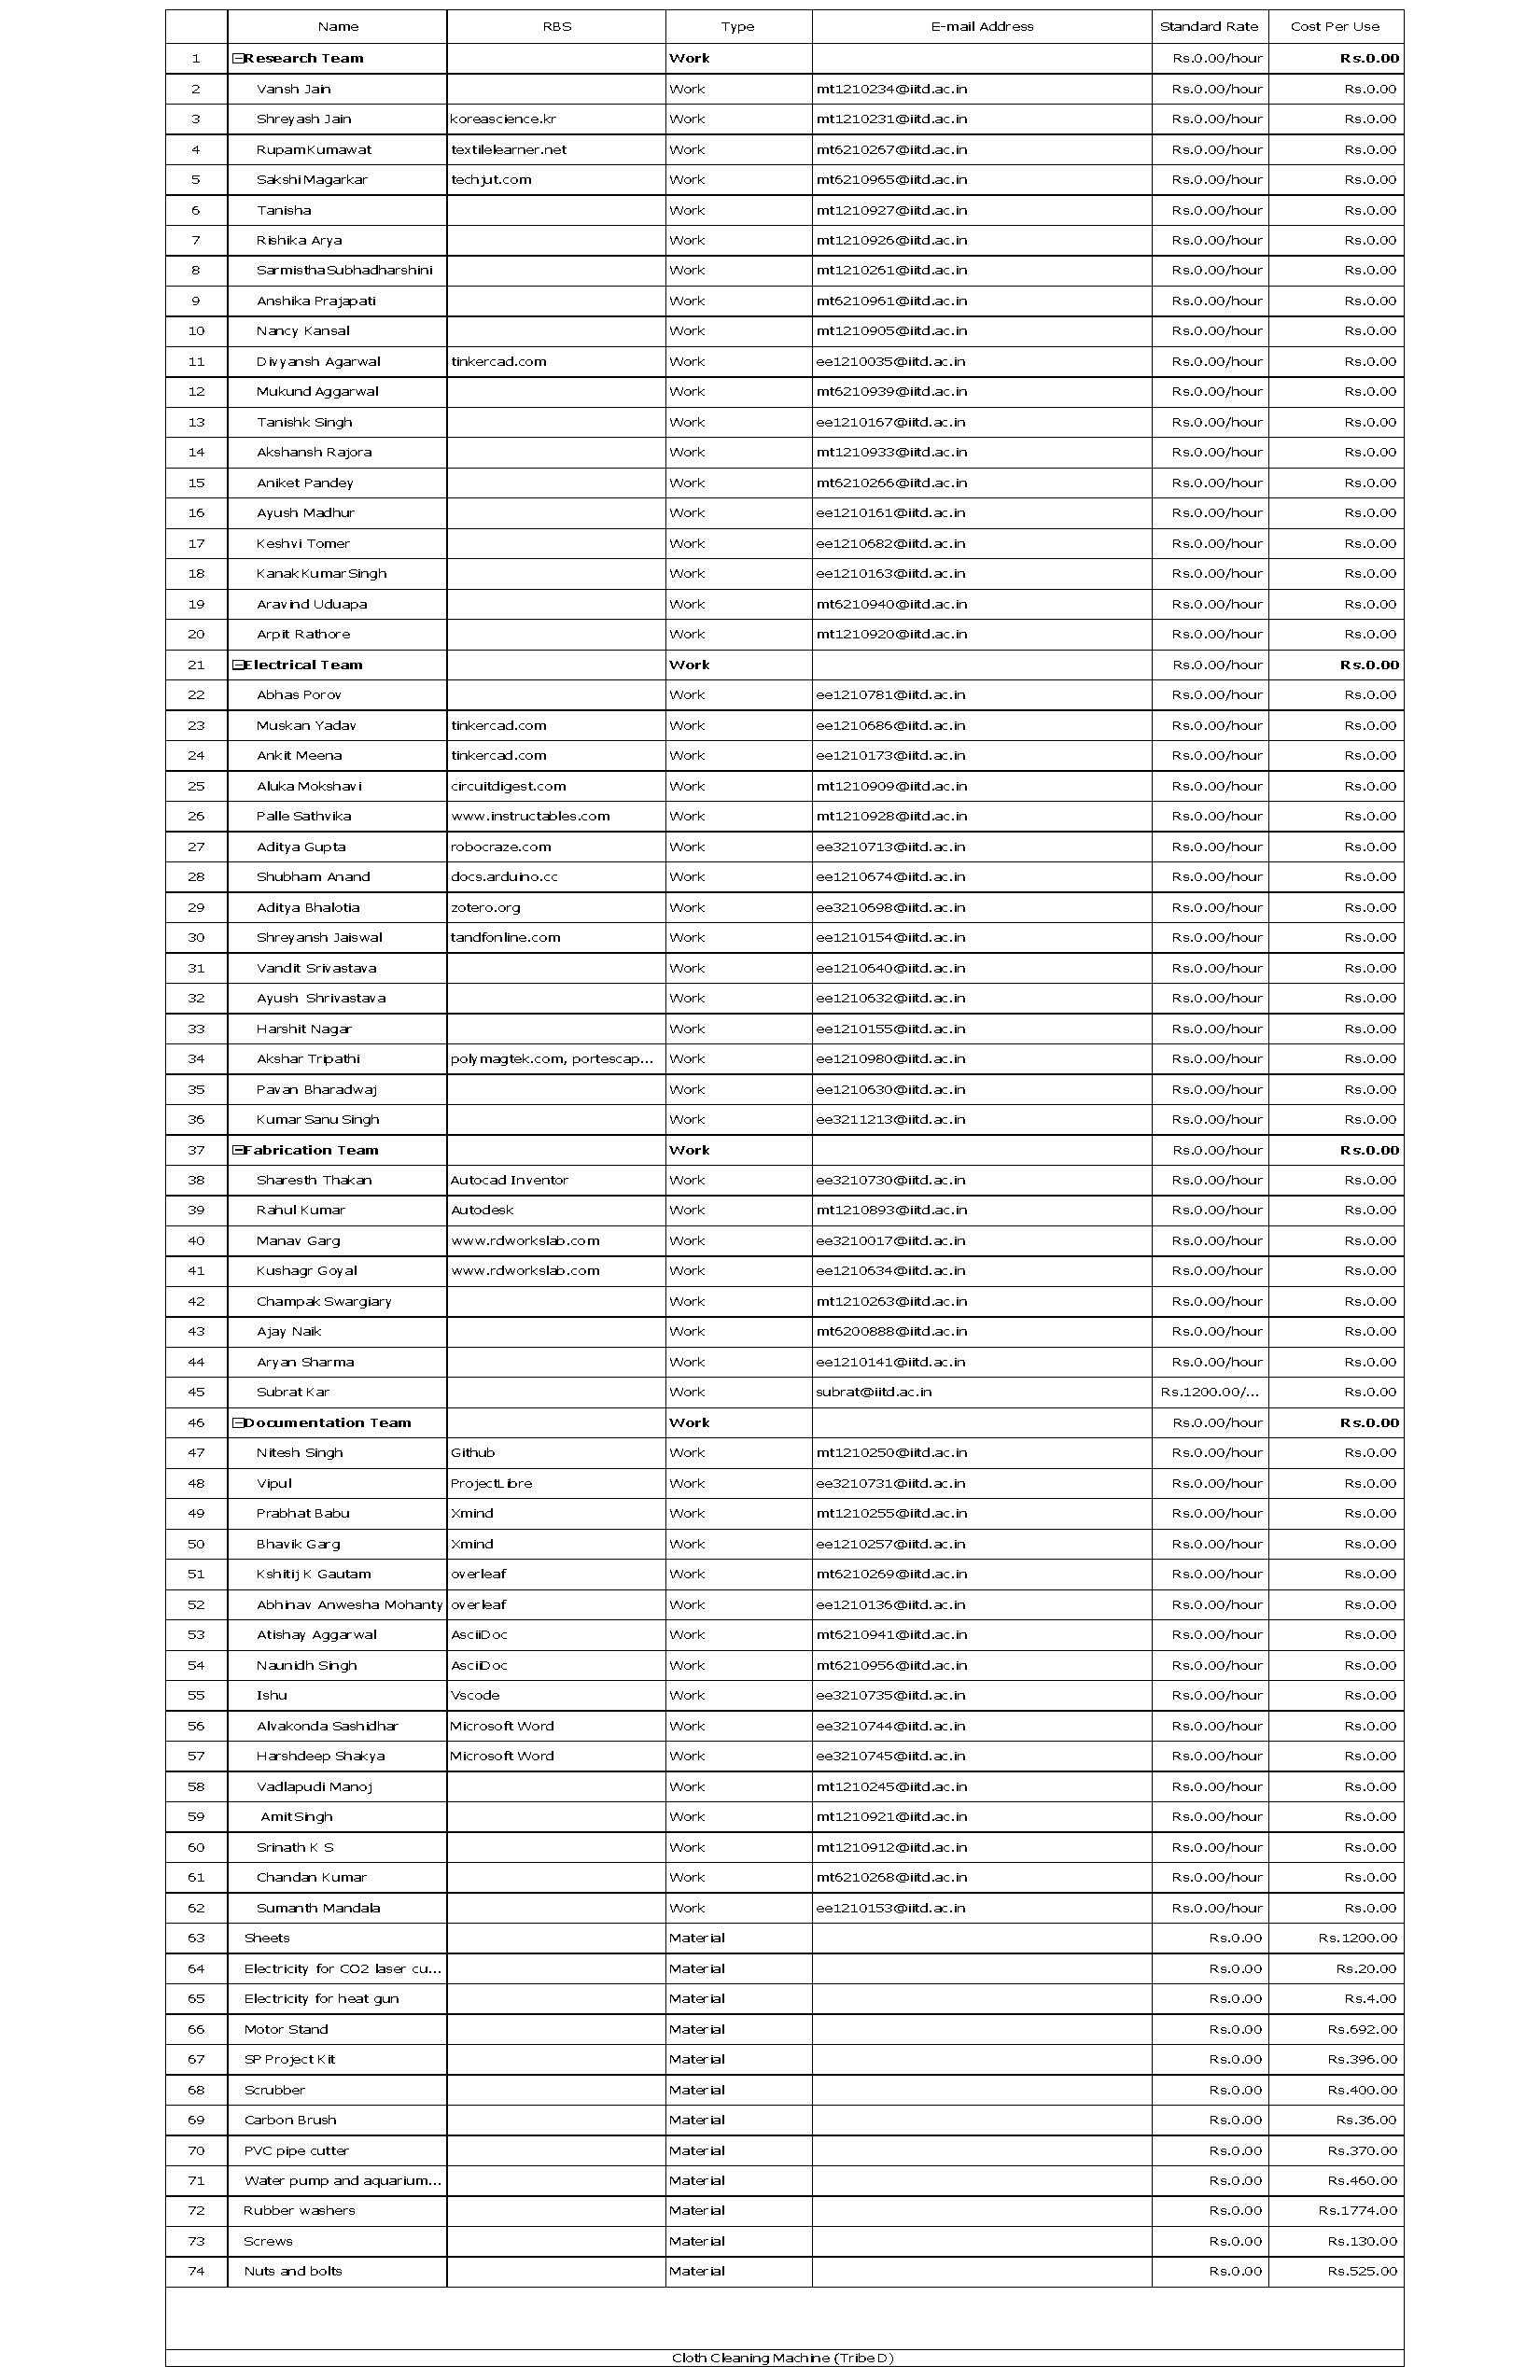
\includepdf[scale=0.78,pages=-]{Project/resource_breakdown.pdf}
% \caption{Resource Breakdown}
\end{figure}
% \begin{figure}[htp] \centering{
% \includepdf[scale=0.75,pages={2}]{Project/resource_breakdown.pdf}
% \caption{Resource Breakdown}
% \end{figure}
% \newpage
% \begin{figure}[h]
    
%     \begin{subfigure}{0.37\textwidth}
    
%         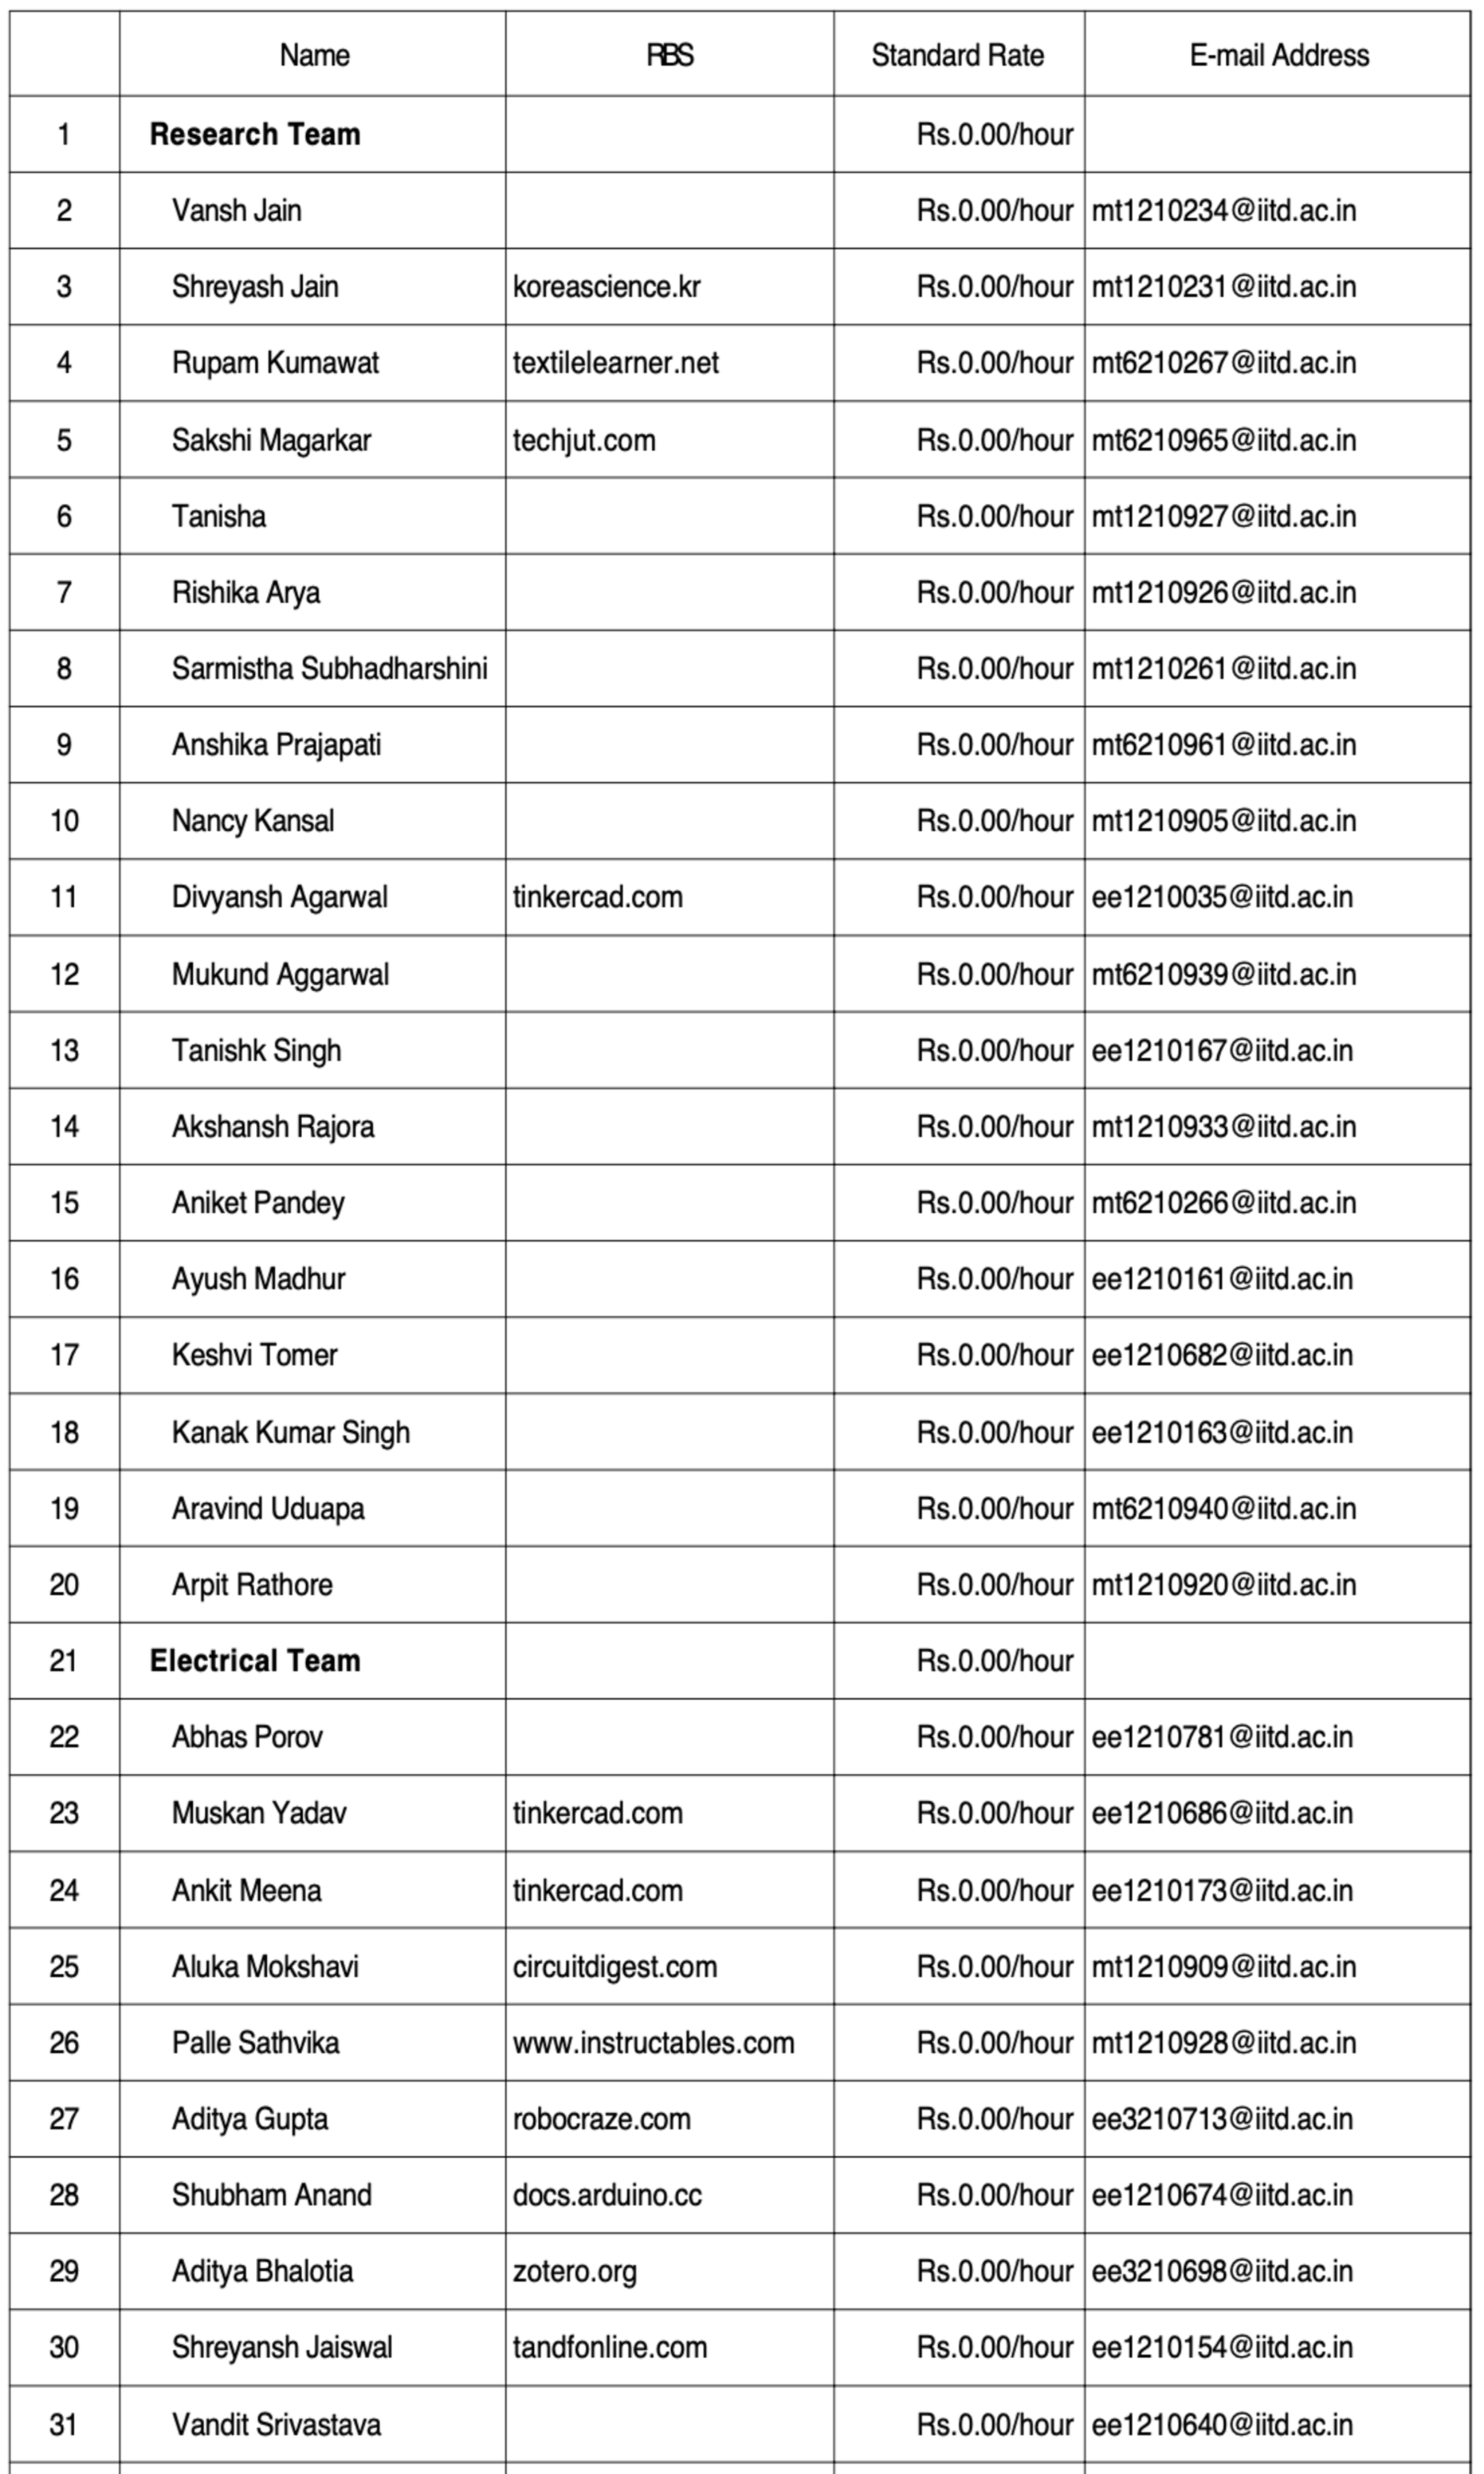
\includegraphics[width=\linewidth]{logos/resource_1.png}

%     \end{subfigure}\hspace{0.1\textwidth}%
%     \begin{subfigure}{0.37\textwidth}
        
%         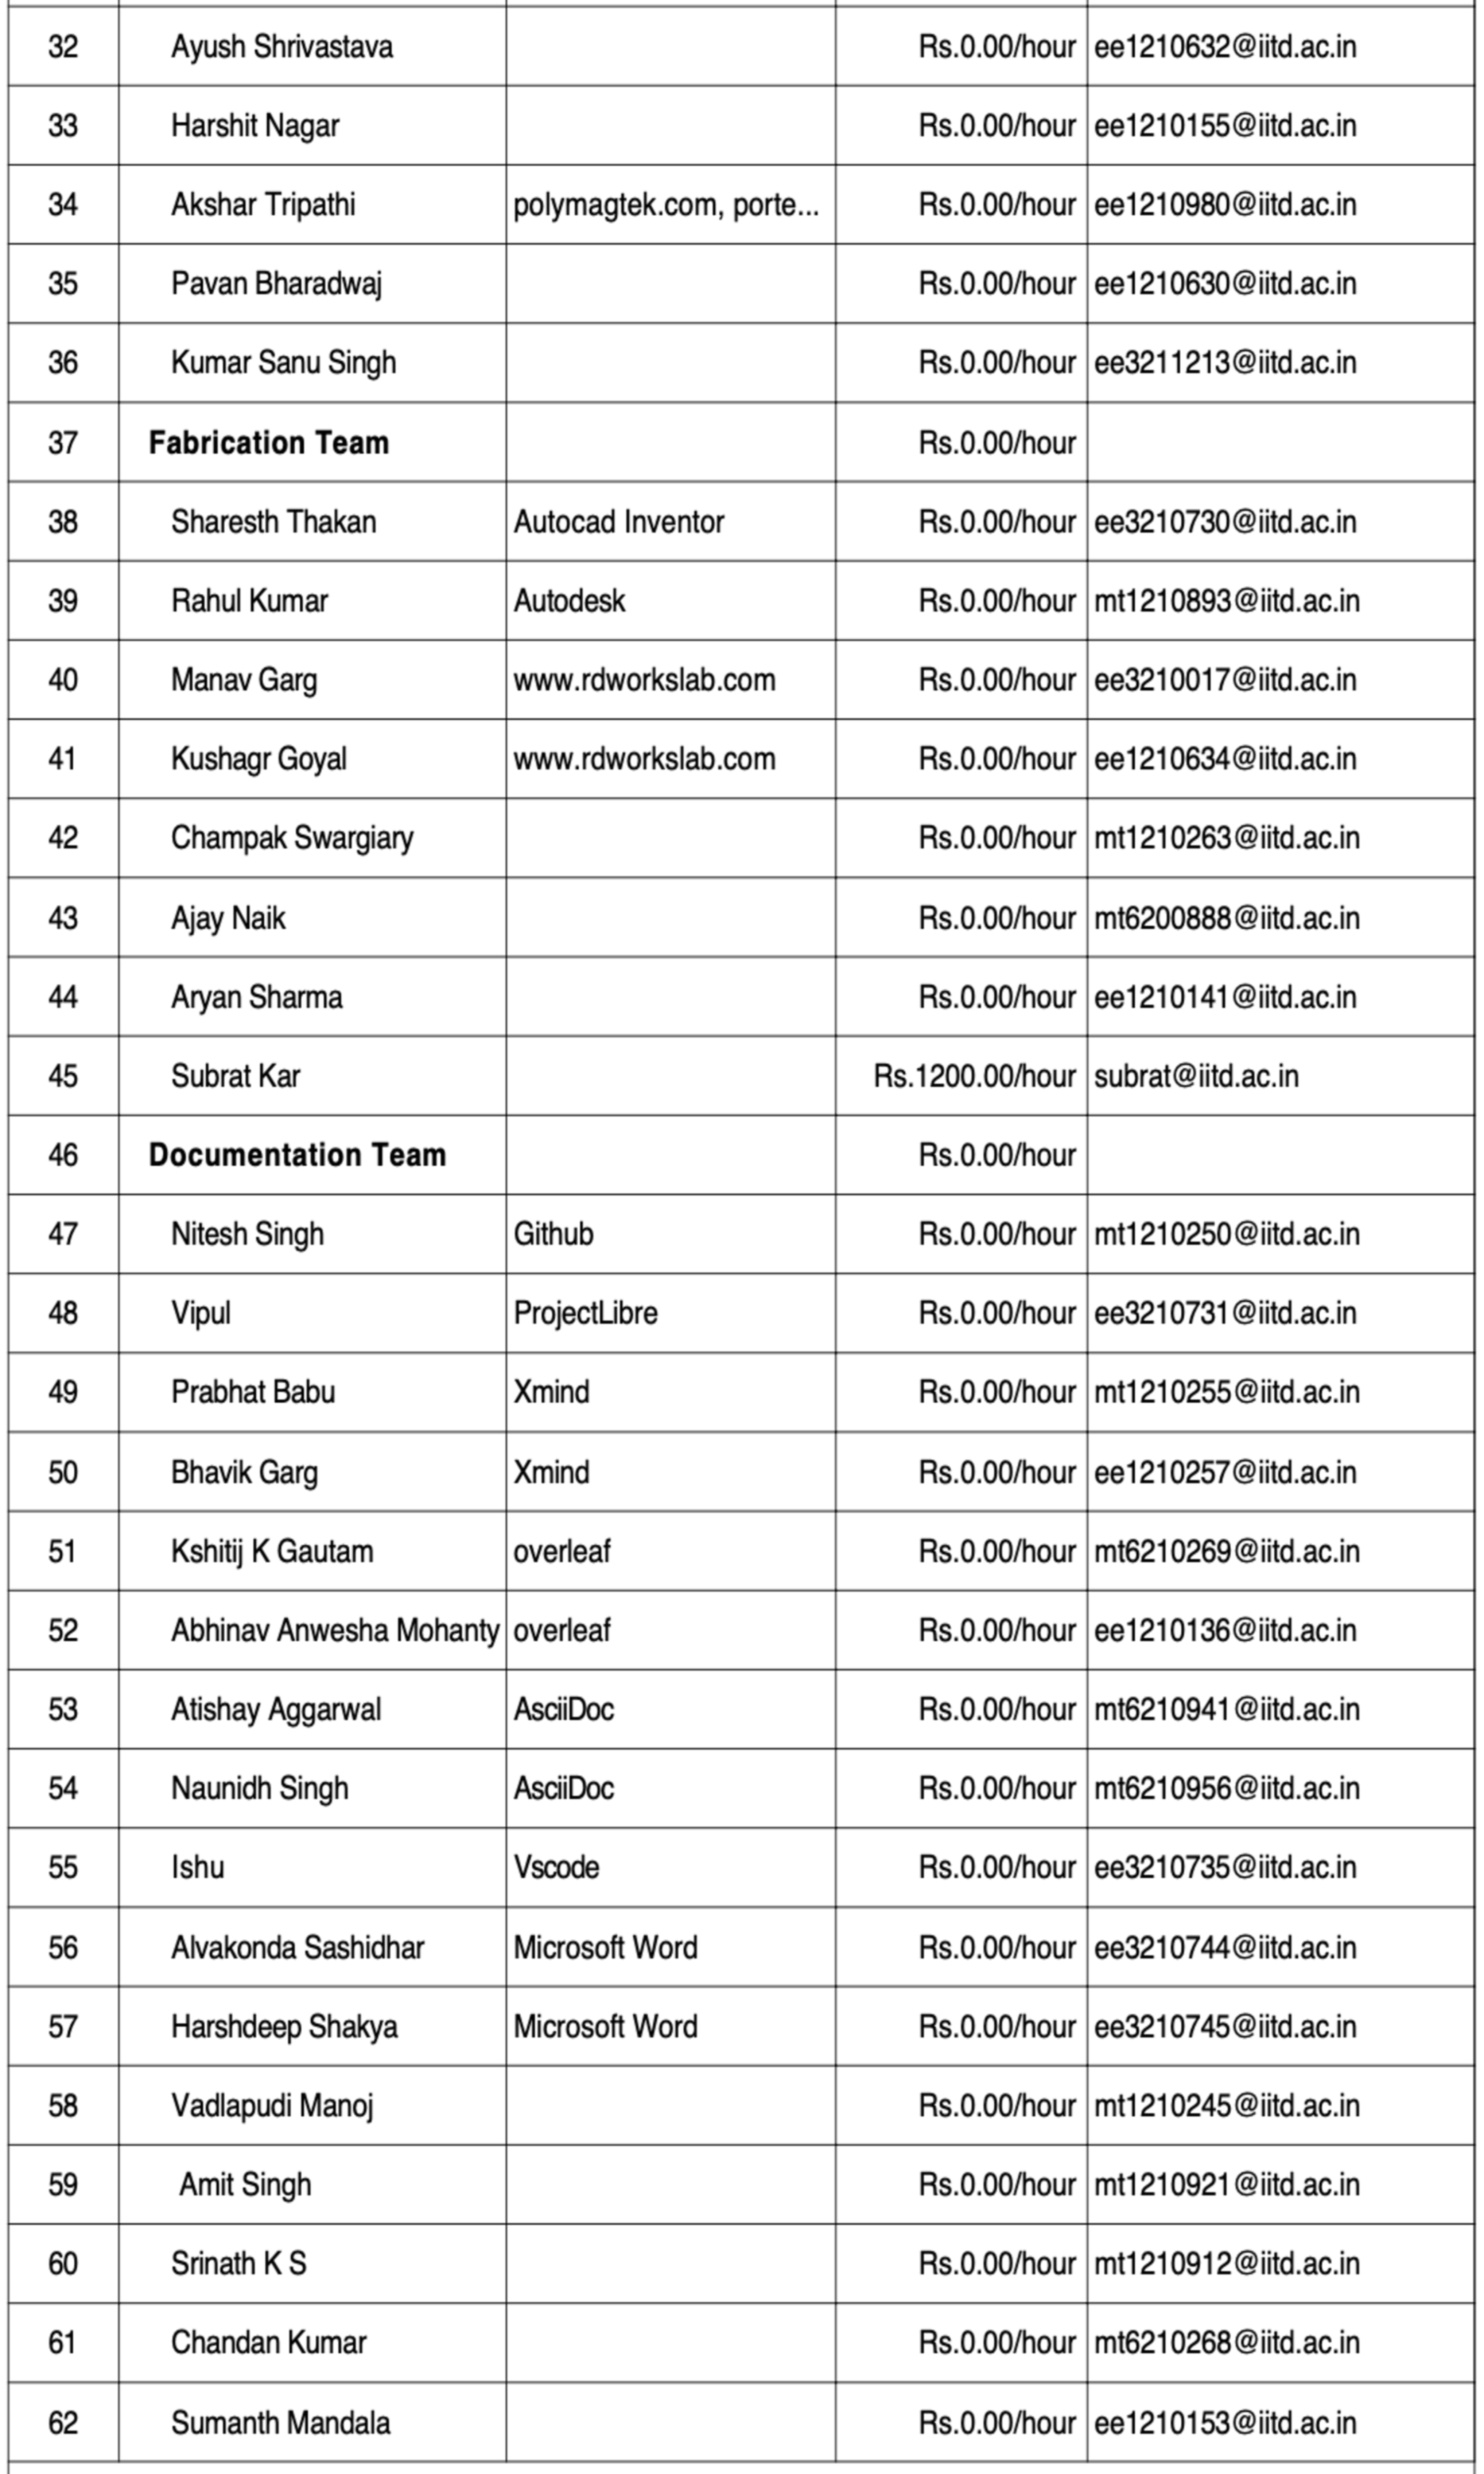
\includegraphics[width=\linewidth]{logos/resource_2.png}

%     \end{subfigure}
%     \caption{Resource Breakdown}
% \end{figure}


\newpage
\pagestyle{empty}
% \thispagestyle{fancy} % Apply the "fancy" page style only to this page
% \rhead{References}
\phantomsection
% \section*{References}\label{sec:references}
\addcontentsline{toc}{section}{References}
\renewcommand{\refname}{References}
\nocite{*}
\printbibliography
% \nocite{*}
   % \printbibliography
% \begin{itemize}
     % \cite{aqualogic_hot_2023} - \fullcite{aqualogic_hot_2023}
     % \cite{noauthor_4_nodate-1} - \fullcite{noauthor_4_nodate-1}\\
     % \cite{daniela_how_2017}-\fullcite{daniela_how_2017}
     % \cite{noauthor_54_nodate} - \fullcite{noauthor_54_nodate}
    %  \cite{aqualogic_hot_2023} - \fullcite{aqualogic_hot_2023}
    %  \cite{noauthor_arduino_nodate} - \fullcite{noauthor_arduino_nodate}
    %  \cite{noauthor_automatic_nodate} - \fullcite{noauthor_automatic_nodate}
    %  \cite{noauthor_buy_nodate-3} - \fullcite{noauthor_buy_nodate-3}
    %  \cite{noauthor_buy_nodate-2} - \fullcite{noauthor_buy_nodate-2}
    %  \cite{noauthor_buy_nodate-1} - \fullcite{noauthor_buy_nodate-1}
    %  \cite{chailoet_analytical_2018} - \fullcite{chailoet_analytical_2018}
    %  \cite{cleaners_dry_2020} - \fullcite{cleaners_dry_2020}
    %  \cite{noauthor_customized_nodate} - \fullcite{noauthor_customized_nodate}
    % % \item \cite{} - \fullcite{}
    %  \cite{gentlemans_gazette_how_2019} - \fullcite{gentlemans_gazette_how_2019}
    %  \cite{green_agitated_nodate} - \fullcite{green_agitated_nodate}
    % % \item \cite{kiron_classification_2014} - \fullcite{kiron_classification_2014}
    % % \item \cite{noauthor__nodate} - \fullcite{noauthor__nodate}
    % % \item \cite{noauthor_16_nodate} - \fullcite{noauthor_16_nodate}
    % % \item \cite{noauthor_buy_nodate} - \fullcite{noauthor_buy_nodate}
    % % \item \cite{noauthor_circuit_nodate-3} - \fullcite{noauthor_circuit_nodate-3}
    %  \cite{noauthor_does_nodate} - \fullcite{noauthor_does_nodate}
    %  \cite{noauthor_what_nodate} - \fullcite{noauthor_what_nodate}
    %  \cite{noauthor_how_2019} - \fullcite{noauthor_how_2019}
    %  \cite{noauthor_garment_nodate} - \fullcite{noauthor_garment_nodate}
    
% \end{itemize}
    
% \newpage
\pagestyle{plain}
\section*{}\phantomsection\label{sec:myindex}
\addcontentsline{toc}{section}{Index}
\printindex
\newpage
\newpage
\section*{}\phantomsection\label{sec: glossary}
\addcontentsline{toc}{section}{Glossary}
\thispagestyle{plain} 
\rhead{Glossary}
\renewcommand{\glossaryname}{Glossary}
\printglossaries\label{sec: glossary}

\newpage
\pagestyle{plain}

\section*{Appendix}\phantomsection\label{sec:appendix}
\addcontentsline{toc}{section}{Appendix}
\begin{table}[h]
      \centering
      \begin{tabular}{|l|r|}
        \hline
        \textbf{Word Count} & 9749 \\
        \hline
        \textbf{Number of Sentences} & 453 \\
        \hline
        \textbf{Number of Characters(Without Spaces)} & 51438 \\
        \hline
      \end{tabular}
      \caption{Document Statistics}
      \label{tab:documentstats}
    \end{table}
    \begin{table}[h]
      \centering
      \begin{tabular}{|l|r|}
        \hline
        \textbf{Readability (0-100)\footnote{This is a footnote.}} & 72.5 \\
        \hline
        \textbf{Gunning Fog Index (0-20)\footnote{This is a footnote.}} & 10.2 \\
        \hline
        \textbf{Flesch Reading Ease (0-100)\footnote{This is a footnote.}} & 53.7 \\
        \hline
        \textbf{Coleman Liau Index (0-17+)\footnote{This is a footnote.}} & 10.8 \\
        \hline
      \end{tabular}
      \caption{Readability Indices}
      \label{tab:readability}
    \end{table}
% \newpage
\rule{\linewidth}{0.5pt}
\textbf{}\newline
{\small 
\textbf{1. Readibility}\newline
\textit{Score Range: 0-100}\newline
Explanation: The Readability (0-100) score, measures how easy or difficult a piece of text is to read. The higher the score, the easier the text is to understand. The score is calculated based on the average sentence length and the average number of syllables per word in the text.
\textbf{}\newline
\textbf{2. Gunning Fog Readability}\newline
\textit{Score Range: 0-20}\newline
Explanation: The Gunning Fog Index estimates the years of formal education needed to understand a piece of text. The higher the index, the more difficult the text is to comprehend. It considers the average sentence length and the percentage of complex words (words with three or more syllables).
\textbf{}\newline
\textbf{3. Flesch Reading Ease}\newline
\textit{Score Range: 0-100}\newline
Explanation: The Flesch Reading Ease score is a measure of how easy or difficult a piece of text is to read. The higher the score, the easier the text is to understand. The formula takes into account the average sentence length and the average number of syllables per word.
\textbf{}\newline
\textbf{4. Coleman Liau Readability Index}\newline
\textit{Score Range: 0-17+}\newline
Explanation: The Coleman Liau Index determines the readability of a text by using characters per word and words per sentence. It provides an estimate of the U.S. school grade level required to comprehend the text. Higher scores indicate more difficult readability.

}


\end{document}  